%%%%%%%%%%%%%%%%%%%%%%%%%%%%%%%%%%%%%%%%%%%%%%%%%%%%%%%%%%%%%%%%%%%%%%%%%%%%%%%
%% LaTeX-Vorlage für Abschlussarbeiten                                       %%
%% (TH Köln -Campus Gummersbach, Fak. 10)                                    %%
%%                                                                           %%
%% Gemäß dem Merkblatt zur Anfertigung von Projekt-, Bachelor-, Master- und  %%
%% Diplomarbeiten der Fakultät 10 von Frau Prof. Dr. Halfmann &              %%
%% Herr Prof. Dr. Rühmann (Version vom 27.01.2008)                           %%
%%                                                                           %%                                                                            
%% Bitte sprechen Sie unbedingt mit Ihrer Betreuerin bzw. Ihrem Betreuer     %%
%% bezüglich der Ausgestaltung Ihrer Arbeit!                                 %%
%%                                                                           %%
%%                                                                           %%
%% MERKKASTEN IN DIESER VORLAGE:                                             %%
%% In dieser Vorlage finden Sie Merkkasten, die Ihnen Informationen          %%
%% zu bestimmten, formalen Aspekten geben. Sprechen Sie immer auch mit       %% 
%% Ihrer Betreuerin bzw. Ihrem Betreuer dazu an.                             %%                       
%% Für die eigene Verwendung der Vorlage entfernen oder kommentieren Sie die %%
%% Merkkasten. Die betreffenden Bereiche für die Merkkasten in der Vorlage   %%
%% sind wie folgt kommentiert: <MERKKASTEN> ... </MERKKASTEN>.               %%                            %%                                                                           %%
%%                                                                           %%
%% LIZENZ:                                                                   %%
%% Diese Vorlage darf nicht kommerziell verbreitet                           %%
%% werden. Eine nicht-kommerzielle Weitergabe ist                            %% 
%% gestattet.                                                                %%
%%                                                                           %%
%% Von Ludger Schönfeld, M. Sc.,                                             %%
%% 2014-2017                                                                 %%
%%%%%%%%%%%%%%%%%%%%%%%%%%%%%%%%%%%%%%%%%%%%%%%%%%%%%%%%%%%%%%%%%%%%%%%%%%%%%%%

%%%%%%%%%%%%%%%%%%%%%%%%%%%%%%%%%%%%%%%%%%%%%
%% HEADER                                  %%
%%%%%%%%%%%%%%%%%%%%%%%%%%%%%%%%%%%%%%%%%%%%%
\documentclass[a4paper,12pt,oneside]{article}
% Optionen:
% - a4paper => DIN A4-Format
% - 12pt    => Schriftgröße (weitere  
%              grundlegende Fontgrößen: 10pt, 11pt)
% - oneside => Einseitiger Druck

%% Verwendete Pakete:
\usepackage[ngerman]{babel} % für die deutsche Sprache
\usepackage{caption} % Für schönere Bildunterschriften
\usepackage[T1]{fontenc} % Schriftkodierung (Für Sonderzeichen u.a.)
\usepackage[utf8]{inputenc} % Für die direkte Eingabe von Umlauten im Editor u.a.
\usepackage{fancyhdr} % Für Kopf- und Fußzeilen
\usepackage{lscape} % Für Querformat

%% Schriften (Beispiele)
%% Weitere LaTeX-Schriften im "LaTeX Font Catalogue"
%% unter: http://www.tug.dk/FontCatalogue/.
%% ACHTUNG: Ggf. müssen Schriften noch installiert 
%% werden!

% Serifen-Schriften:
\usepackage{lmodern} % Schriftart "Latin Modern"
%\usepackage{garamond} % Schriftart "Garamond"

%Sans Serif-Schriften:
%\usepackage[scaled]{uarial}
%\usepackage[scaled]{helvet}
%%--------------
\usepackage[normalem]{ulem} % Für das Unterstreichen von Text z.B. mit \uline{}
\usepackage[left=3cm,right=2cm,top=1.5cm,bottom=1cm,
textheight=245mm,textwidth=160mm,includeheadfoot,headsep=1cm,
footskip=1cm,headheight=14.599pt]{geometry} % Einrichtung der Seite 

\usepackage{graphicx} % Zum Laden von Graphiken
% INFO: Graphiken einbinden
%
% \includegraphics[scale=1.00]{dateiname}
%
% => Ausgabeformat: PDF-Dokument:
%    Es können die folgenden (Graphik-)formate eingebunden
%    werden: .jpg, .png, .pdf, .mps
% 
% => Ausgabeformat: DVI/PS:
%    Folgende (Graphik-)formate werden unterstützt:
%    .eps, .ps, .bmp, .pict, .pntg
\usepackage{epstopdf}

% Pakete für Tabellen
\usepackage{tabularx} % Einfache Tabellen
\usepackage{longtable} % Tabellen als Gleitobjekte (für die Aufteilung bei langen 
 %Tabellen über mehrere Seiten)
\usepackage{multirow} % Für das Verbinden von Zeilen innerhalb einer Tabelle mit
 % \multirow{anzahl}{*}{Text}

% (Zusatz-)Pakete für Formeln
\usepackage{amsmath}
\usepackage{amsthm}
\usepackage{amsfonts}

\usepackage{setspace} % Paket zum Setzen des Zeilenabstandes
% INFO: Zeilenabstand setzen:
%
% Befehle:
% - \singlespacing  => 1-zeilig (Standard)
% - \onehalfspacing => 1,5-zeilig
% - \doublespacing  => 2-zeilig 
\onehalfspacing % Zeilenabstand auf 1,5-zeilig setzen

% Emotes in LaTeX

% Farbboxen (für die Merkkästen in dieser Vorlage):
\usepackage{tcolorbox}
\tcbset{colback=white,colframe=orange,
        fonttitle=\bfseries}

\usepackage[colorlinks,pdfpagelabels,pdfstartview=FitH,
bookmarksopen=true,bookmarksnumbered=true,linkcolor=black,
plainpages=false,hypertexnames=false,citecolor=black]{hyperref} % Für Verlinkungen
% INFO: Verlinkungen mit dem hyperref-Paket:
%
% Die Angabe von URLs mit dem Befehl \url{} erlaubt einen
% gesonderten Umgang mit Weblinks. Denn die Links werden verlinkt.
% Auch erfolgt automatisch am Zeilenende ein Umbruch des Links.
% Es ist auch nicht erforderlich, Sonderzeichen in der URL manuell zu 
% entschärfen.
%
% TIPP: Sollte ein Umbuch bei einem Link nicht automatisch erfolgen, so kann
% das daran liegen, dass ein/mehrere Zeichen zusätzlich angegeben werden müssen,
% an dem der Link umbrochen werden kann.
% Dies kann mit folgendem Befehl erfolgen (Beispiel):
% \renewcommand*\UrlBreaks{\do-\do_}

% Das Paket "biblatex" für autom. 
% Literaturverzeichnisse:
\usepackage{csquotes} % Für sprachangepasste Anführungszeichen
\usepackage[backend=biber,style=authoryear,citestyle=apa]{biblatex}
\addbibresource{bib/literatur.bib}

\title{Entwicklung von Darstellungs- und Interaktionsmöglichkeiten in Virtual Reality für das Cranach Digital Archive}
\author{Nikolas Beckel (11103435)}
\date{15. September 2020}
% Use \maketitle for generated title

%%%%%%%%%%%%%%%%%%%%%%%%%%%%%%%%%%%%%%%%%%%%%
%% DOKUMENT                                %%
%%%%%%%%%%%%%%%%%%%%%%%%%%%%%%%%%%%%%%%%%%%%%
\begin{document}
  % Unbeschriftetes Vorblatt (Leere Seite)
  \pagestyle{empty} % Seite ohne Kopf- und Fußzeilen
  \newpage % Neue Seite
  \section*{}  
           % Ausgelagerte LaTeX-Datei (hier: leereSeite.tex) einbinden

  \newpage

  % Deckblatt
  \pagestyle{empty}
  \begin{titlepage}
    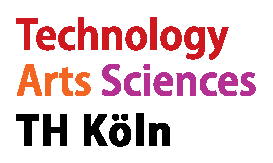
\includegraphics[scale=1.00]{img/logo_TH-Koeln_CMYK_22pt}\\
    \begin{center}
      \Large
      Technische Hochschule Köln\\
      Fakultät für Informatik und Ingenieurwissenschaften\\
      \hrule\par\rule{0pt}{2cm} % Horizontale Trennlinie  mit 2 cm Abtand nach unten erzeugen
      \LARGE
      \textsc{B A C H E L O R A R B E I T}\\
      \vspace{1cm} % Vertikaler Abstand von 1cm erzeugen
      \huge
      Entwicklung von Darstellungs- und Interaktionsmöglichkeiten in Virtual Reality für das Cranach Digital Archive\\
      \vspace{1cm}
      \large
      Vorgelegt an der TH Köln\\
      Campus Gummersbach\\
      im Studiengang\\
      Medieninformatik\\ 
      \vspace{1.0cm}
      ausgearbeitet von:\\
      \textsc{Nikolas Beckel}\\
      (Matrikelnummer: 11103435)\\
      \vspace{1.5cm}
      \begin{tabular}{ll} % Einfache Tabelle ohne Rahmen, mit 2 Spalten erzeugen
          \textbf{Erster Prüfer:} & Prof. Christian Noss \\
          \textbf{Zweiter Prüfer:} & Matthias Groß \\
      \end{tabular}
      \vspace{1.5cm}
      \\Gummersbach, im November 2020
    \end{center}    
  \end{titlepage}

  % Inhaltsverzeichnis
  \tableofcontents
  \newpage

  % Abbildungsverzeichnis
  \section*{Abbildungsverzeichnis}
  \addcontentsline{toc}{section}{Abbildungsverzeichnis} % Manuellen Eintrag im Inhaltsverzeichnis erzeugen
  \renewcommand{\listfigurename}{} % Name des Abbildungsverzeichnisses ändern
  \listoffigures

  % Tabellenverzeichnis
  \section*{Tabellenverzeichnis}
  \addcontentsline{toc}{section}{Tabellenverzeichnis} % Manuellen Eintrag im Inhaltsverzeichnis erzeugen
  \renewcommand{\listtablename}{} % Name des Abbildungsverzeichnisses ändern
  \listoftables
  \newpage

  \pagestyle{plain}

  % Die Bachelorarbeit
  \section{Einleitung}
    Virtual Reality ist nicht mehr nur Zukunftsmusik oder ein Anwendungsbereich für Forscher\footnote{Grundlegend ist in diesem Zusammenhang anzumerken, dass im Rahmen dieser Bachelorarbeit nicht alle Gender berücksichtigt werden und somit das geschlechtliche Neutrum verwendet wird.}
    großer Konzerne. Immer mehr kommt Virtual Reality auf den Massenmarkt, beispielsweise
    in der Spiele- oder Automobilindustrie. Wo zu Beginn
    leistungsfähige Computer benötigt wurden, entstehen heutzutage All-in-One VR-Brillen\footnote{Oculus Quest 2 - All-in-One VR-Brille | \url{https://www.oculus.com/quest-2/} (22.11.2020).}.
    Die Anwendungsbereiche von Virtual Reality sind vielfältig: Gaming, Unterhaltung durch VR-Filme oder
    das Treffen von Freunden in virtuellen Welten\footnote{Mozilla Hubs | \url{https://labs.mozilla.org/projects/hubs/} (22.11.2020).}.
    Die Pandemie durch das Virus SARS-CoV-2 hat uns gezeigt, dass immer mehr digitale Lösungen
    benötigt werden. Die Schulen zeigten, dass im Bereich digitaler Unterricht
    noch großte Defizite aufzuweisen sind. Aber auch Unternehmen hatten mit der Umstellung
    auf Home Office und digitale Meetings Startschwierigkeiten.
    Durch solche Pandemien bekommen 
    plötzlich Anwendungsbereiche, die nicht als
    notwendig betrachtet wurden, völlig neue Relevanz.
    Mit Virtual Reality ist der Benutzer 
    an keinen Ort gebunden und kann Meetings oder Unterricht
    statt in der realen Welt, in einer virtuellen Welt ausführen. Von der realen Welt
    losgelöst, entstehen so auch völlig neue Möglichkeiten, diese auszuführen. Unterricht kann
    durch multimedialen Einsatz interaktiver wie auch innovativer gestaltet werden, ebenso
    Meetings im Unternehmensbereich. \\
    Aber auch für Museen entstehen durch Virtual Reality neue Möglichkeiten und Chancen,
    da das Loslösen von der realen Welt neue Perspektiven erlaubt. Der Besucher eines
    Museums muss nicht mehr nur vor dem Ausstellungsstück stehen und dieses betrachten,
    sondern kann beispielsweise die Entstehung dieses Ausstellungsstücks in einer
    nachgestellten virtuellen Realität erleben und dabei die Emotionen des Künstlers
    direkt miterleben. Oder das Darstellen von großen Datenmengen, worüber auch das
    Cranach Digital Archive verfügt, kann in einer dreidimensionalen Umgebung beispielsweise
    ähnlich wie ein neuronales Netz dargestellt werden, um Beziehungen zwischen einzelnen
    Gemälden darzustellen. \\
    Das Potenzial ist theoretisch unendlich, da eine virtuelle Realität, ohne die Regeln
    unserer Physik, viele Möglichkeiten der Darstellung bietet.
    Doch unzählige Chancen können ebenso einige Risiken aufweisen. \\
    Das Ziel dieser Bachelorarbeit ist herauszufinden, 
    welche Möglichkeiten bestehen, um
    Gemälde und Dokumente von Lucas Cranach in einer virtuellen Welt darzustellen. 
    Darüber hinaus soll geprüft werden, wie Benutzer mit diesen Darstellungsmöglichkeiten 
    interagieren können. Dabei sollen die Chancen und Risiken für Museen
    berücksichtigt und miteinbezogen werden. \\  
    Dafür wird das Cranach Digital Archive\footnote{Cranach Digital Archive | \url{http://lucascranach.org/} (22.11.2020).}
    als Ressource genutzt. Lucas Cranach der Ältere war einer der bedeutendsten
    deutschen Künstler der Renaissance und hatte eine gute und freundschaftliche
    Beziehung zu Martin Luther. Dabei sollen aktuelle Entwicklungen und Technologien, 
    unter anderem aus dem musealen Bereich, 
    miteinbezogen und deren Erkenntnisse der Entwicklung berücksichtigt werden.
    Auf Basis dieser Ergebnisse wurden mehrere Prototypen entwickelt,
    die zeigen, wie Virtual Reality im Bereich Kunst und Kultur angewendet werden kann. \\
  \section{Grundlage und Datenbasis}
    In diesem Kapitel wird auf die Grundlagen von Virtual Reality, auf den Künstler Lucas Cranach 
    den Älteren und auf das Cranach Digital Archive eingegangen. Letzteres stellt 
    die Datenbasis für dieses Projekt dar, welche zur Entwicklung der Prototypen 
    eingesetzt wird. 
    Das weitere Kapitel baut auf diesem Grundwissen auf, welches genauer 
    die allgemeine Technologie von Virtual Reality thematisiert und weitergehend
    den musealen Anwendungsbereich miteinbezieht.
    \subsection{Das Cranach Digital Archive}
      Das Cranach Digital Archive ist eine Initative und ein visionäres Forschungsprojekt, 
      welches sich zum Ziel gesetzt hat, alle relevanten Informationen, Dokumente und 
      Werke der Cranachs in Form einer digitalen Datenbank der Forschung und Öffentlichkeit zur 
      Verfügung zu stellen. Bei der Familie der Cranachs handelt es sich um drei Personen:
      Lucas Cranach der Ältere, welcher Vater von Hans Cranach und Lucas Cranach der Jüngere
      war. Alle drei waren bedeutsame deutsche Künstler der Renaissance. [\cite{heydenreich2017lucas}] \\
      So konnten bisher über 1600 Gemälde und 14000 Abbildungen digitalisiert und auf der 
      Webseite \url{lucascranach.org} veröffentlicht werden.
      Bei den digitaliserten Aufnahmen der Werke handelt es sich um hochauflösende
      Gemälde, Röntgenaufnahmen, Infrarotreflektogramme und
      Archivalien. Bei den Archivalien handelt es sich um Dokumente, in denen Lucas Cranach
      d. Ä. zum Beispiel aufgefordert wird, Steuern zu zahlen. 
      Durch diese Fülle an Informationen in der Datenbank und Anwendung von Technologien
      wie Infrarot, lassen die Gemälde der Cranachs aus einer neuen Perspektive betrachten.
      Durch die
      Infrarotreflektogramme lassen sich zum Beispiel Unterzeichnungen
      eines Gemäldes erkennen, welches das bloße Auge niemals sehen könnte. [\cite{heydenreich2017lucas}]
    \subsubsection{Lucas Cranach der Ältere}
      Lucas Cranach der Ältere\footnote{Im weiteren Verlauf der Bachelorarbeit wird nur noch der Name Cranach für Lucas Cranach den Älteren verwendet.} 
      war ein Künstler während der Renaissance und
      ein guter Freund Martin Luthers. Gemeinsam ermöglichten sie eine moderne 
      Auffassung der Kunst.
      Cranach wurde 1472 als Sohn des Malers Hans Moller geboren,
      der ihn in der Zeichenkunst unterrichtete.
      Obwohl er früh mit dem Malen begonnen hatte, wurde Cranach erst in Wien
      um 1502 als Künstler bekannt. Um 1504/05
      verließ er Wien und nahm den Beruf des Hofmalers in Wittenberg für Friedrich III. 
      an, von welchem er sein zukünftig verwendetes Wappen verliehen bekam.
      Dieses Wappen, eine \glqq geflügelte, bekrönte und einen Ring im Maul tragende
      Schlange\grqq{} [\cite[15]{heydenreich2017lucas}], sollte fortan das Signet\footnote{Ein Signet stellt eine Signatur eines Künstlers dar.} 
      von Cranach und seiner Werkstatt werden.
      Nach dem Tod von Friedrich III., diente er dessen Sohn und Nachfolger
      Johann I., welcher das Amt jedoch nur sieben Jahre lang führen konnte.
      Danach gab Johann I. das Amt an seinen Sohn Johann Friedrich I. ab.
      Bis zu seinem Tod stand Cranach im Dienst dieser drei Kurfürsten.
      Er zeichnete sich darüber hinaus nicht nur durch die Qualität seiner Gemälde aus,
      sondern war auch dafür bekannt, innovativ zu arbeiten.
      Im Gegensatz zu seiner Konkurrenz malte er seine Gemälde nicht in freier
      Natur oder einfachen Räumen, sondern baute sich bereits in Wittenberg eine Werkstatt auf.
      Auch die Methode \glqq Druckgrafik\grqq{}, die Martin Luther 
      als \glqq Graben\grqq{} bezeichnete, erlaubte es
      Cranach einzelne Gemälde mehrfach zu drucken.
      Er war jedoch nicht nur als Künstler tätig, sondern belegte in Wittenburg
      zwischen 1519 und 1544/45 das Amt des Ratsherren und war einige Jahre davon auch
      Kämmerer und Bürgmeister.
      Die letzten Jahre von Cranach waren durch den Schmalkaldischen Krieg
      geprägt. Grund war der Kampf zwischen Johann Friedrich I. und dem Kaiser. 
      Nach einer Niederlage und einhergehenden
      Verlusten seines Territoriums, foltge Cranach Johann Friedrich I.
      in die Gefangenschaft und verblieb dort von 1547 bis 1552.
      Nach der Gefangenschaft kehrte Cranach nach Weimar zurück und starb
      am 16. Oktober 1553 im Haus seiner Tochter.
      Laut Fachkreisen war Cranach nicht nur ein einfacher Künstler, sondern
      aufgrund seiner Qualität, Produktivität und humanistischem Denken
      seiner Zeit voraus. [\cite{heydenreich2017lucas}]
    \subsubsection{Martin Luther als Junker Jörg}
      Als Martin Luther 1511 nach Wittenburg zurückkehrte und 1512 die Professur für
      Bibelauslegung übernahm, traf er zum ersten Mal auf Cranach.
      Die beiden pflegten nicht nur engen Kontakt zueinander, sondern ergänzten sich auch
      in ihrer Arbeit. Martin Luthers Gedanken zur Reformation konnten
      nicht allein durch das Verfassen von Texten verbreitet werden, sondern auch durch 
      das künstlerische Talent und die
      Produktivität von Cranach grafisch unterlegt werden. \\
      Martin Luther nahm nachweislich die Dienste von 
      Cranach für Tiefenholzschnitte entgegen, welche auch für
      theologische Argumentationen benutzt wurden. Cranach trug
      dazu bei, dass ein öffentliches Bild von Martin Luther entstand, welches
      er zu manifestieren versuchte . Als 1521 die Reichsacht über 
      Martin Luther verhängt wurde, 
      wollte er aus Schutz seinen Tod durch einen inszenierten Überfall vortäuschen.
      Während dieser Zeit versteckte er sich auf der Wartburg.
      Sein enger und guter Freund Cranach war über diese Inszenierung 
      informiert. 
      Als Martin Luther zurück nach Wittenburg kehrte, um die dortigen Unruhen zu besänftigen, 
      trat er unter dem Pseudonym \glqq Junker Jörg\grqq{} auf. 
      Auch hier nahm Cranach eine entscheidende Rolle ein, da er in dieser 
      Zeit Bildnisse von Martin Luther anfertigte. 
      Beispielsweise wurde zu dieser Zeit ein Bildnisholzschnitt
      von Martin Luther als Junker Jörg gefertigt, welcher bewusst strategisch und
      medienwirksam eingesetzt wurde. So überbrachte Cranach die Nachricht, dass Martin Luther
      den vermeintlichen Überfall überlebte und vermittelte damit das Bild eines 
      entschlossenen und visionären Mannes. [\cite{heydenreich2017lucas}] \\
      Dieses Projekt bezieht sich auf die Datenbasis von Martin Luther als
      Junker Jörg des Cranach Digital Archive. 
      Um anhand von Prototypen zu zeigen, welche Möglichkeiten existieren die
      Gemälde von Cranach in einer virtuellen Welt darzustellen und wie sich mit diesen
      interagieren lassen, reicht bereits eine geringe Datenmenge der Datenbank
      aus.
      Das Team hinter \url{lucascranach.org} hat ein Großteil der Daten bereits
      digitalisiert und aufgearbeitet, sodass Werke und Gemälde, die miteinander
      verwandt sind oder in Beziehung stehen, bereits verknüpft sind.
    \subsection{Konzept und Nutzung von Virtual Reality} \label{Konzept und Nutzung von VR}
      Virtual Reality stammt aus dem Wissenschaftsbereich der Computergrafik. Eine solche
      virtuelle Realität besteht aus einer dreidimensionalen Simulation [\cite[13]{Dorner2013}].
      Es gibt verschiedene Wege, eine virtuelle Realität zu simulieren. Nicht immer ist eine 
      VR-Brille notwendig, doch ist heutzutage die Verwendungen solch einer Brille
      state of the art. Das zeigt auch die aktuelle 
      Entwicklung der Virtual Reality Branche, die vermehrt auf autarke VR-Brillen setzt.
      Die gesamte Echtzeitsimulation der virtuellen
      Realität kann innerhalb der VR-Brille berechnet werden\footnote{Oculus Quest 2 - All-in-One VR-Brille | \url{https://www.oculus.com/quest-2/} (22.11.2020).}.
      Sollte die Leistung der Brille nicht ausreichen, lässt sich diese optional mit einem
      Computer verbinden. Bei VR-Displays werden stereoskopische Verfahren angewandt [\cite[13]{Dorner2013}],
      wodurch Objekte, die durch die VR-Brille gesehen werden, einen Tiefeneffekt erhalten.
      Dieser Tiefeneffekt lässt virtuelle Objekte real erscheinen, da sie
      eine erkennbare räumliche Position aufweisen. Ein weiterer wichtiger
      Bestandteil von Virtual Reality ist die blickabhängige Bildgenerierung [\cite[13]{Dorner2013}]. \\ \\
      Bei der Bewegung des Kopfes, und damit des Blickpunktes des menschlichen Auges, wird
      die virtuelle Welt aus dem Blickwinkel, in welchen das
      menschliche Auge in der virtuellen Welt schaut, neu generiert. Da Virtual Reality 
      es erlaubt, Objekte
      aus verschiedenen Perspektiven zu sehen und auch mit diesen zu interagieren, gibt
      es vielfältige Einsatzmöglichkeiten. Das Virus SARS-CoV-2 verdeutlicht aktuell, dass es
      immer wichtiger wird von zu Hause aus arbeiten zu können oder Dienstleistungen zu
      erbringen. Auch Museen oder Kunstgalerien können von
      Virtual Reality profitieren, da so Ausstellungsstücke auf verschiedenen
      Wegen übermittelt werden kann. Die Darstellung ist beispielsweise nicht 
      mehr an das klassische Bild eines großen
      Raumes mit an den Wänden aufgehängten Gemälden gebunden, 
      sondern kann physikalische Limitierungen der
      realen Welt überwinden. \\
      Das Cranach Digital Archive ist eine große Datenbank mit
      vielen Gemälden und Archivalien. Einige Gemälde stehen in Beziehung zu anderen 
      Gemälden, da sie zum Beispiel zur selben Zeit entstanden sind oder auf dem selben
      Bildträger angebracht wurden. Virtual Reality kann Forschern, aber auch 
      Kulturinteressierten, dabei helfen, die großen Datenmengen besser aufzunehmen und
      zu verstehen [\cite[9]{Dorner2013}].
  \section{Theoretische Einordnung}
    In diesem Kapitel wird das Thema Virtual Reality genauer untersucht. Des weiteren
    soll eruiert
    auf welchem
    Forschungsstand sich diese Branche befindet und welche Lösungen für Darstellungen
    von Ausstellungsstücken in Virtual Reality bereits auf 
    dem Markt sind. Dieses Kapitel stellt das
    wissenschaftliche Fundament für die Entwicklung der Prototypen dar, die anhand der in
    diesem Kapitel gewonnenen Fakten umgesetzt werden sollen.
    Durch bereits entwickelte VR-Produkte, die ebenfalls im musealen Bereich entstanden sind,
    lassen sich Entwicklungsfehler vermeiden und etablierte Ideen für das eigenen
    Prototypen umsetzen.
    \subsection{Aktueller Forschungsstand von Virtual Reality}
      Virtual Reality ist mittlerweile eine Branche, welche Einzug in viele Bereiche der
      Industrie gefunden hat. Die Automobilindustrie nutzt Virtual Reality um Arbeitsprozesse
      zu vereinfachen und optimieren\footnote{BMW Group | \url{https://www.bmwgroup.com/de/verantwortung/sustainable-stories/popup-folder/virtual-reality.html} (22.11.2020).}. 
      Die Medizin kann anhand von Virtual Reality die
      Ausbildung von angehenden Ärzten vereinfachen, da diese in einer virtuellen Welt
      den menschlichen Körper besser betrachten und dementsprechend verstehen können\footnote{Medical Futurist | \url{https://medicalfuturist.com/5-ways-medical-vr-is-changing-healthcare/} (22.11.2020).}. 
      Und die Spiele-Industrie, die einen großen Teil zur Entwicklung von
      VR-Brillen auf dem Massenmarkt beigetragen hat, erhält neue Möglichkeiten 
      den Spielern ein einzigartiges Spielerlebnis darzubieten. Durch die aktuelle
      Entwicklung lässt sich erkennen, dass Virtual Reality eine Technologie ist die
      in immer mehr Bereichen Anwendung finden wird.
      \subsubsection{Entstehung}
        Virtual Reality ist keine neuartige Technologie, sondern existiert
        bereits seit den 60er Jahren. Ivan Sutherland forschte als Erster an immersiven 
        Technologien und führte mit seinem Buch \glqq The Ultimate Display\grqq{} 
        den Rechner, das Design, die Konstruktion und Navigation virtueller Welten zusammen.
        In den 80er Jahren entwickelte die NASA erstmals mit dem Projekt VIEW (Virtual 
        Environment Interface Workstations) einen multisensorischen Arbeitsplatz, welcher für 
        die Simulation virtueller Weltraumstationen genutzt wurde. [\cite[19]{Dorner2013}] \\
        Der Begriff Virtual Reality wurde erstmals 1987 von einem Wissenschaftler namens Jaron
        Lanier verwendet. Er und Thomas Zimmermann gründeten gemeinsam die Firma VPL, welche
        am \glqq DataGlove\grqq{} arbeitete und diesen verkaufte. Dieser Handschuh konnte 
        mit Hilfe
        von Glasfasern Fingerdaten erfassen. Neben dem Handschuh verkauften sie das 
        \glqq EyePhone\grqq{}, eine Weiterentwicklung des Head-Mounted-Displays von Ivan
        Sutherland aus den 60ern. [\cite[20]{Dorner2013}] \\
        1989 wurde ein weiterer Meilenstein erreicht. Die Firma Polhemus entwickelte 
        einen elektromagnetischen Tracker, welcher ein Ziel in bestimmter Entfernung vom 
        Rechner bestimmen konnte [\cite[20]{Dorner2013}].
        Zeitgleich entstand BOOM (Binocular Omni-Orientation Monitor) von Fake Space Labs.
        BOOM war ein 3D-Sichtgerät mit einem 1280x1024 Pixel Display, welches 1991 zum 
        ersten Mal Anwendung im \glqq Virtual Windtunnel\grqq{} von Steve Bryson fand, 
        einem Bereich der Luft- und Raumfahrt. [\cite[20]{Dorner2013}] \\
        1988 kamen mehr und verschieden hochwertige Arbeitsplätze für den Bereich Grafik 
        auf den Markt.
        Silicon Graphics konnte sich mit ihrer SGI Reality Engine 1995 weltweit durchsetzen
        und wurde so zum Standard dieser Branche. Damit kamen dann die ersten kommerziellen
        VR-Softwaresysteme auf den Markt. [\cite[20]{Dorner2013}] \\
        Die nächste große technologische Innovation wurde daraufhin vom Unternehmen SensAble
        Technologies Inc. vorgestellt, welches vom Massachusetts Institut of Technologies
        gegründet wurde. SensAble entwickelte ein haptisches Gerät namens 
        \glqq PHANtom\grqq{}, welches berührt werden musste, um eine
        Kraftrückkopplung spüren zu können. [\cite[20]{Dorner2013}] \\
        Anfang der 90er Jahre, nachdem schon einige technische Innovationen auf dem Markt
        erschienen sind, wurden viele wichtige Forschungen im Bereich der Virtual Reality
        unternommen, die sich vor allem auf Stereoleinwände konzentrierten.
        Nach den Tracking-Systemen auf Basis von Elektromagnetismus folgten Systeme auf
        Basis von Ultraschall. Um das Jahr 2000 wurde der Ultraschall jedoch von Infrarot
        abgelöst. [\cite[20-21]{Dorner2013}] \\ 
        Tracking-Systeme auf Basis von Infrafrot finden noch heute Anwendung im
        Bereich der modernen VR-Brillen\footnote{Zum Beispiel VR-Brillen der Firma Oculus | \url{https://www.oculus.com/} (22.11.2020).}. \\
        Die von Silicon Graphics entwickelte SGI Reality Engine, welche in vielen
        VR Softwaresystemen verwendet wurde, wurde langfristig auch von Computern
        abgelöst. Die damit einhergehende Preissenkung
        erlaubte umfangreichere Forschungen. [\cite[20-21]{Dorner2013}] \\
        Historisch betrachtet hat auch Deutschland einige Unternehmen vorzuweisen, die sich
        bereits seit 1998 mit VR-Systemen beschäftigen. So sind beispielsweise VRCOM, 
        RTT und IC:IDO zu nennen [\cite[20-21]{Dorner2013}]. \\
        Ein ständiger Austausch zum Wissenschaftsgebiet Virtual Reality fand demnach international
        und auf Länderebene statt. Schließlich konnte sich die IEEE VR Konferenz
        international durchsetzen und ist jährlich mit etwa 500 Teilnehmern einer der
        größten Konferenzen zu diesem Thema.
        Seit 2003 hat zudem die Gesellschaft für Informatik eine Fachgruppe für das Thema
        Virtual und Augmented Reality. [\cite[19-21]{Dorner2013}] \\
        Heutzutage haben sich die Head-Mounted-Displays, oder einfach VR-Brillen genannt,
        mit Infrarot als Sensorik auf dem Massenmarkt durchgesetzt. Diese sind sehr kompakt,
        autark und
        übernehmen jegliche Berechnung in der VR-Brille. Vorreiter dieser Branche sind unter
        anderem Oculus von Facebook und Vive von HTC in Kooperation mit Valve.
      \subsubsection{Wahrnehmungsaspekte} \label{Wahrnehmungsaspekte}
        Wie Menschen Informationen wahrnehmen, ist ein wichtiger Aspekt für die Gestaltung
        von virtuellen Welten. In einer perfekten virtuellen Realität würde der Konsument
        alle Sinneseindrücke, die er aus der realen Welt kennt, in der simulierten Welt
        in gleicher Qualität und Quantität empfinden können [\cite[17]{Dorner2013}].
        Doch so eine perfekte virtuelle Realität zu entwickeln ist nach aktuellem Stand
        der Technik nicht möglich. Die heutigen VR-Systeme und -Technologien
        konzentrieren und beziehen sich auf den visuellen, akustischen und haptischen Sinn
        des Menschen [\cite[34]{Dorner2013}]. Dementsprechend spricht ein ideales
        VR-System jene Sinne in Kombination mit einem
        Tracking-System an [\cite{Slater2009}]. Die heutige Technologie nutzt die
        drei genannten Sinne. VR-Brillen selbst besitzen ein Tracking-System für das
        Bewegen des Kopfes sowie die Veränderung der räumlichen Position und mehrere 
        3D-Eingabegeräte,
        die das Bewegen beider Hände analysieren können. Die Immersion einer VR-Erfahrung
        wird auch nicht zwingend durch die Bildschirme und das Tracking-System bestimmt,
        sondern durch die Anzahl der ausführbaren Aktionen innerhalb der virtuellen 
        Welt [\cite{Slater2009}]. Bei Immersion handelt es sich um einen Effekt der
        in virtuellen Realitäten auftritt. Das Bewusstsein, illusorischen Stimuli
        ausgesetzt zu sein, wird dabei ausgeblendet und der Mensch erhält das
        Gefühl, dass die virtuelle Welt real ist [\cite[227]{Witmer1998}]. \\
        So hilft der technologische Fortschritt der heutigen VR-Brillen
        bei der Entwicklung von virtuellen Welten, jedoch müssen die Aktionen, die
        der Benutzer ausführen kann innerhalb der virtuellen Welt, gut umgesetzt sein. 
        Denn einer der wichtigsten Aspekte
        für das Wahrnehmen von virtuellen Welten ist das Gefühl der 
        Präsenz [\cite{Slater2009}]. \\
        Die Präsenz beschreibt das Gefühl, sich in einer virtuelle Welt aufzuhalten [\cite{Slater2009}]. 
        Dabei weiß der Benutzer jedoch zu jedem Zeitpunkt, dass er
        nicht wirklich dort ist [\cite{Slater2009}]. Grundlegend lässt sich der 
        Aspekt der Präsenz in
        drei Unteraspekte aufteilen: Das Gefühl der \textbf{Ortsillusion}, die \textbf{Plausibilitätsillusion}
        und die \textbf{Involviertheit} [\cite[18-19]{Dorner2013}]. Eine virtuelle Welt sollte immer unter
        Berücksichtigung dieser drei Gefühle entwickelt werden, da eine gute Umsetzung
        dieser die beste Nutzungserfahrung für einen Benutzer sicherstellen kann. \\
        Bei der 
        \textbf{Ortsillusion} handelt es sich um die starke Illusion sich an einem Ort zu befinden, 
        mit dem Wissen, dass man nicht wirklich dort ist [\cite{Slater2009}]. 
        Einer der wichtigsten
        Kriterien, um diese Illusion beim Benutzer zu erreichen, ist die in Kapitel 
        \ref{Konzept und Nutzung von VR}
        erwähnte blickpunktabhängige Bildgenerierung der VR-Brille [\cite[18]{Dorner2013}]. \\
        Bei der \textbf{Plausibilitätsillusion} handelt
        es sich um das Gefühl, dass die Geschehnisse innerhalb der virtuellen Welt 
        wirklich passieren, mit dem Wissen, dass dies nicht wirklich passiert
        [\cite{Slater2009}]. Eine Schlüsselkomponente, um diese Illusion hervorzurufen,
        sind Ereignisse, die nicht vom Benutzer ausgelöst wurden, sich jedoch auf ihn
        beziehen [\cite{Slater2009}]. Das können beispielsweise auf den Benutzer zufliegende
        Projektile sein oder ein virtueller Mensch, der den Benutzer anspricht
        [\cite[18-19]{Dorner2013}]. Die Geschehnisse die innerhalb der virtuellen Realität
        stattfinden müssen jedoch nicht physikalisch realistisch sein [\cite{Slater2009}]
        und können dementsprechend auch fantasievoll und unrealistisch sein. Als Beispiel kann
        ein Spiel genommen werden, in welchem der Benutzer mit einem 
        Feuerball angeschossen wird; der Benutzer hat das Ereignis nicht selber ausgelöst,
        wird jedoch in das Geschehen eingebunden. Eine Plausibilitätsillusion entsteht,
        obwohl das Szenario unrealistisch ist. So kann diese durch das
        Einbauen von realistischen Effekten, wie Schatten oder die Darstellung des eigenen
        Körpers, verstärkt werden [\cite{Slater2009}]. \\
        Die \textbf{Involviertheit} ist neben der Orts- und Plausibilitätsillusion ein weiteres
        Gefühl, welches die Qualität der Nutzungserfahrung steigert. Sie
        beschreibt das Verhältnis der Aufmerksamkeit und des Interesses eines Benutzers zur
        virtuellen Realität [\cite[227]{Witmer1998}]. Je höher die Aufmerksamkeit und das
        Interesse des Benutzers, desto höher ist die Qualität der Nutzungserfahrung.
        Geräusche aus der realen Umgebung oder der nicht vorhandene Tragekomfort einer 
        VR-Brille können bereits die Aufmerksamkeit und 
        das Interesse stark senken und somit die Qualität
        der Erfahrung beeinträchtigen [\cite[227]{Witmer1998}]. \\ \\ \\
        Das Anzeigen des Körpers des Benutzers
        kann den Effekt der Orts- und Plausibilitätsillusion verstärken, da das
        Gefühl in der virtuellen Realität zu sein realer erscheint und 
        dementsprechend auch Geschehnisse die den
        Benutzer betreffen [\cite{Slater2009}]. Genauso können beide Illusionen durch das
        Ausnutzen der Ängste eines Menschen hervorgerufen werden [\cite{Slater2009}].
        Leidet der Benutzer unter Höhenangst, dann wird er ebenfalls in der virtuellen
        Welt unter Höhenangst leiden, wenn er sich beispielsweise auf einem Hochaus 
        befindet und daran herunterschaut. 
        Demnach verstärkt sich das Gefühl, dass die virtuelle Realität Wirklichkeit sei,
        obwohl der Benutzer zu jedem Zeitpunkt weiß, dass es sich um eine Simulation handelt.
        So kann von einer immersiven
        virtuellen Realität gesprochen werden, wenn der Benutzer so handelt und agiert, wie er es
        in einer realen Welt tun würde (\glqq Response-as-if-real\grqq{} (RAIR)) 
        [\cite{Slater2009}]. Diese genannten Aspekte (Immersion, Ortsillusion, 
        Plausibilitätsillusion, Involviertheit und das Darstellen des eigenen Körpers) 
        stellen ein Framework dar, wonach virtuelle Realitäten entwickelt werden können 
        [\cite{Slater2009}]. Diese Aspekte stellen auch Gefühle dar, welche der Benutzer
        während seiner Erfahrung empfinden kann und die es gilt gut umzusetzen.
        Fehlerhafte Darstellungen können zum Beispiel die Ortsillusion negativ beeinflussen.
        Darüber hinaus ist es durch das Beheben dieser Fehler jedoch möglich, jene Illusion
        wiederherzustellen [\cite{Slater2009}]. Beispielsweise kann dies durch eine Korrektur
        der Position des Benutzers oder des Objektes, welches fehlerhaft dargestellt wird,
        erreicht werden. \\
        Anders verhält sich die Plausibilitätsillusion, welche schwer
        zu erreichen ist. Sofern diese einmal gebrochen wurde, kann sie in der aktuellen 
        Erfahrung des Benutzers nicht mehr oder nur schwer wieder aufgenommen werden 
        [\cite{Slater2009}].
        Ein Beispiel für einen Bruch der Plausibilitätsillusion ist ein virtueller Mensch,
        mit dem kommuniziert werden kann, er aber nur in sehr einfachen Phrasen antwortet
        [\cite[19]{Dorner2013}]. So geht die Glaubwürdigkeit der Illusion verloren. 
        Deshalb 
        sollten virtuelle Realitäten so wenig Raum für Fehler bieten wie nur 
        möglich [\cite{Slater2009}]. \\
        Abgesehen von den drei oben genannten Aspekten, lässt sich die Nutzungserfahrung durch
        Berücksichtigung technischer Aspekte verbessern. Darunter fällt die
        Bildwiederholungsrate der Anwendung, die Bildschirmauflösung, das Gesamtausmaß und
        die Latenz des Trackings, der Grad des Sichtfelds und die visuelle Qualität der Umgebung
        und ihrer Objekte [\cite{Slater2009}].
        Unter Berücksichtigung dieser Gesichtspunkte können qualitativ hochwertige
        virtuelle Realitäten entwickelt werden, welche eine erfolgreiche 
        Nutzungserfahrung hervorbringen können.
      \subsubsection{VR-Brillen}
        Neben den Eigenschaften, die es für die Erstellung von
        Nutzungserfahrungen innerhalb virtueller Welten zu berücksichtigen gibt, 
        muss das technische System ebenfalls jene Aspekte
        abbilden können. In der heutigen Zeit haben sich VR-Brillen 
        (auch Head-Mounted-Displays genannt) in 
        Kombination mit 3D-Eingabegeräten durchgesetzt
        (siehe Abb. \ref{fig:vr-brille}).
        \begin{figure}[t]
          \centering
          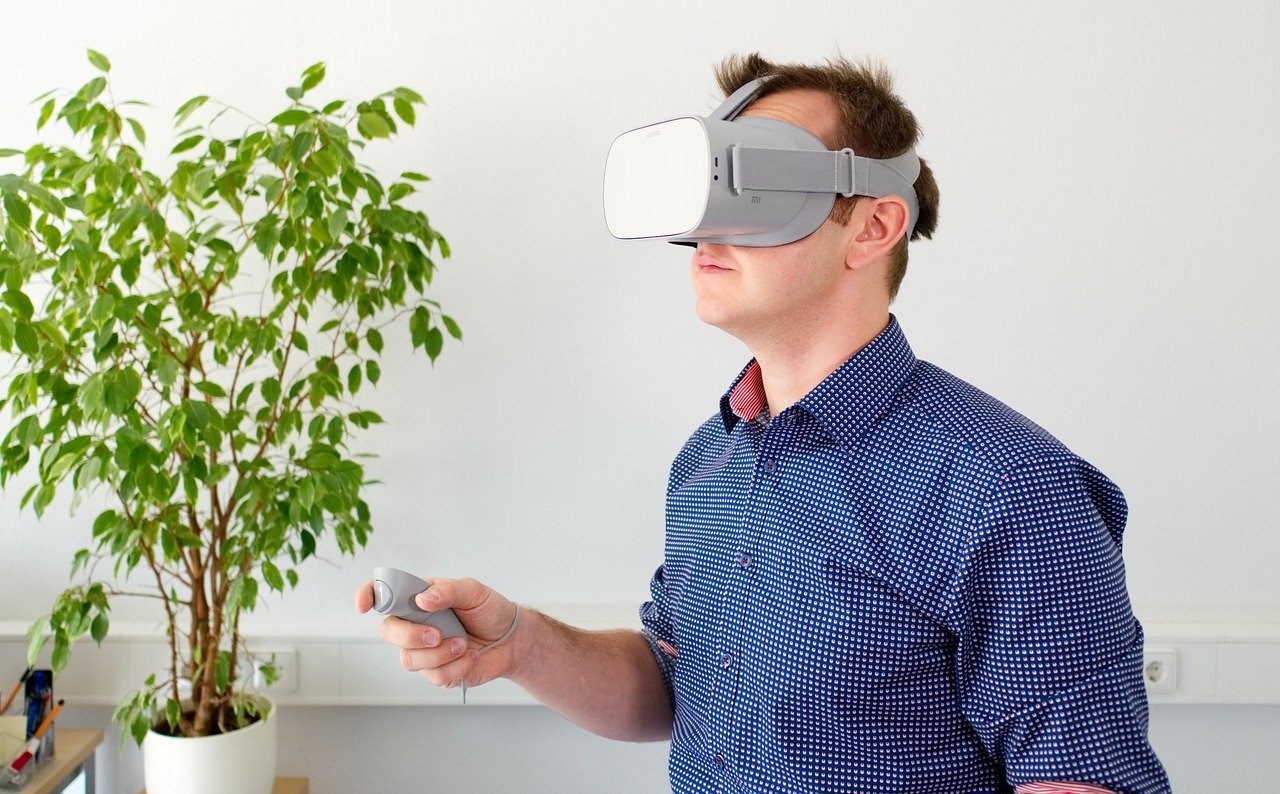
\includegraphics[scale=0.3]{img/vr-brille.jpg}
          \caption[Autarke VR-Brille mit 3D-Eingabegerät von Oculus.]{Autarke VR-Brille mit 3D-Eingabegerät von Oculus. [Quelle: \url{https://pixabay.com}].}
          \label{fig:vr-brille}
        \end{figure}
        Diese sind mittlerweile sehr kompakt,
        leistungsstark und finanziell erschwinglich. Dadurch, dass Hardware kleiner
        und günstiger wird, kann der Trend beobachtet werden, dass VR-Brillen auch ohne
        einen stationären Computer leistungsstark sind.
        Der Vorteil von VR-Brillen, im Gegensatz zu Projektionssystemen, bildet die 
        Möglichkeit, diese überall tragen und nutzen zu können [\cite[129]{Dorner2013}].
        Dementsprechend haben sich Head-Mounted-Displays als VR-Systeme auf dem Massenmarkt
        durchgesetzt, da diese kompakt sind und nicht zwingend einen Computer benötigen.
        Zudem ist je nach Anwendungsfall eine VR-Brille nicht notwendig, da moderne 
        mobile Endgeräte, wie Smartphones, bereits genügend Leistung für eine 
        Echtzeit-Simulation mitbringen. So gibt es Aufsätze für das Smartphone,
        mit welchen sich dieses in eine VR-Brille umfunktionieren lässt (siehe Abb. \ref{fig:google-cardboard}).
        Da diese Lösung kostengünstig und einfach umzusetzen ist, stellt dies eine
        gute Einstiegsmöglichkeit für Personen dar, die gerne
        VR-Erfahrungen erleben, sich jedoch nicht eine hochwertige VR-Brille leisten
        möchten.
        \begin{figure}[t]
          \centering
          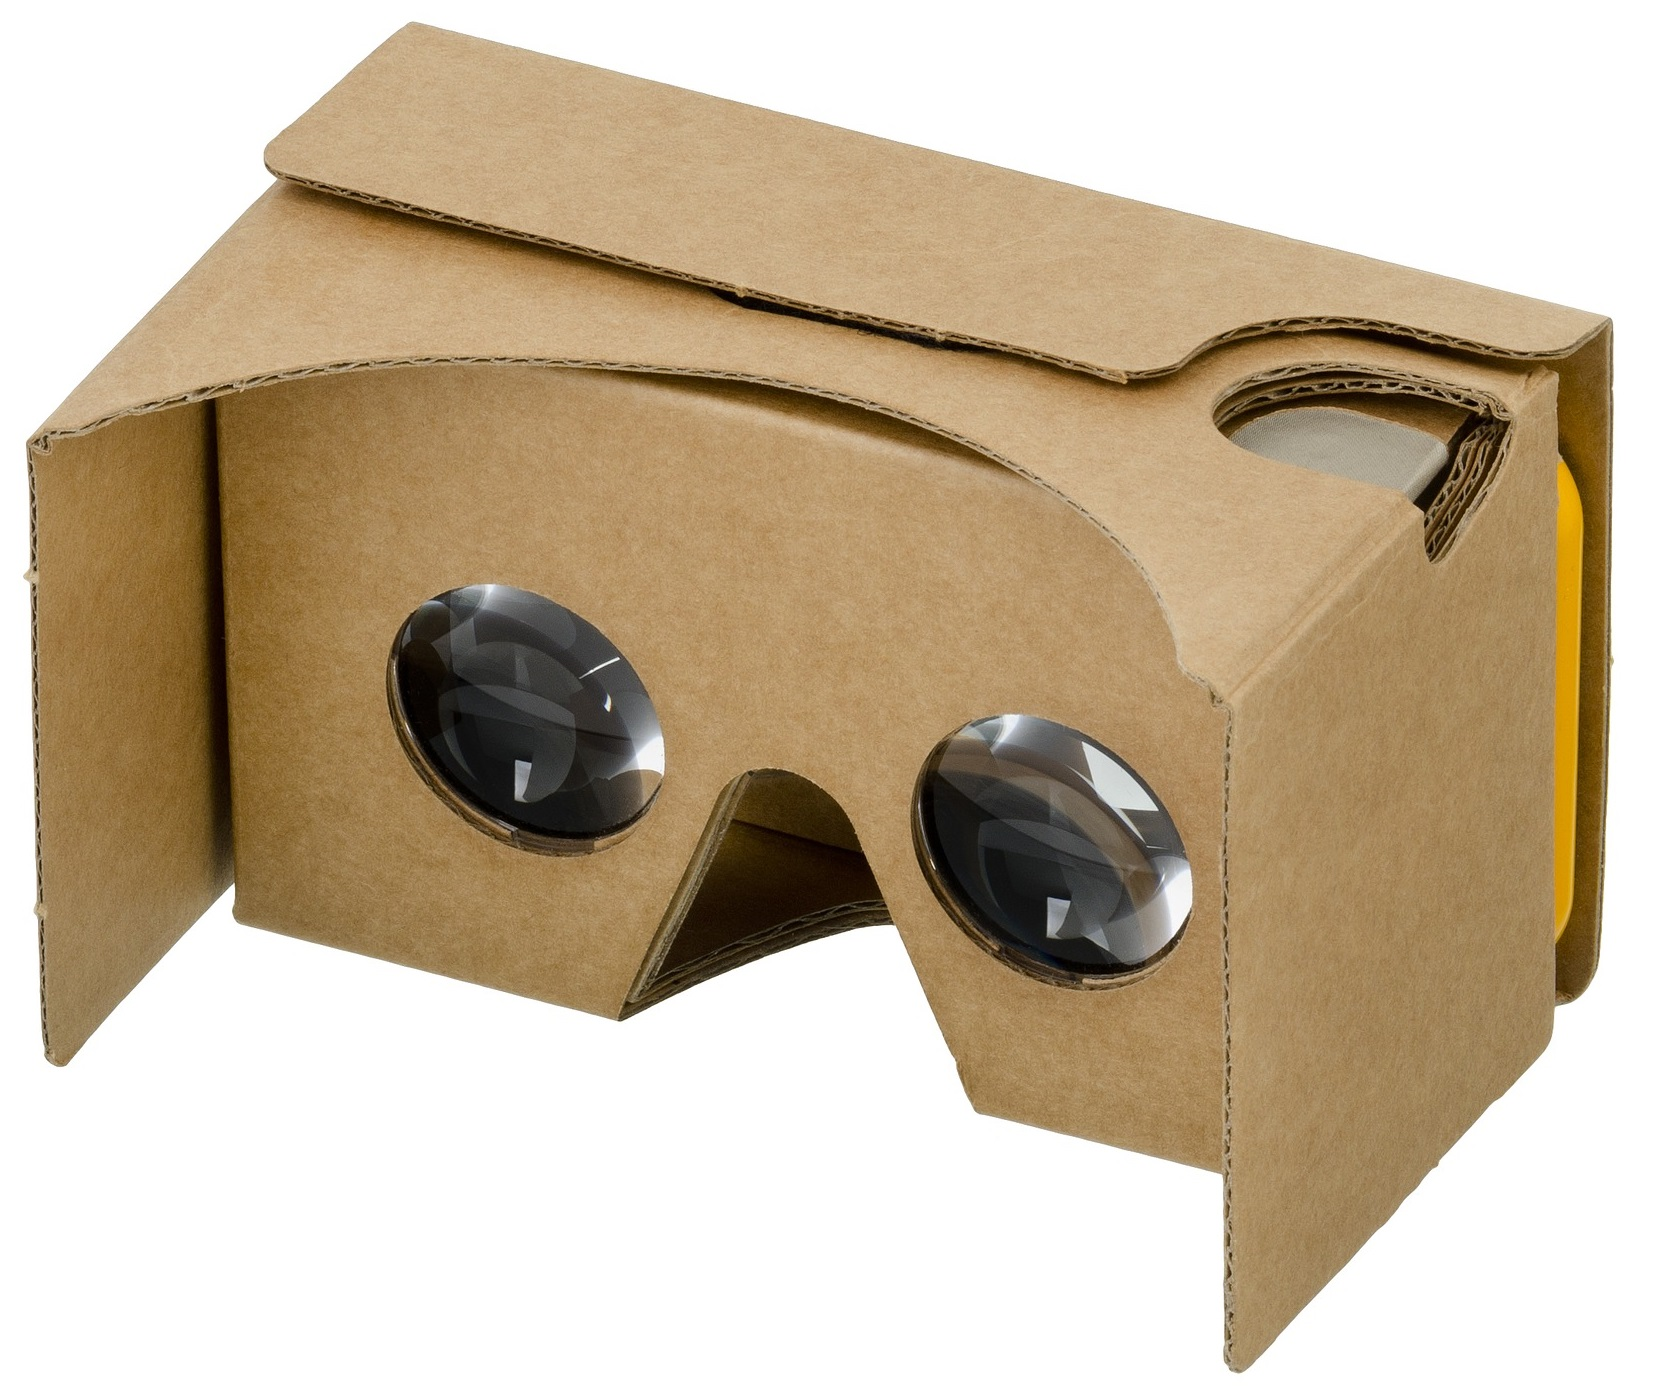
\includegraphics[scale=0.7]{img/google-cardboard.jpg}
          \caption[Google Cardboard für Smartphones.]{Google Cardboard für Smartphones. [Quelle: \url{https://pixabay.com}].}
          \label{fig:google-cardboard}
        \end{figure}
        Doch ist durch das Fehlen der 3D-Eingaberäte bei dieser Lösung, je
        nach Anwendungsfall, eine Einschränkung festzustellen. Abhängig von dem 
        jeweiligen Smartphone kann 
        auch eine geringe
        Bildschirmauflösung die in Kapitel \ref{Wahrnehmungsaspekte} genannten Aspekte
        beinträchtigen und einen Bruch der Illusionen hervorrufen.
        Projektionssysteme, die die simulierte Umgebung auf ganzen Leinwänden darstellen,
        haben den Vorteil, dass sich der Benutzer nicht unmittelbar vor dem Bildschirm
        befindet [\cite[134]{Dorner2013}]. Dadurch können keine einzelnen Pixel mit dem Auge 
        erfasst werden. \\ \\ \\ \\
        Aktuelle Unternehmen, die sich mit VR-Brillen beschäftigen und diese Technologie
        maßgeblich vorgeben, sind unter anderem Facebook mit Oculus\footnote{Oculus | \url{https://www.oculus.com/} (22.11.2020).}, 
        HTC mit Vive\footnote{HTC VIVE | \url{https://www.vive.com/de/} (22.11.2020).},
        Playstation mit PlaystationVR\footnote{PlaystationVR | \url{https://www.playstation.com/de-de/explore/playstation-vr/} (22.11.2020).}
        und Valve Corporation mit der Valve Index\footnote{Valve Index | \url{https://www.valvesoftware.com/de/index/headset} (22.11.2020).}.
        Samsung beschäftigt sich ebenfalls mit Virtual
        Reality, jedoch bieten diese nur eine hochwertige Brille ohne Rechenleistung an.
        Für den vollständigen Funktionsumfang wird zusätzlich ein Samsung Smartphone vorausgesetzt\footnote{Samsung Gear VR | \url{https://www.samsung.com/de/wearables/gear-vr-r323/} (22.11.2020).}.
        Auch Nintendo hat mit der Konsole Nintendo Switch den Weg zu Virtual Reality
        gefunden\footnote{Nintendo Labo VR-SET | \url{https://www.nintendo.de/Nintendo-Labo/Nintendo-Labo-1328637.html} (22.11.2020).}.
        Das VR-Set für die Nintendo Switch bietet sich hilfreich für Kinder an, um erste 
        Erfahrungen mit Virtual Reality machen zu können.
        Auch Google ist mit dem Google Cardboard in diesen Markt involviert, bietet jedoch keine 
        VR-Brille mit integrierter Hardware an.
      \subsubsection{Native und webbasierte Anwendungen}
        Es gibt zahlreiche Software-Development-Kits (SDK).
        VR-Anwendungen können heutzutage mit Hilfe von unterschiedlichen Programmen oder Frameworks entwickelt
        werden. So kann ein Produkt nativ für eine Plattform entwickelt werden oder durch
        webbasierte Anwendungen plattformunabhängig funktionieren.
        Beide Ansätze bieten ihre Vor- sowie Nachteile und sind daher vom jeweiligen 
        Anwendungsfall abhängig. \\ \\
        Native Lösungen bieten eine geeignetere
        Performanz, da diese Anwendungen mit Programmiersprachen entwickelt werden die
        effizient und maschinennah sind. Je nach Hersteller gibt es auch für das 
        Betriebssystem eigene Programmiersprachen, die dann für das jeweilige Ökosystem 
        optimiert werden können. \\
        Webanwendungen, die meist auf der Basis von JavaScript laufen, werden nicht 
        kompiliert sondern interpretiert und der Quellcode wird zur Laufzeit vom Browser 
        gelesen und ausgeführt. Und das bei jeder Ausführung des Codes.
        Durch eine große und aktive Community hat sich JavaScript in den letzten Jahren 
        zu einer universellen Programmiersprache entwickelt und findet Anwendung in
        fast allen Gebieten der Softwareentwicklung.
        Diese Entwicklung der letzten Jahre hat gezeigt, dass der Mensch weniger
        Zeit vor dem Computer oder Laptop im Internet verbringt, sondern hauptsächlich mobil auf das Netz zugreift 
        [\cite[1]{Ater2017}].
        Durch das Betrachten von Internetseiten auf einem mobilen Endgerät wurde der
        Ansatz mobile-first immer wichtiger [\cite[1]{Ater2017}]. Die Vorteile, die native
        Anwendungen mehrere Jahre mit sich brachten, waren, neben der besseren Leistung,
        erweiterte Grafikmöglichkeiten, Standortermittlung, Push-Benachrichtigungen,
        Offlineverfügbarkeit und Startbildschirm-Verknüpfungen [\cite[3]{Ater2017}]. Diese
        Funktionen waren damals notwendig für erfolgreiche Apps, da diese dem
        Benutzer eine bessere Nutzungserfahrung ermöglichten. 
        Heutzutage hat sich das Web als Plattform weiterentwickelt, sodass jene Funktionen nicht
        mehr nur nativen Anwendungen vorenthalten sind.
        Sogenannte Progressive Web Apps können sich an nativen Funktionen der Plattform zu
        bedienen, bieten jedoch weiterhin die Flexibilität, die das Web mit sich bringt
        [\cite[2]{Ater2017}].
        So können webbasierte Anwendungen offlinefähig gestaltet werden. Darüber hinaus können
        Push-Benachrichtigungen von Webseiten verschickt werden und es lassen sich
        Desktop- und Startbildschirmverknüpfungen über moderne Browser anlegen [\cite[5-6]{Ater2017}].
        Durch das Ausblenden der URL-Leiste des Browsers
        und das Ausführen der webbasierten Anwendung im Vollbildmodus, ähneln sie den
        nativen Anwendungen in ihrem Funktionsumfang und ihrer Erscheinung [\cite[6]{Ater2017}]. 
        Für das Ziel eine Anwendung
        möglichst zugänglich zu machen, ist die Entwicklung einer webbasierten Lösung
        vorteilhaft, da plattformunabhängig entwickelt werden kann und der
        Benutzer direkt am Ziel ist, sobald dieser die Webseite öffnet.
        Es muss kein zusätzlicher
        Download oder eine zusätzliche Installation erfolgen und auch das Pflegen mehrerer
        Versionen in den verschiedenen App Stores entfällt. So kann der Benutzer unabhängig
        von Plattform und seinem Gerät die Anwendung benutzen. Da der Benutzer 
        demnach an keine Plattform
        gebunden ist, lässt sich die Reichweite um ein vielfaches skalieren [\cite[3]{Ater2017}].
        Es ist zunehmend schwieriger geworden Benutzer für den Download einer App 
        zu motivieren [\cite[3]{Ater2017}].
        Die meisten Benutzer gehen bereits auf dem Weg zum jeweiligen Store und der darauffolgenden
        Installation verloren [\cite[4]{Ater2017}]. Application Programming Interfaces (API) 
        wie die Web Share und Web Share Target
        API sind nur ein Teil der zukünftigen Entwicklung, die immer mehr Funktionen ins
        Web bringen, welche zuvor lediglich für native Anwendungen zur Verfügung standen [\cite[245]{Ater2017}]. \\
        So findet auch Virtual Reality, durch die WebXR-Schnittstelle (ehemals WebVR),
        Anwendung im Browser [\cite[245]{Ater2017}]. In Kombination mit WebGL lassen sich komplexe,
        rechenintensive und überzeugende VR-Erfahrungen entwickeln [\cite[245]{Ater2017}].
        Die Schnittstelle WebXR ist kompatibel mit allen der heutigen im Handel erhältlichen
        VR-Brillen und kann auch
        ihre jeweiligen 3D-Eingabegeräte lesen, wodurch der Entwickler Zugang zu allen Informationen
        bekommt, die auch eine native Desktop-Anwendung mitbringen würde [\cite[245]{Ater2017}].
        Im Punkt Leistung sind nach wie vor native Anwendungen einige Schritte voraus, doch
        gibt es bereits Ansätze dieses Problem zu beheben. WebAssembly\footnote{WebAssembly Webseite | \url{https://webassembly.org/} (22.11.2020).}
        ist eine niedere Programmiersprache, welche wenig Abstraktion zur Befehlssatzarchitektur
        des Computers bietet [\cite[185]{Haas2017Jun}]. Dadurch, dass WebAssembly zu ByteCode
        kompiliert wird, kann näherungsweise die native Leistung mit einer webbasierten Anwendung 
        erreicht werden [\cite[186]{Haas2017Jun}]. 
        Plattformunabhängigkeit bleibt geboten,
        da WebAssembly über den Browser ausgeführt werden kann.
        Jedoch ist WebAssembly nicht
        so verbreitet wie JavaScript und bietet deshalb weniger Technologien und Möglichkeiten,
        zur Entwicklung von VR-Anwendungen. Zum aktuellen Zeitpunkt bietet die Unity Engine
        die Möglichkeit, VR-Anwendungen mit Hilfe ihrer Engine zu entwickeln und
        diese für moderne Browser in WebAssembly (in Kombination mit JavaScript) 
        zu exportieren\footnote{WebAssembly in Unity | \url{https://blogs.unity3d.com/2018/08/15/webassembly-is-here/} (22.11.2020).}.
        Die Unreal Engine kompiliert den geschriebenen Code ebenfalls zu WebAssembly,
        hat die HTML5-Entwicklung jedoch als Erweiterung ausgelagert, die durch
        die Community weiterentwickelt werden soll\footnote{Unreal Engine Dokumentation für HTML5 Development | \url{https://docs.unrealengine.com/en-US/Platforms/HTML5/index.html} (22.11.2020).}.
        Da es in der klassischen Softwareentwicklung nicht sinnvoll ist in Assemblersprache
        zu entwickeln, da dies zu komplex und zeitaufwendig wäre, 
        macht es ebenfalls wenig Sinn selbstständig eine VR-Anwendung in 
        WebAssembly zu entwickeln. Deshalb wird eine Programmiersprache benötigt, die
        eine höhere Abstraktion bietet. So ist es angebracht Unity oder Unreal Engine 
        als Software zu verwenden,
        um VR-Anwendungen auf Basis von WebAssembly zu generieren.
        Die Frage, ob nativ oder für das Web entwickelt werden soll, 
        ist abhängig vom Anwendungsfall. \\
        Für das Cranach Digital Archive bietet sich eine webbasierte Lösung
        an, da die Darstellung von Gemälden und Archivalien keine hochkomplexen Berechnungen
        benötigt. Das aktuelle Archiv ist über das Internet zu erreichen und lässt sich auf
        Desktop-PCs und mobilen Endgeräten betrachten, dementsprechend 
        sollte die VR-Lösung ebenfalls
        über das Web zugänglich sein. So können auch Kunstinteressierte, die sich keine hochwertige
        VR-Brille leisten möchten, die Gemälde und Archivalien mit ihrem Smartphone
        virtuell erkunden. \\
        Durch eine plattformunabhängige Lösung ist weniger Wartung notwendig und das
        Bereitstellen in die jeweiligen App Stores entfällt, sodass zeitlicher Aufwand und
        Ressourcen gespart werden können [\cite[248]{Ater2017}]. Webbasierte Anwendungen 
        benötigen die wenigsten Ressourcen für eine hohe Zugänglichkeit, wodurch sich dieser
        Entwicklungsansatz auch für das Forschungsprojekt anbietet.
    \subsection{Virtual Reality im musealen Kontext}
      Die Idee Kunst in einer virtuellen Realität darzustellen, ist keine neue Idee.
      Immer wieder wagten sich Museem daran, stellten Konzepte auf, sammelten
      Erfahrungsberichte und entwickelten eigene Produkte [\cite{Heidsiek2019}]. Es ist
      ein wichtiger und sinnvoller Schritt, dass Virtual Reality
      im musealen Bereich vermehrt und umfangreich Anwendung findet. Museen versuchen
      primär Wissen, Erfahrungen sowie Emotionen zu übermitteln und 
      durch den Einsatz von Virtual Reality
      besteht die Möglichkeit, den Besucher in Szenarien zu versetzen, die in der
      Vergangenheit geschehen sind. Der Besucher kann auch Fantasiewelten der Künstler
      wahrnehmen, um ein besseres Verständnis für ihre Kunst zu erlangen. Umfragen ergaben, 
      dass ein generelles Interesse an neuartigen Technologien im Museum vorhanden ist [\cite[34]{Heidsiek2019}].
      Die Besucher erhoffen sich dadurch, dass Museen unterhaltsamer, lehrreicher und
      zugänglicher werden [\cite[34]{Heidsiek2019}]. Gerade Virtual Reality lässt Museen
      und Informationen für die breite Masse zugänglicher werden, denn die Besucher 
      sind nicht mehr gezwungen 
      das Museum physisch zu besuchen. \\
      Der Anwendungsbereich ist vielfältig und die 
      Technologie noch nicht ausgereizt.
      Doch birgen neue Technologien neben ihren Chancen auch Risiken, die berücksichtigt
      und disktutiert werden müssen. In diesem Kapitel wird auf die
      Risiken und auch auf die Chancen eingegangen, die ein Einsatz von
      Virtual Reality mit sich bringen kann. Da das Cranach Digital Archive nicht das erste Museum ist, 
      welches Kunst digitalisiert, sollen bereits entwickelte Produkte analysiert
      werden, deren Erkentnisse und Ideen dabei helfen, bereits begangene Fehler zu 
      vermeiden und geeignete Prototypen zu entwickeln.
      \subsubsection{Chancen und Risiken}
        Museen sind Stätten des Wissens. Ihre Aufgabe besteht darin, Menschen Wissen zu
        vermitteln, dies meist über vergangene Erfahrungen oder Geschehnisse [\cite[24]{fischer2001}].
        Durch die Digitalisierung und das Internet war es erstmals möglich, historische Gegenstände
        oder Gemälde mit der ganzen Welt zu teilen, unabhängig des Standortes eines
        Betrachters. Dementsprechend liegt der Mehrwert von digitalen Museen darin, eine
        erhöhte Vervielfältigung und Verbreitung von Wissen bereit zu stellen [\cite[17]{Huennekens2002}].
        Auch das Anwendunsgebiet Virtual Reality bietet in Verbindung mit dem Internet und der Digitalisierung
        eine neue Möglichkeit Informationen innovativ zu übermitteln [\cite[52]{Heidsiek2019}]. \\
        So wird das Museum als Stätte des Wissens effizienter gestaltet und ermöglicht 
        mehr Menschen
        zu erreichen, als es vorher möglich war. Das Cranach Digital Archive geht hier mit
        gutem Beispiel voran und bietet eine umfangreiche Datenbank
        zu den Werken und Archivalien der Cranachs.
        Im Vergleich zu statischen Objekten, wie an Wänden hängenden Gemälden, lassen sich 
        durch digitale Lösungen verschiedene und neue Darstellungen ermöglichen [\cite[17]{Huennekens2002}].
        Besonders Virtual Reality bietet hier eine sehr interessante Möglichkeit, völlig neue
        Perspektiven zu erschaffen, die in der realen Welt nicht erreicht werden können. \\
        Ein Vorteil in Virtual Reality liegt darin, dass die Gesetze von Raum und Zeit nicht
        in einer virtuellen Realität gelten [\cite[140]{Huennekens2002}]. So kann der Mensch
        seinem Bedürfnis, alltägliche Erfahrungen zu überschreiten, nachkommen [\cite[140]{Huennekens2002}].
        Diese Möglichkeiten bringen jedoch auch eine ethische 
        Verantwortung zur Präsentation musealer Gegenstände mit sich.
        Das Loslösen von Raum und Zeit kann sich negativ auf die historischen Inhalte auswirken
        [\cite[141]{Huennekens2002}]. Durch eine falsche Darstellung könnte 
        sogar von Entweihung der historischen
        Gegenstände gesprochen werden [\cite[141]{Huennekens2002}]. Deshalb liegt es in der 
        Verantwortung der
        Museen die historische Integrität eines Gegenstandes oder einer Erfahrung nicht
        zu verletzen [\cite[38]{Heidsiek2019}]. Dies kann vermieden werden, indem 
        kenntlich gemacht wird, was original ist und was nachträglich hinzugefügt
        wurde [\cite[38]{Heidsiek2019}]. Sobald virtuelle Realitäten erfundene Aspekte 
        beinhalten, und diese nicht als solche gekennzeichnet wurden, handelt es sich nicht
        mehr um eine historische Überlieferung, sondern um persönliche und subjektive 
        Wahrnehmungen [\cite[38]{Heidsiek2019}]. Fotorealistische Darstellungen
        von unwahren Ereignissen oder Objekten können verstärkt dazu führen, dass der
        Benutzer von einer fälschlichen Tatsache überzeugt wird [\cite[39]{Heidsiek2019}].
        So hat jedes Museum, dass Virtual Reality als Möglichkeit zur Betrachtung 
        kunstrelevanter Objekte anbieten möchte, die ethische Verantwortung, 
        dem Benutzer zu jedem Zeitpunkt kenntlich zu machen,
        was eine historische Übermittlung und was virtuelle Realität ist. \\
        Zudem besteht durch Virtual Reality die Gefahr, dass Museen, auf lange Sicht 
        betrachtet, obsolet werden und alles über eine VR-Brille erforscht werden kann
        [\cite[142-143]{Huennekens2002}]. Besucher die Virtual Reality in Museen genutzt
        haben, betrachten diese Technologie jedoch als Ergänzung zum Museum und nicht als
        haben, betrachten diese Technologie jedoch als Ergänzung zum Museum und nicht als
        einen vollständigen Ersatz, da der Hauptgrund eines Museumsbesuchs die Betrachtung
        der Originalobjekte sei [\cite[79]{Heidsiek2019}]. Originale Ausstellungsstücke
        haben demnach weiterhin einen nicht reproduzierbaren Charakter, welcher sich nicht 
        durch eine
        virtuelle Realität darstellen lässt [\cite[93]{Heidsiek2019}]. So schwächt die
        Darstellungen von Originalobjekten als Kopie in einer virtuellen Welt
        die Authentizität dieser [\cite[93]{Heidsiek2019}]. 
        Besucher, die vorher eine Online-Ausstellung eines Museums gesehen haben,
        entschieden sich sogar aufgrund dessen für das Besuchen des Museums in der 
        realen Welt [\cite[777-778]{Katz2015}]. So kann eine VR-Erfahrung, die über
        das Web zu erreichen ist, nicht als Ersatz für das Museum gesehen werden,
        sondern auch als innovatives und modernes Marketingwerkzeug.
        Dementsprechend ist nach aktuellem
        Stand nicht davon auszugehen, dass die Technologie Virtual Reality das Museum in
        naher oder mittlerer Zukunft obsolet macht.
        Die Museumslandschaft sieht in Virtual Reality die Chancen, neue und andere
        Geschichten zu vermitteln, langfristig für Besucher attraktiv zu bleiben und
        auch eine neue Zielgruppe zu erreichen [\cite[34-35]{Heidsiek2019}]. \\
        Da Emotionen Teil eines Museumsbesuchs sind, lassen sich durch den Einsatz
        von Virtual Reality neue und intensivere Emotionen hervorrufen.
        So konnte nachgewiesen werden, dass VR-Erfahrungen
        bei musealen Ausstellungen zu erhöhtem Interesse, erhöhter Zufriedenheit und 
        Vergnügen geführt haben [\cite[69-72]{Heidsiek2019}]. Dadurch können schwer
        verständliche Themen leichter übermittelt werden und der Informationsaustausch
        zwischen Museum und Mensch optimiert werden. 
        Im Zuge dessen entsteht die Möglichkeit langfristig für Besucher 
        attraktiv zu bleiben und eine neue Zielgruppe anzusprechen,
        die vorher kein gesteigertes Interesse an einem Museumsbesuch besaßen.
        Aber auch die aktuelle Zielgruppe eines Museums, unabhängig des Alters, kann
        etwas mit Virtual Reality anfangen und ist nicht abgeneigt zu dieser Technologie [\cite[75]{Heidsiek2019}].
      \subsubsection{Optimierung des Lernprozesses} \label{Optimierung des Lernprozesses}
        Empfundene Emotionen steigern bei einem Lernprozess nachweislich 
        den erhöhten Lernerfolg [\cite[29]{Heidsiek2019}].
        Um diese Emotionen bei Besuchern zu aktivieren und entsprechende
        Gefühle hervorzurufen, bietet es sich an, Lebensräume der darzustellenden Personen
        oder Objekte in der virtuellen Welt nachzustellen [\cite[35-36]{Heidsiek2019}].
        Anhand dessen kann sich der Benutzer noch besser in die Situation hineinbegeben
        und komplexe Gefühle und Emotionen besser wahrnehmen. Storytelling stellt hierbei
        eine mögliche Methode dar [\cite[35-39]{Heidsiek2019}].
        Bei VR-Erfahrungen im Museum lassen sich zwei Emotionen beobachten: 
        Die erfahrungsbezogene und inhaltsbezogene Emotion [\cite[69]{Heidsiek2019}]. 
        Erstere beschreibt die
        empfundene Emotion, die während der gesamten Nutzungserfahrung entstanden ist und
        letztere die Emotion, die empfunden wird, während sich mit einem genauen
        Ausstellungsstück beschäftigt wird. Virtual Reality ruft vermehrt die 
        erfahrungsbezogenen Emotionen hervor [\cite[69]{Heidsiek2019}], was im Hinblick auf
        die Technologie nachvollziehbar erscheint. Denn durch Virtual Reality liegt der
        Fokus nicht nur auf genau einem einzigen Objekt, sondern meist auf einer ganzen
        Szene und die Erfahrung innerhalb dieser. Die erfahrungsbezogenen Emotionen 
        sind diejenigen, die einen besseren
        Lerneffekt mit sich bringen, sodass Museen dadurch als unterhaltsamer und
        aufregender wahrgenommen werden [\cite[69]{Heidsiek2019}]. Traditionelle Museen rufen 
        hauptsächlich inhaltsbezogene Emotionen hervor [\cite[69]{Heidsiek2019}], da der
        Fokus bei Ausstellungen oft auf einzelnen Ausstellungsstücken liegt.
        Immersive Umgebungen, die Virtual Reality in hoher Form bieten kann, tragen ebenfalls
        zu einem optimierten Lernprozess bei, da der Lernende den Inhalt selbstständig steuern
        und manipulieren kann [\cite[777]{Katz2015}]. Ebenso kann der Lernende
        die Lerngeschwindigkeit eigenmächtig bestimmen [\cite[777]{Katz2015}],
        was die Konzentration erhöht. Nichtsdestotrotz muss berücksichtigt werden,
        dass nicht jeder Anwender sofort perfekt mit der virtuellen Umgebung agieren
        kann. So kann durch zu komplizierte Interaktionen und Darstellungen
        eher eine negative Erfahrung hervorgerufen werden, die dem Lernprozess eher
        schadet [\cite[777]{Katz2015}]. An dieser Stelle ist die
        Studie des Deutschen Auswandererhauses zu erwähnen, welche eine einfache
        Bedienung durch blickgesteuerte Interaktion gewährleistet [\cite[38]{Heidsiek2019}].
        Durch das Fehlen von Eingabegeräten müssen die Benutzer lediglich 
        eine Brille aufsetzen und können
        sofort innerhalb der Anwendung navigieren, da keine Knöpfe
        auswendig gelernt werden müssen.
        Auch das Gefühl der Präsenz, welches bereits in Kapitel \ref{Wahrnehmungsaspekte}
        behandelt wurde, trägt dazu bei, wie gut der Lernende Informationen aufnimmt
        [\cite[777]{Katz2015}].
      \subsubsection{Aktuelle Lösungen und Umsetzung} \label{Aktuelle Lösungen und Umsetzung}
        Da es viele unterschiedliche Technologien und Hardware für die Umsetzung von 
        VR-Ausstellungen 
        gibt, lassen sich auch viele verschiedene Wege nutzen, VR-Erfahrungen 
        zu entwickeln. \\
        Das Deutsche Auswandererhaus beispielsweise entschied sich für das Samsung Odyssey
        Virtual Reality Headset, welches ohne Controller genutzt werden kann und intuitiv
        bedienbar ist [\cite[35]{Heidsiek2019}]. Sie entwickelten eine VR-Erfahrung, die
        durch Storytelling vermittelt wurde [\cite[35-39]{Heidsiek2019}]. Dabei
        konnten zwei VR-Erfahrungen erlebt werden. Eine der beiden bestand aus einer 
        auditiven und
        blickgesteuerten Interaktion, während sich die Andere aus 
        einem 360-Grad-Video zusammensetzte [\cite[38]{Heidsiek2019}]. Beide Varianten
        erzählten die Geschichte eines Kriegsgefangenen.
        Aufgrund der positiven Studienergebnisse und Bewertungen der Probanten, scheint
        die Entwicklung einer VR-Erfahrung mit blickgesteuerter Interaktion sinnvoll, da
        keine Einarbeit in die Eingabegeräte der VR-Brille notwendig ist. Dadurch erhält
        die Anwendung eine intuitive Steuerung und das Vermitteln einer Geschichte 
        innerhalb der VR-Erfahrung fördert das Interesse der Benutzer [\cite[35-39]{Heidsiek2019}]. \\
        Google bietet ebenfalls eine simple Anwendung, die über ein Google Daydream\footnote{VR-Brille von Google | \url{https://arvr.google.com/daydream/} (22.11.2020).}
        kompatibles Smartphone ausgeführt werden kann\footnote{Google Arts \& Culture VR | \url{https://play.google.com/store/apps/details?id=com.google.vr.museums&hl=de} (22.11.2020).}.
        Hierbei lassen sich Gemälde aus verschiedenen Perspektiven betrachten.
        Besondere Funktionen oder ein Storytelling weist diese App nicht auf. Sie immitiert
        letztlich einen Museumsbesuch in einer virtuellen Welt. \\ \\ \\
        Das Archäologische Museum in Hamburg bietet ebenfalls einen Rundgang durch
        das Museum in 3D und Virtual Reality an\footnote{Archäologisches Museum Hamburg | \url{https://amh.de/digitales-angebot/google-art-project/} (22.11.2020).}.
        Dabei handelt es sich um eine Webanwendung, welche mit einem Smartphone und
        Google Cardboard erkundet werden kann. Wer eine vollwertige VR-Brille besitzt,
        unabhängig vom Hersteller, kann dieses VR-Erlebnis ebenfalls über einen VR-Browser
        erfahren. Somit spricht das Archäologische Museum Hamburg die größtmögliche 
        Nutzerzahl an.
        Die Umsetzung ist relativ simpel, da es sich um eine einfache Museumsrundführung
        ohne bestimmte Funktionen handelt. \\
        Das Deutsche Museum in München bietet ein VRlab an, in dem Besucher in die Vergangenheit
        reisen und dort mit Objekten interagieren können\footnote{Deutsches Museum | \url{https://www.deutsches-museum.de/ausstellungen/sonderausstellungen/vrlab/} (22.11.2020).}.
        Auch eine Fahrt über den Mond ist möglich. Das Deutsche Museum in München 
        zeigt an dieser Stelle,
        dass die Möglichkeiten von Virtual Reality vor allem zur Erkundung physikalisch unmöglicher
        Szenarien genutzt werden sollten. An 
        diesem Beispiel lässt sich gut erkennen, dass Virtual Reality nicht als Ersatz, sondern
        als Ergänzung zu einem klassischen Museumsbesuch genutzt werden kann. \\
        Das Städel Museum bietet auch eine Zeitreise an, mit der das Museum im 19. Jahrhundert
        betrachtet werden kann\footnote{Zeitreise Städel Museum | \url{https://zeitreise.staedelmuseum.de/vr-app/} (22.11.2020).}.
        Die Anwendung wurde in Kooperation mit Samsung entwickelt, weshalb die App
        nur mit einem Samsung Smartphone oder einer VR-Brille von Oculus betrachtet werden
        kann. Hierdurch schränkt das Städel Museum seine Zielgruppe enorm ein. 
        Darüber hinaus bieten sie den Benutzern, durch das Veröffentlichen der App
        in einem Store, die Möglichkeit, die Erfahrung auch von zu Hause aus zu erleben. \\
        Eine weitere Möglichkeit, um den Inhalt einer VR-Erfahrung verständlicher zu übermitteln
        ist der Einsatz von Museumsführern. Entweder durch eine einfache Vertonung 
        oder das zusätzliche Einbauen eines Avatars. 
        Virtuelle Museumsführer können nachweislich zu einem höheren
        Engagement und höherer Aufmerksamkeit des Betrachters führen, da der Inhalt
        verständlicher wird [\cite[299-300]{Carrozzino2018}].
        Den Ansatz, mit Vertonung zu arbeiten, hat das Deutsche Auswandererhaus ebenfalls in
        ihrer Studie durchgeführt.
        Soll ein ideales VR-System entwickelt werden, muss, wie in Kapitel \ref{Wahrnehmungsaspekte}
        erwähnt, auch der akustische Sinn miteinbezogen werden. Je mehr Sinne miteinbezogen
        werden, desto besser sei die VR-Erfahrung für den Benutzer.
  \section{Prototyping}
    Das Prototyping ist eine Methode in der Softwareentwicklung, um schnell und mit 
    wenig Ressourcen an Ergebnisse zu gelangen. Diese Ergebnisse ermöglichen die
    Eignung eines Lösungsansatzes und der genutzten Technologien zu bewerten. \\
    Diese Methode wird im vorliegenden Forschungsprojekt angewandt, um mehrere Ergebnise im
    Hinblick auf technische Möglichkeiten der Darstellung und Interaktion zu erzielen.
    Diese Ergebnisse können als Ansatzpunkt dienen, um eine vollwertige Software 
    in diesem Anwendungsbereich entwickeln zu können.
    Zu Beginn müssen die Anforderungen an das VR-Systems erstellt werden. Da
    das Ziel dieser Arbeit keine eindeutige Lösung fordert, sondern herausfinden möchte,
    wie solch ein System für das Cranach Digital Archive entwickelt werden kann, werden
    die Anforderungen auf Basis von Erfahrungen der bereits entwickelten Produkte und der 
    Literaturergebnisse festgelegt.
    Zunächst muss dazu eine geeignete Technologie
    gewählt werden, um eine VR-Anwendung entwickeln zu können. So werden in diesem Kapitel
    die aktuellsten und populärsten Frameworks und Librarys in Betracht gezogen und kritisch
    hinterfragt, um zu entscheiden welche sich für den 
    vorliegenden Anwendungsfall am besten eignen.
    \subsection{Anforderungen an das VR-System}
      Das aktuelle Cranach Digital Archive ist bereits eine Webanwendung und kann 
      über jedes browserfähige Gerät aufgerufen werden. Somit soll dieser Ansatz 
      der maximalen Zugänglichkeit im vorliegenden Forschungsprojekt 
      weiterhin aufgegriffen werden.
      Zudem sollte das Ziel eines Museums, dem Verbreiten von Wissen, keiner Zielgruppe
      durch die Technologieauswahl verwehrt werden.
      Deshalb ist die erste Anforderung an das VR-System die Zugänglichkeit
      über das Web als webbasierte Anwendung. \\
      Diese Anwendung, welche unter Umständen vom Benutzer auch auf einem 
      Smartphone aufgerufen wird, muss dementsprechend ohne 
      3D-Eingabegerät funktionieren.
      Darüber hinaus ist durch eine blickorientierte Steuerung die Anwendung für
      den Benutzer zugänglicher und kann daher, wie bereits in
      Kapitel \ref{Optimierung des Lernprozesses}
      und \ref{Aktuelle Lösungen und Umsetzung} erwähnt, ohne erschwerte Einarbeitung
      genutzt werden. 
      Eine solche blickorientierte Steuerung ist intuitiv und benötigt weniger
      Hardware. Dies stellt die zweite Anforderung an das VR-System dar. \\
      Um dem Benutzer eine immersive und interessante VR-Erfahrung zu ermöglichen, sollen
      möglichst viele Sinne miteinbezogen werden. In Kapitel \ref{Wahrnehmungsaspekte}
      wurde festgehalten, dass ein perfektes VR-System alle Sinne des Menschen miteinbezieht.
      Da dies aktuell technisch jedoch nicht möglich ist, sollen so viele Sinne
      wie möglich angesprochen werden. Deshalb soll, neben dem
      visuellen Sinn der bei einer VR-Erfahrung immer
      verwendet werden muss, zusätzlich der akustische Sinn angesprochen werden.
      Das Cranach Digital Archive ist neben kunstinteressierten Benutzern auch für
      Forscher und Mitarbeiter des Teams zugänglich. In diesem Kontext soll der
      Fokus der Prototypen nicht nur auf den visuell schönen VR-Erfahrungen liegen,
      sondern auch auf der Verbesserung des generellen Datenverständnisses.
      Wie bereits in Kapitel \ref{Konzept und Nutzung von VR}
      erwähnt wurde, kann Virtual Reality dabei helfen, komplexe Datenstrukturen besser
      zu verstehen. \\ \\
      Demnach gibt es zwei Arten von VR-Systemen: Jene die für die 
      Zielgruppe eines Museums entwickelt werden und sich daher auf immersive 
      und visuell ansprechende VR-Erfahrungen fokussieren 
      und Andere, die versuchen das Verständnis für die Daten zu verbessern. 
      Jedoch ist zu erwähnen, dass beide Ansätze der VR-Systeme auch von
      beiden Zielgruppen angenommen werden können. So kann die Zielgruppe eines Museums 
      ebenfalls das Bedürfnis für ein besseres Verständnis der Daten empfinden. \\
      Die in Tabelle \ref{tab:anforderungen} verzeichnete Auflistung fasst
      alle Anforderungen der zu entwickelnden VR-Systeme zusammen.
      \begin{table}[h]
        \begin{center}
          \begin{tabular}{| c |}
            \hline
            \textbf{Die Anforderungen} \\ \hline
            Webbasierte Anwendung \\ \hline
            Blickorientierte Steuerung \\ \hline
            Bezug auf den akustischen Sinn \\ \hline
            Zielgruppenvielfalt \\ \hline
          \end{tabular}
          \caption[Anforderungen an die zu entwickelnden Prototypen.]{Anforderungen an die zu entwickelnden Prototypen. [Quelle: Eigene Darstellung].\label{tab:anforderungen}}
        \end{center}
      \end{table}
    \subsection{Analyse der Technologien}
      In diesem Kapitel werden die Vor- und Nachteile der einzelnen Frameworks, Librarys
      oder Softwares gegenübergestellt, die zur Umsetzung des Forschungsprojektes genutzt
      werden sollen. Anhand der zuvor aufgelisteten Anforderungen sowie der vorhandenen
      Ressourcen dieses Projektes wird eine entsprechende Technologielösung 
      ausgewählt.
      Die Technologien werden durch eine einfache Internetrecherche
      über WebVR herausgearbeitet.
      Damit eine Technologie in Betracht gezogen werden kann, muss diese eine gewisse
      Verbreitung und Community mit sich bringen, denn Software, die regelmäßig erweitert
      und von einer Community unterstützt wird, bringt viele Vorteile mit sich. 
      Durch die umfangreiche Nutzung einer Community ist es einfacher Lösungen
      für auftretende Entwicklungsprobleme zu finden. Zudem fördert eine große
      Anzahl bereits geschriebener Code-Pakete die Entwicklung des vorliegenden 
      Forschungsprojektes. \\
      Unity\footnote{Unity | \url{https://unity.com/de} (22.11.2020).} und 
      Unreal Engine\footnote{Unreal Engine | \url{https://www.unrealengine.com/en-US/} (22.11.2020).} 
      sind Softwarelösungen, hinter welchen zwei große
      Firmen stehen, die diese weiter entwickeln. Beide Spiele-Engines bieten eine
      große Community, eine ausführliche Dokumentation\footnote{Unreal Engine Dokumentation | \url{https://docs.unrealengine.com/en-US/index.html} (22.11.2020).\\Unity Dokumentation | \url{https://docs.unity3d.com/Manual/index.html} (22.11.2020).}
      und werden in die Auswahl der Technologie miteinbezogen. \\
      Ein weiteres populäres Framework ist React 360\footnote{React 360 | \url{https://facebook.github.io/react-360/} (22.11.2020).}
      (8.400 Stars auf GitHub\footnote{React 360 auf GitHub | \url{https://github.com/facebook/react-360} (22.11.2020).})
      und wird von Facebook entwickelt. 
      Zusätzlich zu dem React-Ökosystem bietet dieses in Kombination mit WebGL und WebXR
      die Möglichkeit, VR-Systeme für das Web zu entwickeln\footnote{React 360 auf GitHub | \url{https://github.com/facebook/react-360} (22.11.2020).}.      
      Da das React-Ökosystem sehr beliebt und verbreitet
      ist, wird dieses ebenfalls in die Auswahl miteinbezogen.\\
      Das nächste Framework, welches laut GitHub (12.000 Stars\footnote{A-Frame auf GitHub | \url{https://github.com/aframevr/aframe} (22.11.2020).}) 
      populärer als React 360 ist, ist A-Frame\footnote{A-Frame | \url{https://aframe.io/} (22.11.2020).}
      von Mozilla und Supermedium. Mit A-Frame lassen sich ebenfalls dank
      WebGL und WebXR VR-Systeme für das Web entwickeln\footnote{A-Frame Dokumentation | \url{https://aframe.io/docs/1.0.0/introduction/} (22.11.2020).}.
      A-Frame ist für seine große und
      hilfsbereite Community bekannt und hat eine sehr ausführliche und umfangreiche
      Dokumentation\footnote{A-Frame Community | \url{https://aframe.io/community/} (22.11.2020).\\A-Frame Dokumentation | \url{https://aframe.io/docs/1.0.0/introduction/} (22.11.2020).}.\\
      Als letzte Library wird Three.js\footnote{Three.js | \url{https://threejs.org/} (22.11.2020).}
      in Betracht gezogen. Three.js bietet eine umfangreiche
      Library für das Entwickeln von 3D-Anwendungen im Web. Virtual Reality wird ebenfalls
      unterstützt\footnote{Three.js WebVR Dokumentation | \url{https://threejs.org/docs/\#manual/en/introduction/How-to-create-VR-content} (22.11.2020).}.
      Da Three.js sehr mächtig ist, wird diese Library von React 360
      und A-Frame genutzt, um komplexe Berechnungen und Darstellungen 
      im Browser möglich zu machen\footnote{Three.js in A-Frame | \url{https://aframe.io/docs/1.0.0/introduction/developing-with-threejs.html} (22.11.2020).\\Three.js in React 360 | \url{https://facebook.github.io/react-360/docs/what-is.html} (22.11.2020).}.
      Three.js ist mit fast 65.000 Stars\footnote{Three.js auf GitHub | \url{https://github.com/mrdoob/three.js/} (22.11.2020).}
      auf GitHub die populärste der auf GitHub 
      vorhandenen Librarys / Frameworks, um WebXR-Anwendungen zu entwickeln. 
      Dementsprechend groß ist auch die Community von Three.js. \\
      In den folgenden Kapiteln wird genauer auf die einzelnen Technologien 
      eingegangen sowie deren Vor- und Nachteile erörtert.
      \subsubsection{Unity}
        Unity ist eine Laufzeit- und Entwicklungsumgebung für Spiele der Firma Unity
        Technologies. Durch den großen Funktionsumfang von Unity lassen sich
        Anwendungen entwickeln, welche sinnvoll für Industrie aber auch Museen 
        einzusetzen sind.
        Die Entwicklungsumgebung bietet zahlreiche grafische Oberflächen, womit sich ganze
        3D-Szenen per Maus gestalten lassen (siehe Abb. \ref{fig:unity1}). 
        \begin{figure}[t]
          \centering
          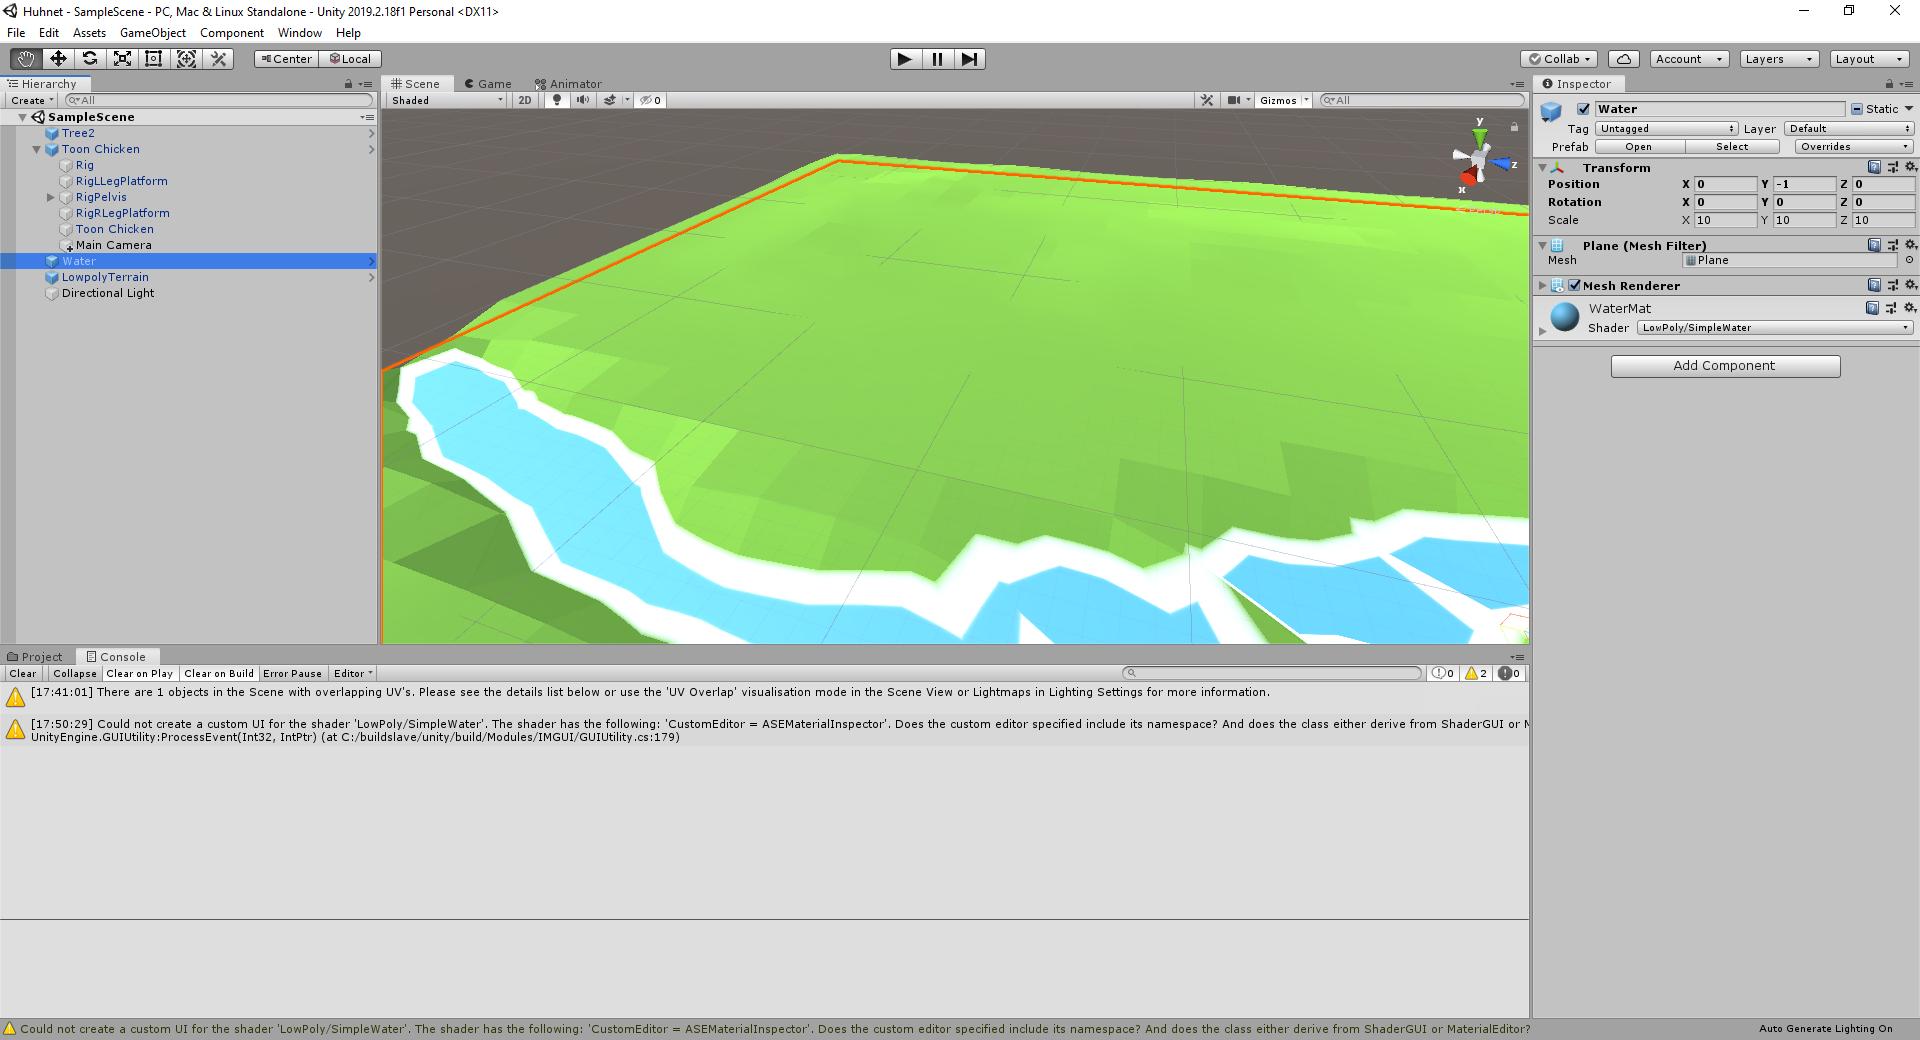
\includegraphics[scale=0.3]{img/unity1.png}
          \caption[Unity Entwicklungsumgebung.]{Unity Entwicklungsumgebung. [Quelle: Eigene Darstellung].}
          \label{fig:unity1}
        \end{figure}
        Zudem bietet Unity nicht nur eine grafische Benutzeroberfläche, 
        sondern auch viele weitere Funktionen, die im Folgenden aufgelistet werden: \\
        \begin{itemize}
          \item Grafik gemäß des aktuellen Standes der Technik
          \item Animationen, um Modelle animieren zu können
          \item Physik für das Verhalten von Objekten
          \item Musik und Geräusche, welche Stereofonie ermöglichen
          \item Selbst programmierbare Skripte, um einzelne Entitäten zu erweitern
          \item Toolkits für User Interfaces
          \item Unterstützung für Netzwerk- und Multiplayer-Anwendungen
          \item Cross-Plattform-Entwicklung, um die entwickelte Anwendung auf mehrere
          Plattformen zu veröffentlichen
        \end{itemize}
        Unity bietet eine umfangreiche Dokumentation für jede dieser Funktionalitäten.
        Entwickelt werden die sogenannten Skripts, welche dann in der Programmiersprache
        C\# zu verschiedenen Entitäten hinzugefügt werden können. Dementsprechend ist
        Erfahrung in dieser Programmiersprache notwendig, um effektiv Prototypen
        entwickeln zu können. 
        Unity stellt zusätzlich zu ihrem 3D-Editor die 
        Entwicklungsumgebung MonoDevelop zur Verfügung, mit welcher die Skripte 
        geschrieben sowie Fehlersuche und -beseitigung betrieben werden können.
        Durch die umfangreiche Benutzeroberfläche und den Funktionen benötigt Unity jedoch 
        eine lange Einarbeitungszeit. \\ \\
        Im Rahmen dieses Forschungsprojektes werden jedoch nicht alle Funktionen,
        die Unity bereitstellt, benötigt.\footnote{Unity Dokumentation | \url{https://docs.unity3d.com/Manual/} (22.11.2020).} \\
        Unity ist kostenlos nutzbar und bietet dabei den vollen Funktionsumfang\footnote{Unity Pläne | \url{https://store.unity.com/\#plans-individual} (22.11.2020).}.
      \subsubsection{Unreal Engine}
        Die Unreal Engine ist ähnlich zur 
        Unity Engine, verfolgt jedoch einige andere Ansätze. Ähnlich zur
        Unity Engine ist der weitläufige Funktionsumfang und die grafische
        Benutzeroberfläche (siehe Abb. \ref{fig:unreal1}). 
        \begin{figure}[h]
          \centering
          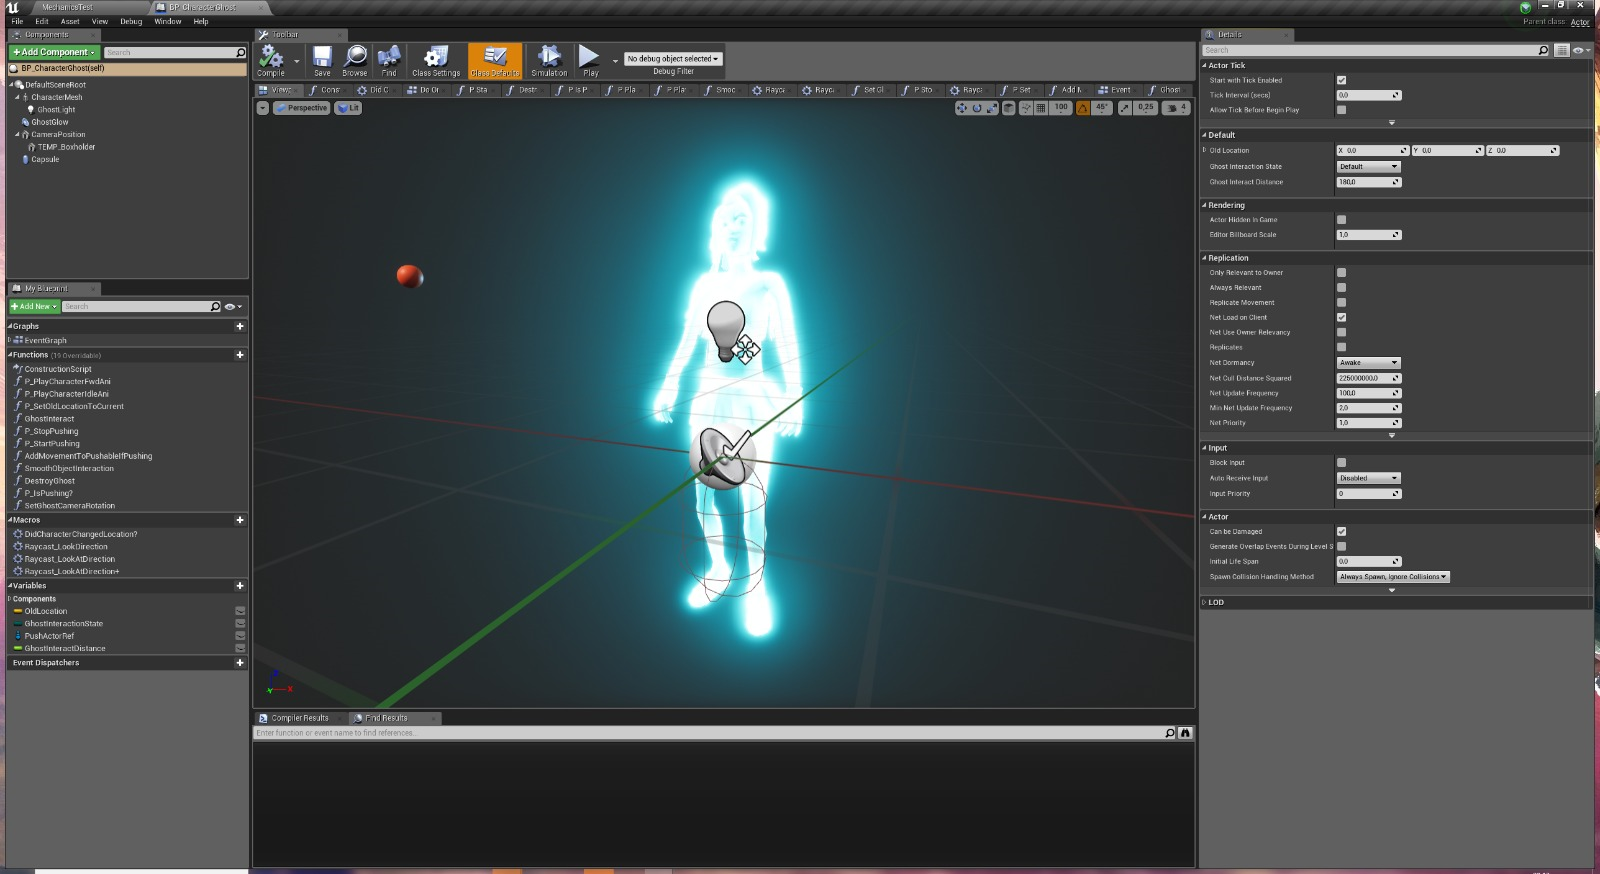
\includegraphics[scale=0.35]{img/unreal1.png}
          \caption[Unreal Engine Entwicklungsumgebung.]{Unreal Engine Entwicklungsumgebung. [Quelle: Eigene Darstellung].}
          \label{fig:unreal1}
        \end{figure}
        Auch mit Hilfe dieser Technologie lassen sich über 
        einen 3D-Editor Entitäten bearbeiten und in Szenen positionieren.
        Zusätzlich verfügt die Unreal Engine,
        für Personen die nicht programmieren können, über ein sogenanntes Blueprint-System
        (siehe Abb. \ref{fig:unreal2}).
        Damit lassen sich per Drag and Drop Algorithmen grafisch zusammenstellen. Somit
        ist Unreal Engine einsteigerfreundlich für Nicht-Entwickler.
        Komplexere Algorithmen werden in C++ entwickelt. Dementsprechend sollten 
        Kenntnisse in dieser Programmiersprache mitgebracht werden. 
        Auch dabei muss, wie bereits bei der Unity Engine aufgezeigt
        wurde, eine gewisse Einarbeitungszeit berücksichtigt werden.
        \begin{figure}[h]
          \centering
          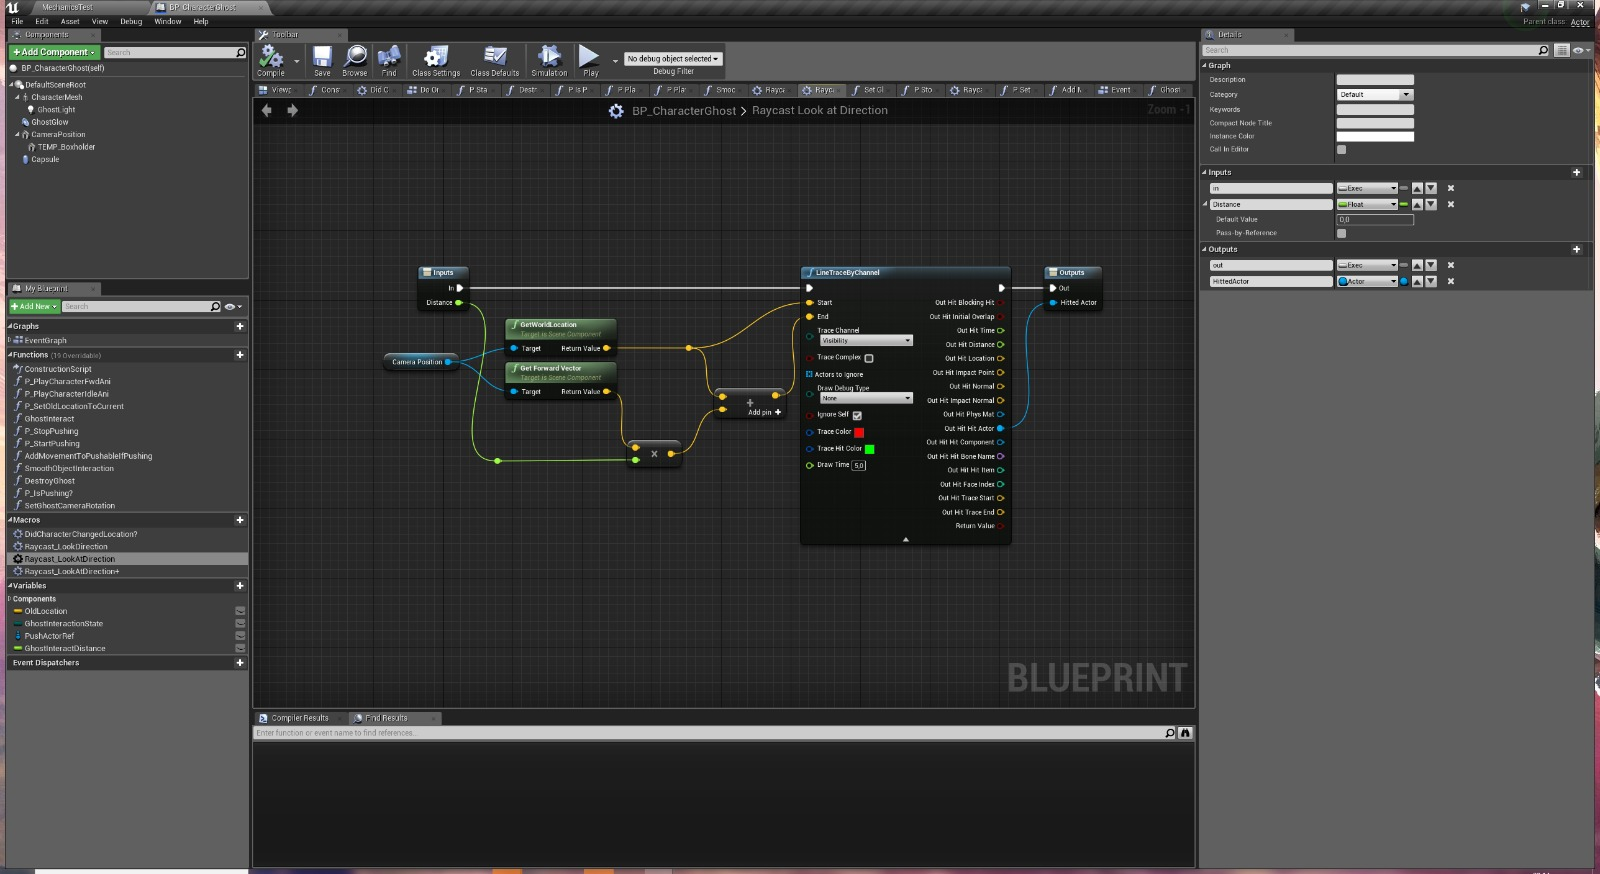
\includegraphics[scale=0.35]{img/unreal2.png}
          \caption[Unreal Engines Blueprint-System.]{Unreal Engines Blueprint-System. [Quelle: Eigene Darstellung].}
          \label{fig:unreal2}
        \end{figure} \\
        Das Endprodukt kann sowohl auf viele unterschiedliche Plattformen 
        als auch in das Web portiert werden. Die Entwicklung von Webanwendungen
        in der Unreal Engine ist jedoch nur über eine Erweiterung möglich, welche von 
        der Community entwickelt wird. Darin zeichnet sich nicht unbedingt ein Nachteil ab, 
        kann aber unter Umständen problematisch sein, denn der Support ist von der Aktivität 
        der Community abhängig, die an dieser Erweiterung arbeitet. \\
        Zum aktuellen Zeitpunkt wird die Erweiterung von der Community weiterentwickelt\footnote{Unreal Engine Dokumentation | \url{https://docs.unrealengine.com/en-US/index.html} (22.11.2020).}. \\
        Die Unreal Engine ist ebenfalls kostenlos nutzbar, sofern kein kommerzieller
        Hintergrund bei der Entwicklung einer Anwendung ist\footnote{Unreal Engine Pläne für Nicht-Spiele | \url{https://www.unrealengine.com/en-US/get-now/non-games} (22.11.2020).}.
      \subsubsection{React 360}
        React 360 ist ein Framework zur Entwicklung von Cross-Plattform-Anwendungen auf
        Basis von JavaScript. React 360 stellt eine Erweiterung von \footnote{React | \url{https://reactjs.org/} (22.11.2020).}
        für die Entwicklung von VR-Webanwendungen dar.
        Da das React-Ökosystem eine große Community mit sich bringt, gibt es viele
        Code-Pakete die zur Entwicklung von Webanwendungen mit React und React 360
        genutzt werden können.
        React 360 baut auf Three.js auf und bietet darüber hinaus ein weiteres 
        Abstraktionslevel, welches zu einer vereinfachten Entwicklung beiträgt. 
        Durch die JavaScript Syntax Extension (JSX)
        ist es möglich, einfaches HTML mit JavaScript in einer Datei zu kombinieren \footnote{JSX bei React | \url{https://reactjs.org/docs/introducing-jsx.html} (22.11.2020).}.
        Dadurch ist der Programmcode für den Entwickler lesbarer und verständlicher.
        Ein Nachteil ist, dass React 360 keinen 3D-Editor und
        keine grafische Benutzeroberfläche anbietet. 3D-Modelle, die
        an eine bestimmte Position sollen, müssen über den Programmcode positioniert und
        daraufhin kontrolliert werden. Dies bringt einen Mehraufwand mit sich. \\ \\ \\
        React 360-Anwendungen werden mit JavaScript entwickelt, wodurch ein leichter Einstieg
        ermöglicht wird. C\# und C++ können im Gegensatz zu JavaScript aufgrund der
        strengen Typsicherung als komplexe Programmiersprachen verstanden werden.
        Dieser Punkt ist für einige Entwickler ein Nachteil von JavaScript, welcher sich
        jedoch durch Hilfsmittel und die passende 
        Entwicklungsumgebung beheben lässt. \footnote{React 360 | \url{https://facebook.github.io/react-360/} (22.11.2020).} \\
        React 360 ist Open Source und steht unter der BSD-Lizenz. Demnach darf diese
        Software kostenlos verwendet, verändert und bei 
        Bedarf kommerziell vertrieben werden. Das ist einer der Gründe, weshalb
        React und React 360 eine große und aktive Community besitzen.
      \subsubsection{A-Frame}
        A-Frame ist ein Framework, mit welchem WebXR-Anwendungen
        entwickelt werden können. Dazu muss ebenfalls in der Programmiersprache 
        JavaScript entwickelt werden. A-Frame erweitert HTML um eigene 
        HTML-Elemente, welche das Benutzen von geometrischen Entitäten oder 3D-Modellen
        vereinfachen (siehe Abb. \ref{fig:aframe1}). Damit schafft A-Frame ein 
        weiteres Abstraktionslevel, wodurch das Programmieren einer VR-Webanwendung
        deklarativ wird. Prototypen lassen sich bereits ohne das Anwenden von 
        JavaScript entwickeln, sodass der Einstieg vereinfacht wird.
        \begin{figure}[h]
          \centering
          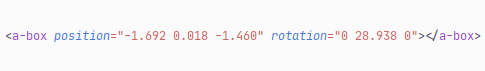
\includegraphics{img/aframe1.png}
          \caption[HTML-Element aus A-Frame.]{HTML-Element aus A-Frame. [Quelle: Eigene Darstellung].}
          \label{fig:aframe1}
        \end{figure}
        Ein weiterer Vorteil von A-Frame ist die mitgelieferte grafische 
        Benutzeroberfläche, die sich im Browser ausführen lässt 
        (siehe Abb. \ref{fig:aframe1-gui}).
        \begin{figure}[h]
          \centering
          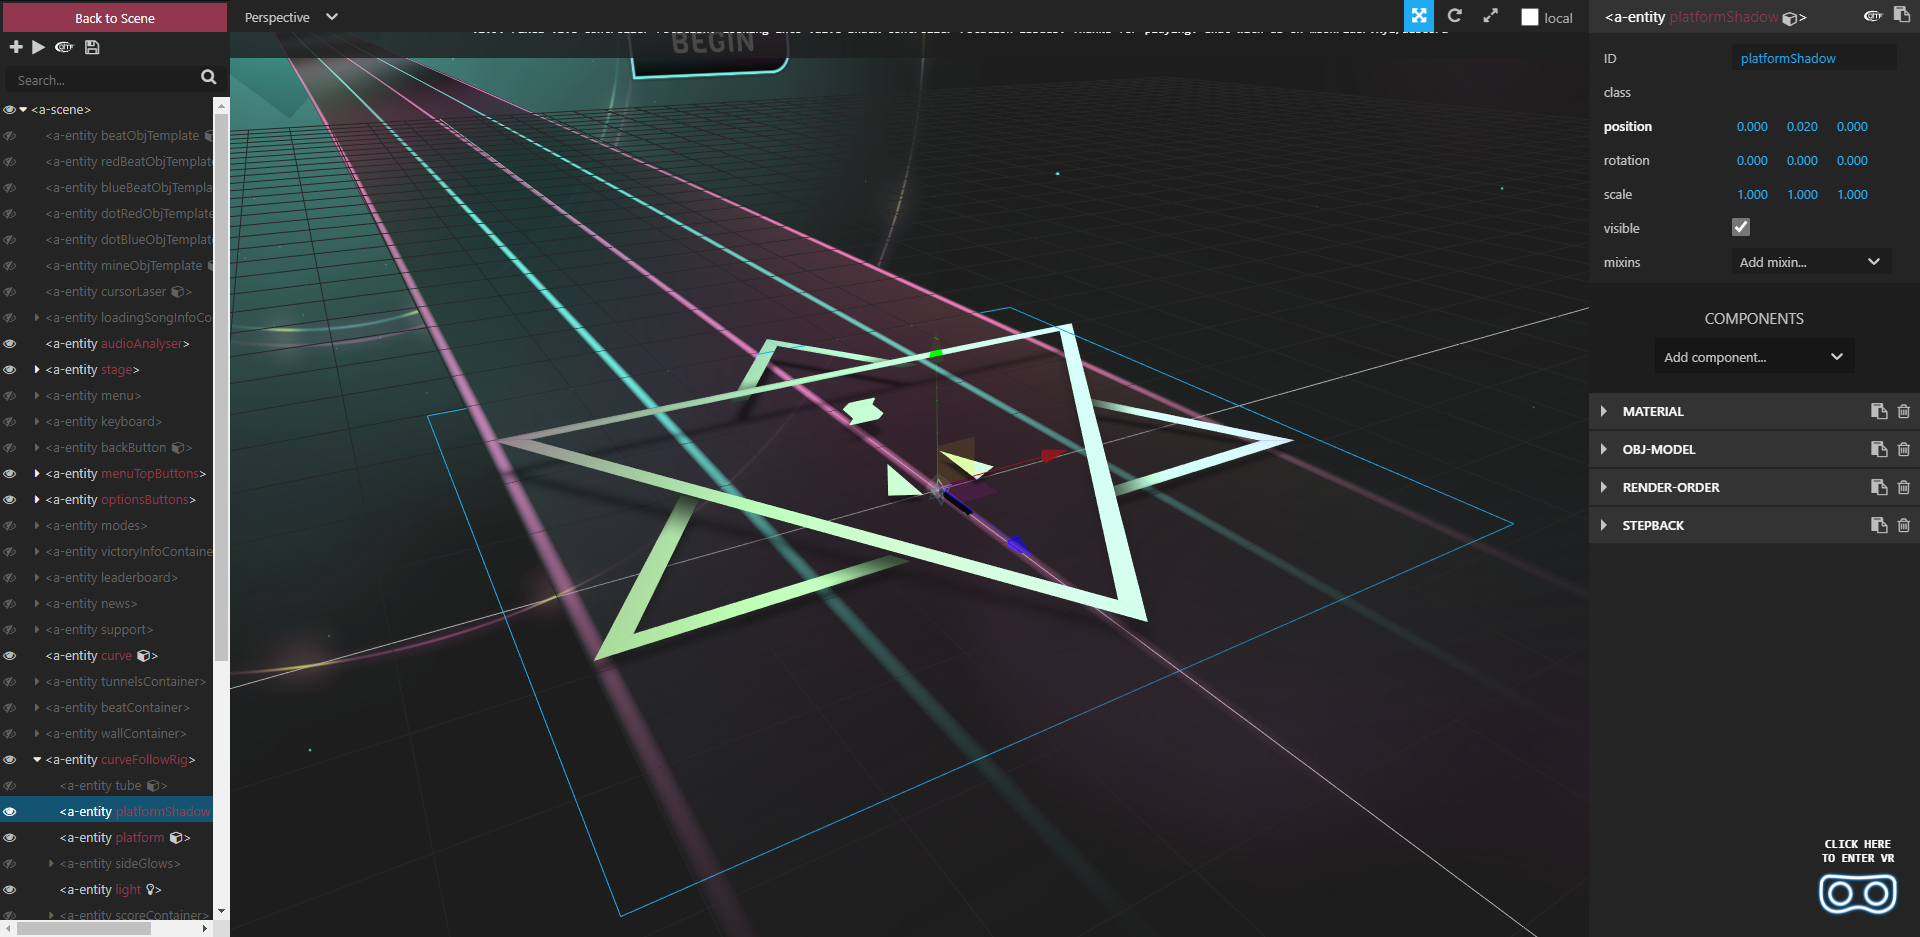
\includegraphics[scale=0.3]{img/aframe-editor.png}
          \caption[Grafische Benutzeroberfläche von A-Frame.]{Grafische Benutzeroberfläche von A-Frame. [Quelle: Eigene Darstellung].}
          \label{fig:aframe1-gui}
        \end{figure}
        Darüber lassen sich Entitäten positionieren und Komponenten zu diesen 
        hinzufügen. Wie bereits erwähnt verfügt A-Frame über eine aktive und große
        Community und bietet einen Discord-Server an\footnote{Discord ist eine Software zum Chatten und Telefonieren. Es können öffentliche Server eingerichtet werden mit verschiedenen Chat-Kanälen, in denen sich ausgetauscht werden kann. | \url{https://discord.gg/tGYjkYr} (22.11.2020).}.
        Auf diesem können jederzeit Fragen zu A-Frame gestellt werden.
        A-Frame baut auf Three.js auf und kann daher die Funktionen
        dieser Library nutzen. Bei Bedarf lässt sich über JavaScript auf 
        den vollen Funktionsumfang von Three.js innerhalb von A-Frame Komponenten
        zugreifen. Dadurch wird das Framework flexibel und mächtig. \\
        A-Frame ist Open Source und steht unter der MIT-Lizenz. Somit kann dieses
        Framework kostenlos und ohne Einschränkungen zur Entwicklung der 
        Prototypen verwendet werden. \\ \\
      \subsubsection{Three.js}
        Three.js ist eine Library die auf JavaScript basiert und demnach auch
        für diese Programmiersprache vorgesehen ist. Ähnlich wie A-Frame bietet
        Three.js eine Anlaufstelle für ihre Community, die über einen Discord-Server
        und ein Forum diskutieren kann. Auf der Webseite lassen sich einige 
        Beispielprojekte finden die Three.js nutzen. Darunter finden sich auch
        A-Frame und React 360. \\
        Three.js bietet wie Unity und Unreal Engine vorprogrammierte Funktionen
        wie Physik, Animationen oder einen 3D-Editor an. Der Editor ist, anders
        als bei A-Frame, nicht im eigenen Projekt integriert, sondern über die
        Webseite von Three.js erreichbar. In diesem Editor können die
        Funktionen anhand einer grafischen Benutzeroberfläche ausprobiert werden. \\
        Auf der Webseite wird eine eigene Tutorialreihe angeboten, in der
        auf die Entwicklung von WebVR-Anwendungen eingegangen wird. \\
        Da keine grafische Benutzeroberfläche mitgeliefert wird und alles über den
        Programmcode erstellt werden muss, steigt die Komplexität dieser
        Technologie. \\
        Three.js ist Open Source, steht unter der MIT-Lizenz und lässt sich daher
        kostenfrei ohne Einschränkungen für die Entwicklung der Prototypen nutzen.\footnote{Three.js Webseite | \url{https://threejs.org/} (22.11.2020).}
      \subsubsection{Auswahl der Technologie}
        Nachfolgend lassen sich in Tabelle \ref{tab:funktionsumfang-technologien} 
        die Vor- und Nachteile der zuvor vorgestellten Technologien festhalten.
        \begin{table}[h]
          \begin{center}
            \begin{tabular}{| c | c | c | c | c | c | c |}
              \hline
              & \textbf{Unity} & \textbf{Unreal Engine} & \textbf{React 360} & \textbf{A-Frame} & \textbf{Three.js} \\ \hline
              \textbf{GUI} & \checkmark & \checkmark & X & \checkmark & X \\ \hline
              \textbf{3D-Editor} & \checkmark & \checkmark & X & \checkmark &  \checkmark \\ \hline
              \textbf{Einsteigerfreundlich} & X & X & \checkmark & \checkmark & \checkmark \\ \hline
              \textbf{Große Community} & \checkmark & \checkmark & \checkmark & \checkmark & \checkmark \\ \hline
              \textbf{Open Source} & X & X & \checkmark & \checkmark & \checkmark \\ \hline
              \textbf{Kostenlos nutzbar} & \checkmark & \checkmark & \checkmark & \checkmark & \checkmark \\ \hline
            \end{tabular}
            \caption[Funktionsumfang aller Technologien.]{Funktionsumfang aller Technologien. [Quelle: Eigene Darstellung].\label{tab:funktionsumfang-technologien}}
          \end{center}
        \end{table}
        Wie dieser Tabelle zu entnehmen, weisen die meisten Vorteile
        die Technologien A-Frame und Three.js auf.
        Da in diesem Forschungsprojekt bereits Kentnisse im Bereich
        JavaScript und Webentwicklung vorliegen, ist die Entwicklung 
        mit Hilfe einer der beiden Technologien möglich. \\
        A-Frame bietet zusätzlich zu Three.js eine grafische Oberfläche, welche
        in jedem Projekt automatisch integriert und über den Browser zu
        bedienen ist. Der volle Funktionsumfang von Three.js ist 
        auch weiterhin in A-Frame
        enthalten, da das Framework auf dieser Library aufbaut. 
        Die A-Frame Technologie, welche ein weiteres Abstraktionslevel sowie
        vorgefertigte Funktionen aufweist, die in Three.js selbstständig
        implementiert werden müssten, benötigt zusätzlich keine 
        große Einarbeitungszeit. Diese Gründe sprechen zusammengefasst 
        für einen sinnvollen 
        Einsatz der Technologie im Rahmen dieses Projekts. \\
      \subsubsection{Weitere Hilfsmittel}
        Zusätzlich zur Wahl der Technologie lassen sich weitere Hilfsmittel
        in die Entwicklung der Prototypen hinzuziehen. Diese sollen das
        Entwickeln und Verwalten des Codes und der Dateien vereinfachen und
        Optimierungen zur Peformanz der Anwendung mit sich
        bringen. \\
        Für die Versionsverwaltung wird \textbf{Git}\footnote{Git | \url{https://git-scm.com/} (22.11.2020).} in Kombination mit GitHub
        verwendet. Dadurch können Funktionen implementiert werden ohne den
        aktuellen und lauffähigen Code zu beeinflussen. Bei erfolgreichen
        Tests der neuen Funktionen kann dieser Code in die aktuelle Version
        hinzugefügt werden. Bei Bedarf kann auf den alten Code zugegriffen 
        und die Anwendung auf diesen Stand zurückgebracht werden. \\
        Für eine verbesserte Typsicherheit in JavaScript und produktiveres
        Programmieren wird \textbf{TypeScript}\footnote{TypeScript | \url{https://www.typescriptlang.org/} (22.11.2020).} verwendet. So finden Konstrukte
        wie Interfaces aus der objektorientierten Programmierung auch
        Anwendung in JavaScript. Dies vereinfacht 
        die Entwicklung mit JavaScript und gestaltet die Anwendung skalierbarer. \\
        Das letzte Hilfsmittel ist \textbf{Webpack}\footnote{Webpack | \url{https://webpack.js.org/} (22.11.2020).}. Dies
        hilft bei der Optimierung des Codes, da es den gesamten JavaScript-Code
        in eine Datei zusammenfügt und diese keine Leerzeichen, Tabulatoren
        oder Umbrüche beinhaltet. Dadurch ist die Größe der Datei minimiert.
    \subsection{Entwicklung der Prototypen}
      Zu Beginn wurde durch die Auseinandersetzung mit dem Framework ein 
      Bereich zum Entwickeln geschaffen, in dem verschiedene 
      Ansätze zum Darstellen von
      Gemälden und Archivalien in einer virtuellen Welt ausprobiert werden
      können. \\
      Entwickelt wird in der Entwicklungsumgebung WebStorm von Jetbrains\footnote{WebStorm | \url{https://www.jetbrains.com/de-de/webstorm/} (22.11.2020).}.
      Die VR-Brille, mit der die Anwendungen getestet werden, ist die Oculus Quest,
      welche von der Technischen Hochschule Köln gestellt wird. Diese verwendet
      den Browser Firefox Reality, welcher viele Funktionen für Entwickler 
      bietet \footnote{Firefox Reality | \url{https://mixedreality.mozilla.org/firefox-reality} (22.11.2020).}. \\
      Zunächst soll ein technischer Prototyp entwickelt werden, welcher das
      Fortbewegen in der virtuellen Welt durch das Angucken von Objekten ermöglicht.
      Auch sollen Gemälde und deren Beschreibung angezeigt werden können. Sobald
      die ersten technischen Anforderungen erfüllt sind, 
      sollen weitere Prototypen entwickelt werden.
      \subsubsection{Technischer Prototyp}
        Der erste technische Prototyp zeigt, wie eine blickorientierte
        Steuerung und die Gemälde von Cranach mit Hilfe von A-Frame 
        entwickelt werden können. Zusätzlich bildet dieser das Fundament 
        für die weiteren Prototypen. \\
        Um den ersten Prototypen zu entwickeln, musste vorerst das Prinzip
        von A-Frame, im Hinblick auf die Darstellung von Inhalten mittels HTML
        und JavaScript, verstanden werden. \\
        Bevor mit der Entwicklung eines Prototypen mit JavaScript begonnen
        werden konnte, musste grundlegend ein Gemälde von Cranach innerhalb
        einer virtuellen Welt dargestellt werden. Dafür wurde eine statische
        \texttt{index.html}-Datei benötigt, welche die aktuelle stabile 
        Version von A-Frame importiert (siehe Abb. \ref{fig:index1}).
        \begin{figure}
          \centering
          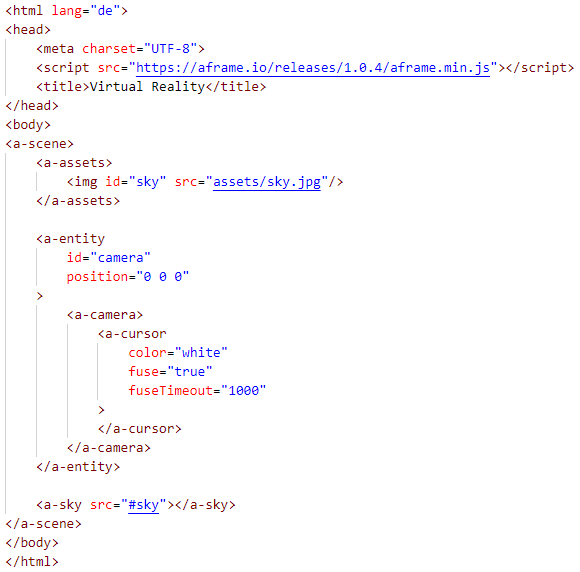
\includegraphics[scale=0.9]{img/coding/index1.png}
          \caption[Erste Version einer \texttt{index.html}-Datei.]{Erste Version einer \texttt{index.html}-Datei. [Quelle: Eigene Darstellung].}
          \label{fig:index1}
        \end{figure}
        Neben den notwendigen HTML-Tags, die für eine valide HTML-Datei
        notwendig sind, kamen \texttt{<a-scene>}, \texttt{<a-assets>},
        \texttt{<a-entity>}, \texttt{<a-camera>}, \texttt{<a-cursor>}
        und \texttt{<a-sky>} hinzu. A-Frame-HTML-Tags lassen sich durch
        das Präfix \texttt{a-} erkennen. \\
        \texttt{\textbf{<a-scene>}} ist immer das erste und notwendige
        HTML-Tag einer A-Frame-Anwendung. Durch dieses Tag erkennt das Framework, 
        dass es sich hierbei um eine A-Frame-Szene handelt. 
        So müssen alle weiteren HTML-Tags, welche im Rahmen von A-Frame
        entwickelt werden, innerhalb dieses Tags platziert werden. \\
        \texttt{\textbf{<a-assets>}} beinhaltet alle notwendigen Assets für die 
        VR-Anwendung. Darin können 3D-Modelle oder 
        Bilder (Texturen, Icons, etc.) eingefügt werden. 
        Sofern möglich, empfiehlt A-Frame alle benötigten Assets in \texttt{<a-assets>}
        hinzuzufügen, da diese im Cache gespeichert werden und ein Neuladen
        der Anwendung beschleunigen. \\ \\
        Bei \texttt{\textbf{<a-entity>}} handelt es sich um eine einfache Entität,
        welche vorerst keine Darstellung innerhalb der VR-Anwendung haben
        muss. Oft kann dieses Tag auch als Wrapper für mehrere Tags verwendet
        werden. 
        Dies hat den Vorteil, dass nur jene Entität angesprochen werden muss,
        um alle Entitäten innerhalb dieser bewegen zu können.
        Das innerhalb des \texttt{<a-entity>}-Tags auftretende Attribut
        \texttt{id} besitzt keine A-Frame-spezifische Definition und weist
        somit die selbe Funktion eines normalen \texttt{id}-Attributs auf. \\
        Das Attribut \texttt{position} hingegen gibt die Position als 3D Vektor, 
        relativ zum Nullpunkt der Weltkoordinaten, an. Die Entität des
        Beispiels in Abbildung \ref{fig:index1} befindet
        sich demnach genau auf dem Nullpunkt der Weltkoordinaten. \\
        Das HTML-Tag \texttt{\textbf{<a-camera>}} stellt die Kamera und
        somit die Augen des Benutzers innerhalb der VR-Anwendung dar.
        Demnach ist die Position der Kamera dieselbe wie die 
        des Benutzers. 
        Durch das Fehlen einer Kamera kann keine virtuelle Welt gesehen werden,
        wodurch dieser HTML-Tag zwingend notwendig ist. \\
        Innerhalb der \texttt{<a-camera>}-Entität befindet sich 
        \texttt{\textbf{<a-cursor>}}. Mit diesem Cursor kann der Benutzer
        auf bestimmte Entitäten innerhalb einer virtuellen Welt zeigen. Durch
        die Attribute \texttt{fuse} und \texttt{fuseTimeout} lassen sich 
        zusätzlich Entitäten anklicken. A-Frame bietet somit grundlegend 
        eine Implementation für die blickorientierte Steuerung. Durch 
        \texttt{fuse=true} wird diese aktiviert.
        \texttt{fuseTimeout="1000"} gibt an, wie viel Millisekunden 
        auf eine Entität geschaut werden muss, 
        damit bei dieser der EventListener des Typs
        \texttt{click} ausgelöst wird. 
        Für die Reaktion einer Entität auf einen Klick, muss 
        ein EventListener für \texttt{click} innerhalb dieser festgelegt
        werden. \\
        Das Attribut \texttt{color} legt die Farbe des Cursors fest. \\
        Das HTML-Tag \texttt{\textbf{<a-sky>}} bietet eine fertige Lösung,
        um einen Himmel innerhalb der virtuellen Welt anhand einer Bilddatei
        anzuzeigen. Durch das Attribut \texttt{src="\#sky"} wird die
        Bilddatei mit der ID \texttt{\#sky} aus den Assets geladen. Diese
        Schreibweise ersetzt letztlich die Angabe eines Pfades. \\
        Unter Anwendung dieser vorgestellten Schritte ergibt sich für
        die \texttt{index.html} die in Abbildung \ref{fig:vr-welt1} gezeigte
        erste virtuelle Welt.
        \begin{figure}
          \centering
          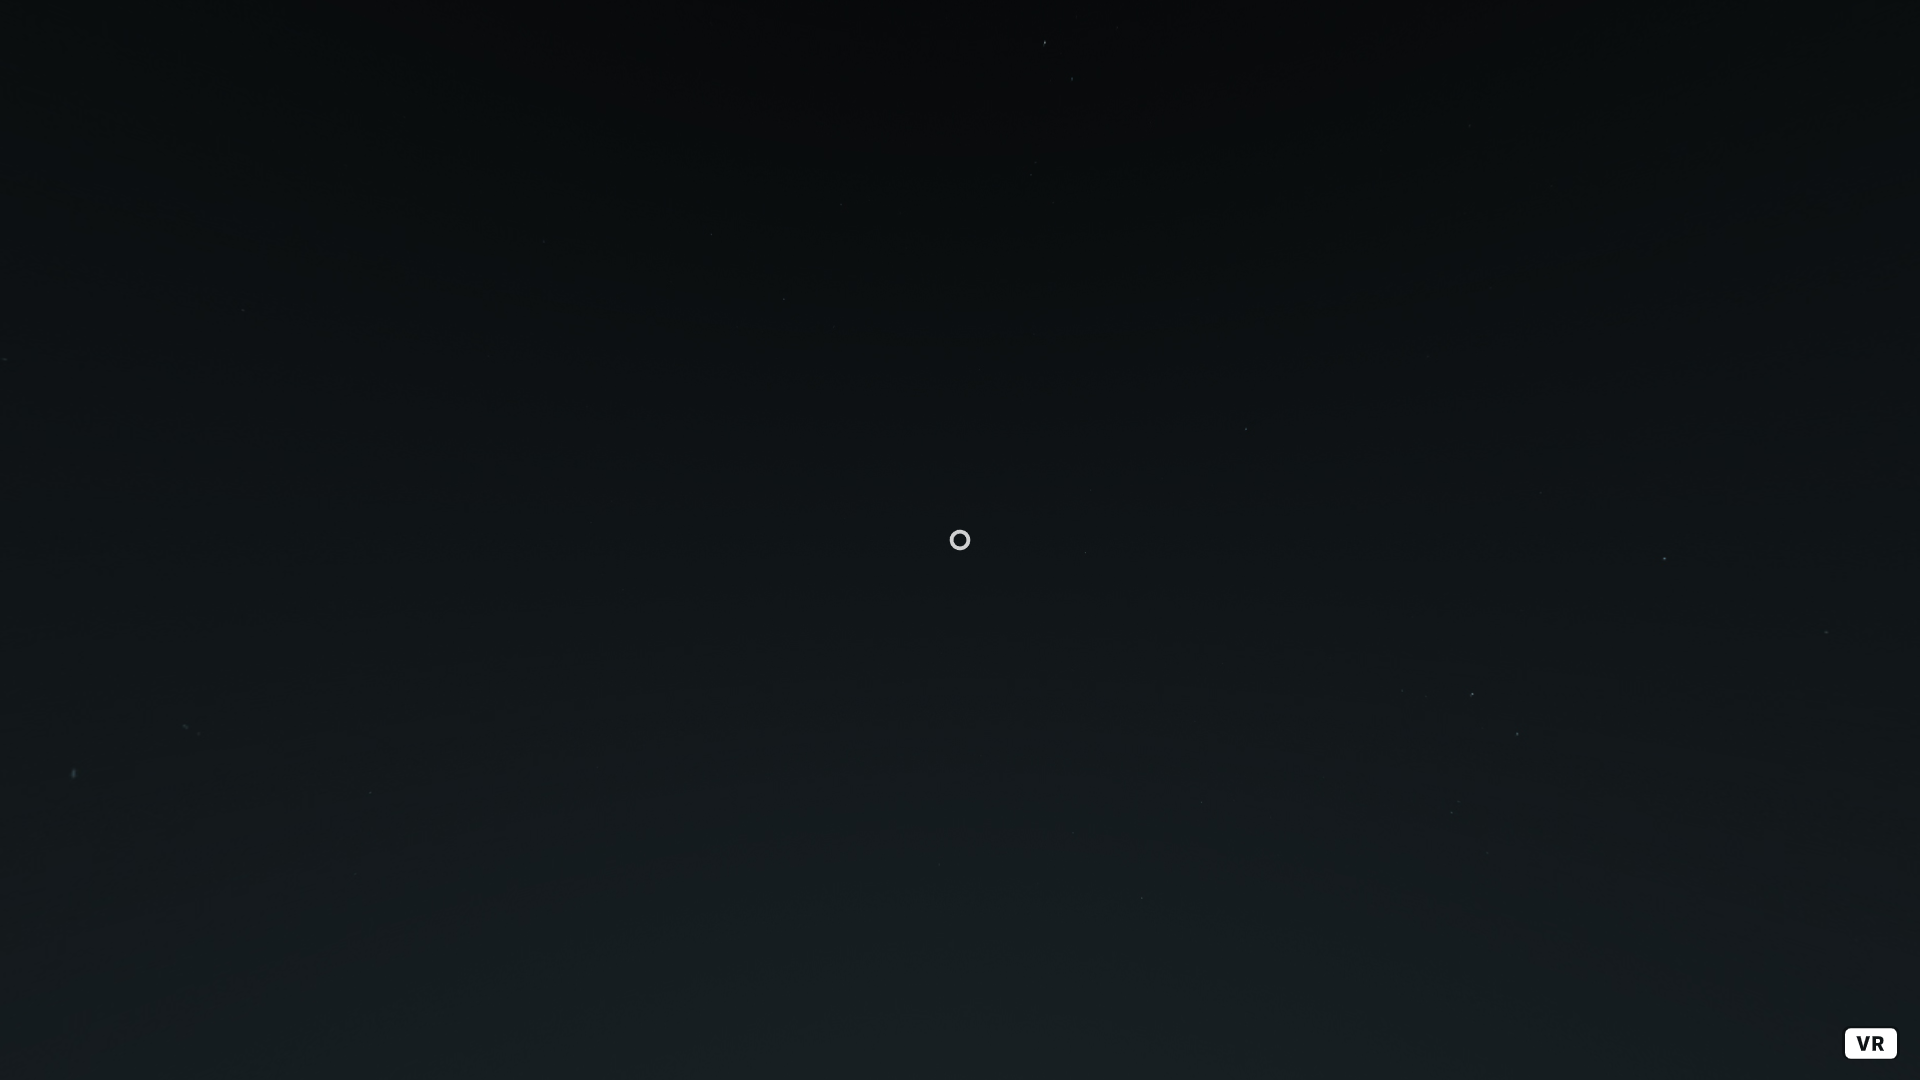
\includegraphics[scale=0.3]{img/coding/vr-welt1.png}
          \caption[Erste virtuelle Welt.]{Erste virtuelle Welt. [Quelle: Eigene Darstellung].}
          \label{fig:vr-welt1}
        \end{figure}
        Der Cursor der Anwendung befindet sich in der Mitte und ist als weißer
        Kreis dargestellt. Unten rechts befindet sich der VR-Button, welcher
        immer von A-Frame mitgerendert wird. Ein Klick auf diesen Button 
        aktiviert den VR-Modus der Webanwendung. \\
        Als nächster Schritt soll ein Gemälde angezeigt werden. In diesem
        Beispiel wird das Gemälde aus dem Cranach Digital Archive
        mit der ID \texttt{DE\_MdbKL\_946} verwendet. A-Frame stellt
        den HTML-Tag \texttt{\textbf{<a-image>}} für die Anzeige von Bildern
        zur Verfügung.
        Das Seitenverhältnis der Bilder wird dabei nicht beibehalten, wodurch
        dieses durch die Attribute \texttt{width} und \texttt{height} 
        festgelegt werden muss. Dieser Image-Tag wird innerhalb der
        \texttt{<a-scene>} in Meterangaben platziert (siehe Abb. \ref{fig:a-image1}).
        An dieser Stelle bietet A-Frame die Möglichkeit, häufig benutzte
        Eigenschaften von Three.js, wie \texttt{height}, \texttt{width}
        oder \texttt{color}, über HTML-Attribute festzulegen. Durch diese
        Abstraktion muss nicht über JavaScript die Entität manipuliert
        werden. Das vereinfacht den Prozess des Prototypings.
        \begin{figure}
          \centering
          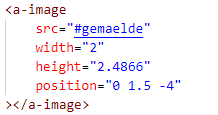
\includegraphics{img/coding/a-image1.png}
          \caption[Image-Tag von A-Frame für das Einbinden von Bildern.]{Image-Tag von A-Frame für das Einbinden von Bildern. [Quelle: Eigene Darstellung].}
          \label{fig:a-image1}
        \end{figure}
        Die Verschiebung einer Entität ist immer 
        von ihrem eigenen Mittelpunkt ausgehend. 
        Das Resultat dieser Arbeitsschritte wird in Abbildung \ref{fig:vr-welt2}
        verdeutlicht.
        \begin{figure}[h]
          \centering
          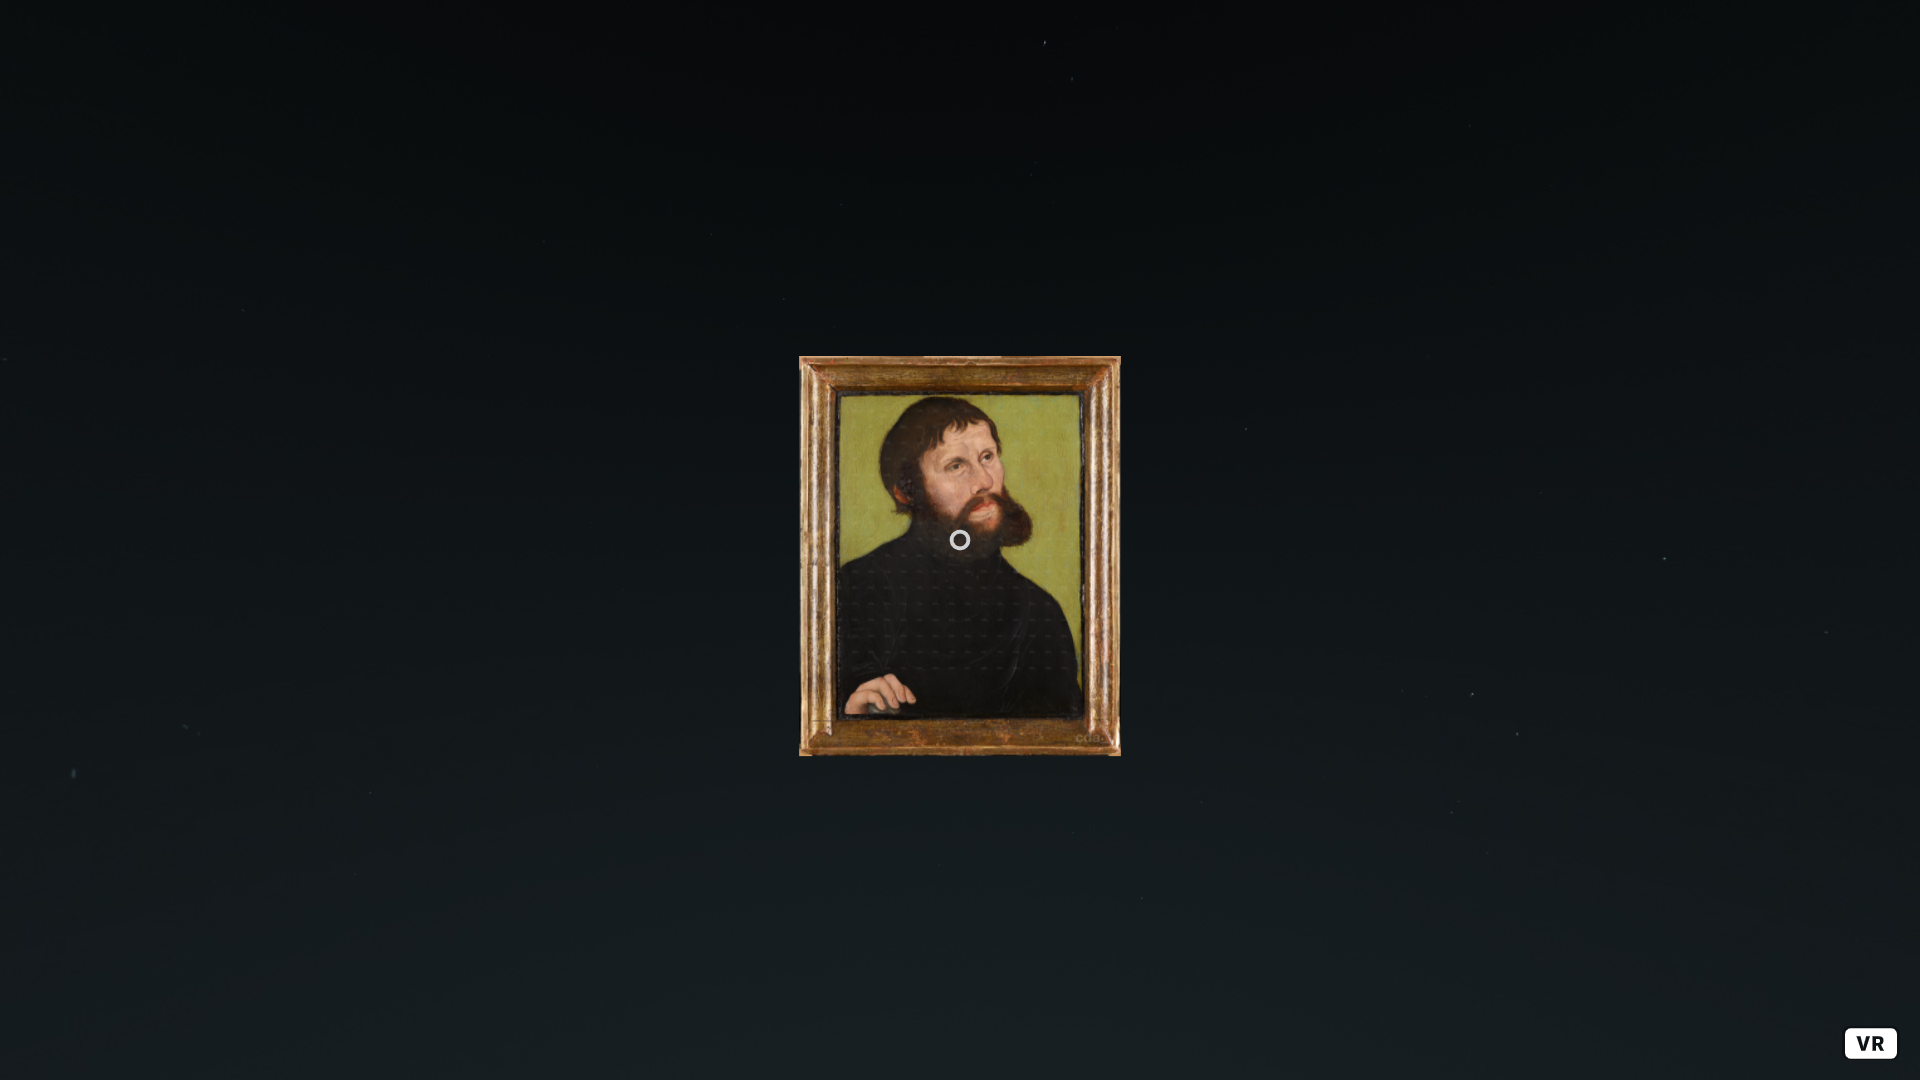
\includegraphics[scale=0.3]{img/coding/vr-welt2.png}
          \caption[Gemälde innerhalb der virtuellen Welt.]{Gemälde innerhalb der virtuellen Welt. [Quelle: Eigene Darstellung].}
          \label{fig:vr-welt2}
        \end{figure} \\
        In weiteren Schritten wurde eine Steuerung durch das Anschauen von Entitäten
        entwickelt. Da A-Frame bereits eine Implementation für das 
        blickorientierte Klicken zur Verfügung stellt, musste eine
        Entität erzeugt werden, welche auf Klicken reagiert. Das Framework
        bietet zwei Möglichkeiten EventListener zu registrieren. Die Erste
        besteht darin, die EventListener ebenfalls in HTML
        als Attribut festzulegen. In Abbildung \ref{fig:a-image2} wird
        ein \texttt{click}-EventListener registriert, welcher die Komponente 
        über \texttt{visible=true} sichtbar macht. Die zweite Möglichtkeit
        umfasst das Registrieren eines EventListeners über JavaScript. Diese
        erlaubt den Zugriff auf Three.js innerhalb einer Entität.
        \begin{figure}[h]
          \centering
          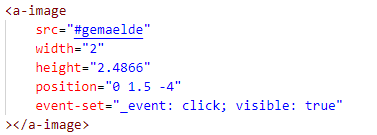
\includegraphics{img/coding/a-image2.png}
          \caption[Event Registrierung innerhalb von HTML.]{Event Registrierung innerhalb von HTML. [Quelle: Eigene Darstellung].}
          \label{fig:a-image2}
        \end{figure}
        Um einen EventListener mit JavaScript umzusetzen, musste eine Komponente
        entwickelt werden. Komponenten in A-Frame sind wiederverwendbare
        Code-Module, welche zu beliebigen Entitäten hinzugefügt werden
        können. Diese Entitäten übernehmen die Funktionen jener Komponente.
        Der Aufbau einer solchen Komponente ist in Abbildung \ref{fig:komponente1}
        dargestellt.
        \begin{figure}[h]
          \centering
          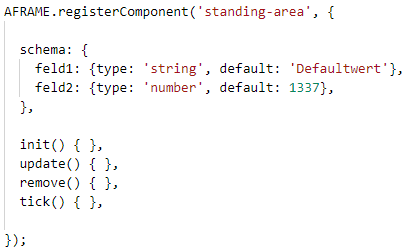
\includegraphics{img/coding/komponente1.png}
          \caption[Aufbau einer Komponente in A-Frame.]{Aufbau einer Komponente in A-Frame. [Quelle: Eigene Darstellung].}
          \label{fig:komponente1}
        \end{figure} \\
        Mit \texttt{AFRAME.registerComponent(...)} wird eine
        Komponente für A-Frame erstellt. \\
        Das erste Argument ist vom Typ \texttt{string}
        und beinhaltet den Namen der jeweiligen Komponente. Das zweite Argument
        ist ein Objekt, welches die Lifecycle-Methoden sowie ein Schema 
        einer A-Frame Komponente enthält.
        Das Feld \texttt{\textbf{schema}} gibt an, welche Werte
        innerhalb des HTML über das Attribut \texttt{standing-area} 
        in die Komponente hineingeben werden können. \texttt{feld1}
        und \texttt{feld2} sind die Namen dieser Eigenschaften. Mit \texttt{type}
        lässt sich der Typ für den Wert festlegen. \texttt{default}
        gibt einen Standardwert zurück, sofern keine Information zu dieser
        Eigenschaft mitgegeben wurde. In Abbildung \ref{fig:komponente2} müsste
        demnach das Attribut um \texttt{standing-area="feld1: Test; feld2: 1338"}
        erweitert werden, damit der Standardwert überschrieben und ein
        neuer hineingegeben werden kann. Die Werte in \texttt{schema} können
        über \texttt{this.data.feld1} oder \texttt{this.data.feld2} 
        innerhalb der Komponente aufgerufen werden. \\
        Die \texttt{\textbf{init}}-Methode wird beim ersten Laden einer
        Entität mit einer Komponente ausgeführt. Dabei werden
        initiale Werte festgelegt. \\ \\
        Die \texttt{\textbf{update}}-Methode wird zunächst nach der
        \texttt{init}-Methode sowie bei jeder Veränderung der
        Attribute der Entität ausgeführt. \\
        Sofern die Entität und ihre Komponente gelöscht wird, wird einmalig
        die \texttt{\textbf{remove}}-Methode ausgeführt. \\
        Die \texttt{\textbf{tick}}-Methode ist abhängig von der Bildrate der
        Anwendung. Beträgt die FPS (Bilder pro
        Sekunde) der Anwendung 60, dann wird diese Methode 60-Mal ausgeführt. \\
        Um auf A-Frame Funktionen innerhalb der TypeScript-Datei zugreifen
        zu können, wurde A-Frame zunächst mit einem Packetmanager wie yarn\footnote{yarn | \url{https://yarnpkg.com/} (22.11.2020).}
        oder npm\footnote{npm | \url{https://www.npmjs.com/} (22.11.2020).} installiert. 
        Aufgrund dessen konnte die Importierung
        von A-Frame innerhalb der HTML-Datei entfernt werden, da
        lediglich die \texttt{bundle.js}, welche von Webpack generiert wird,
        importiert werden muss. Diese beinhaltet den gesamten Code, so auch den
        der importierten Module innerhalb einer Komponente. \\
        Die in Abbildung \ref{fig:komponente1} gezeigte Komponente ließ
        sich über HTML einer Entität hinzufügen (siehe Abb. \ref{fig:komponente2}).
        \begin{figure}[h]
          \centering
          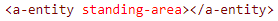
\includegraphics{img/coding/komponente2.png}
          \caption[A-Frame Entität mit hinzugefügter Komponente.]{A-Frame Entität mit hinzugefügter Komponente. [Quelle: Eigene Darstellung].}
          \label{fig:komponente2}
        \end{figure} \\
        Um das Teleportieren eines Benutzers auf die Position der Entität, 
        welche angeguckt wird, umzusetzen, wurde eine \texttt{<a-box>}
        verwendet. Diese erhält die Komponente \texttt{standing-area},
        wie Abbildung \ref{fig:standing-area1} zeigt.
        \begin{figure}[h]
          \centering
          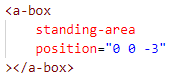
\includegraphics{img/coding/standing-area1.png}
          \caption[a-box mit der Komponente \texttt{standing-area}.]{a-box mit der Komponente \texttt{standing-area}. [Quelle: Eigene Darstellung].}
          \label{fig:standing-area1}
        \end{figure} \\
        Abbildung \ref{fig:standing-area2} stellt den zugehörigen Code
        innerhalb der Komponente \texttt{standing-area} dar.
        \begin{figure}
          \centering
          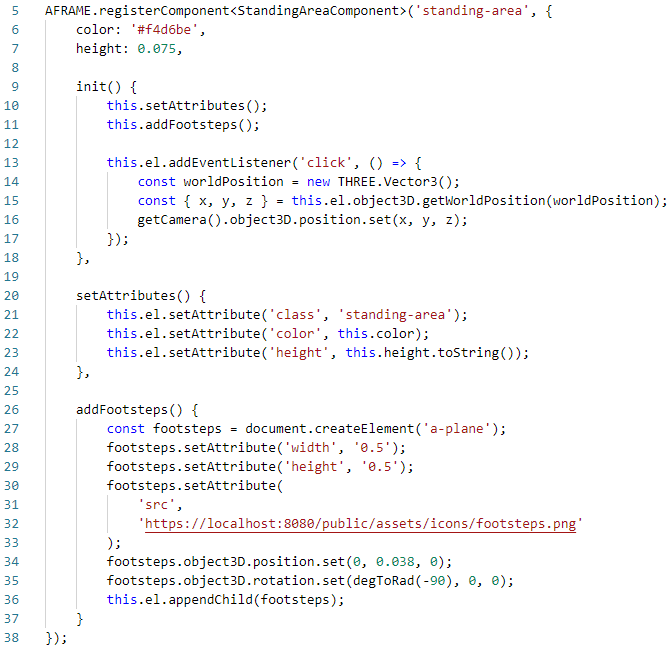
\includegraphics[scale=0.9]{img/coding/standing-area2.png}
          \caption[TypeScript-Code der Komponente \texttt{standing-area}.]{TypeScript-Code der Komponente \texttt{standing-area}. [Quelle: Eigene Darstellung].}
          \label{fig:standing-area2}
        \end{figure}
        In dieser Abbildung zeigen sich einige von A-Frame gestellten
        Vereinfachungen. Zur Veränderung der Oberflächentextur
        einer Entität wurde das HTML-Attribut \texttt{src} angewendet
        (siehe Abb. \ref{fig:standing-area2}, Zeile 30-33). 
        Diese Schreibweise erinnert an das klassische
        HTML-Attribut von einem \texttt{img}-Tag.
        HTML-Attribute, wie \texttt{width},
        \texttt{height} oder \texttt{src} wurden ebenfalls über den Code
        festgelegt 
        (siehe Abb. \ref{fig:standing-area2}, Zeile 28-33). \\
        A-Frame-Tags lassen sich über JavaScript wie normale HTML-Tags
        generieren und beispielsweise mit der Methode \texttt{querySelector}
        selektieren
        (siehe Abb. \ref{fig:standing-area2}, Zeile 27). Über \texttt{this.el}
        lässt sich auf die Entität der Komponente zugreifen. \\
        \texttt{color} und \texttt{height} 
        (siehe Abb. \ref{fig:standing-area2}, Zeile 6-7)
        sind zwei selbst festgelegte
        Eigenschaften, welche nicht zwingend in einer generellen
        A-Frame Komponente
        vorhanden sein müssen. Selbst festgelegte Eigenschaften können
        auch genutzt werden, um den state (Zustand) einer Komponente
        zu speichern. \texttt{color} gibt die Farbe der \texttt{<a-box>}
        an und \texttt{height} die Höhe dieser. \\
        Die Komponente \texttt{standing-area} führt in ihrer \texttt{init}-
        Methode zunächst die beiden internen Methoden \texttt{setAttributes}
        und \texttt{addFootsteps} aus (siehe Abb. \ref{fig:standing-area2}, Zeile 10-11).
        Erstere fügt die notwendigen
        Attribute hinzu, um das Erscheingungsbild der Entität in der
        virtuellen Welt festzulegen. \texttt{class} ist dabei nicht
        zwingend notwendig, erleichtert jedoch zukünftig das selektieren
        dieser Entität. Die zweite Methode erzeugt das Element 
        \texttt{<a-plane>}, bei welchem es sich um eine zweidimensionale
        Fläche handelt
        (siehe Abb. \ref{fig:standing-area2}, Zeile 27). 
        Durch das Attribut \texttt{src} erhält diese Fußabdrücke
        als Textur (siehe Abb. \ref{fig:standing-area2}, Zeile 30-33).
        A-Frame empfiehlt in den Best Practices\footnote{A-Frame Best Practices | \url{https://aframe.io/docs/1.0.0/introduction/best-practices.html} (22.11.2020).}
        die Eigenschaften
        \texttt{position} und \texttt{rotation} über die Schnittstelle
        von Three.js zu manipulieren (siehe Abb. \ref{fig:standing-area2}, Zeile 34-35). \\
        Dieses Verfahren ist verhältnismäßig schneller zu berechnen 
        und spart gleichzeitig Leistung ein. \\
        Das \texttt{<a-plane>}-Tag wird über die \texttt{<a-box>}
        positioniert. Dadurch befindet sich dieses Element 
        innerhalb des \texttt{<a-box>}-Tags im DOM (siehe Abb. \ref{fig:standing-area2}, Zeile 36).
        Befinden sich Entitäten innerhalb Anderer,
        werden deren Positionsangaben relativ zum Mutterelement angegeben
        (siehe Abb \ref{fig:standing-area2}, Zeile 34). \\
        Zuletzt wurde in der \texttt{init}-Methode der \texttt{click}-EventListener
        hinzugefügt (siehe Abb. \ref{fig:standing-area2}, Zeile 13-17).
        Durch den Aufruf von \texttt{.object3D} eines HTML-Elements kann
        auf die Object3D Repräsentation von Three.js zugegriffen werden.
        Bei einem Klick auf die Entität wird die aktuelle Weltposition
        ausgelesen und der Kamera hinzugefügt 
        (siehe Abb. \ref{fig:standing-area2}, Zeile 15-16). \\
        Die 
        \texttt{getCamera}-Methode ist eine globale Methode, 
        welche das Kamera-Element zurückliefert. 
        Das Ergebnis des vorgestellten Codes umfasst die Teleportation
        des Benutzers zur jeweiligen Standfläche, nachdem er diese 1 Sekunde
        angeschaut hat
        (siehe Abb. \ref{fig:standing-area3}).
        \begin{figure}[h]
          \centering
          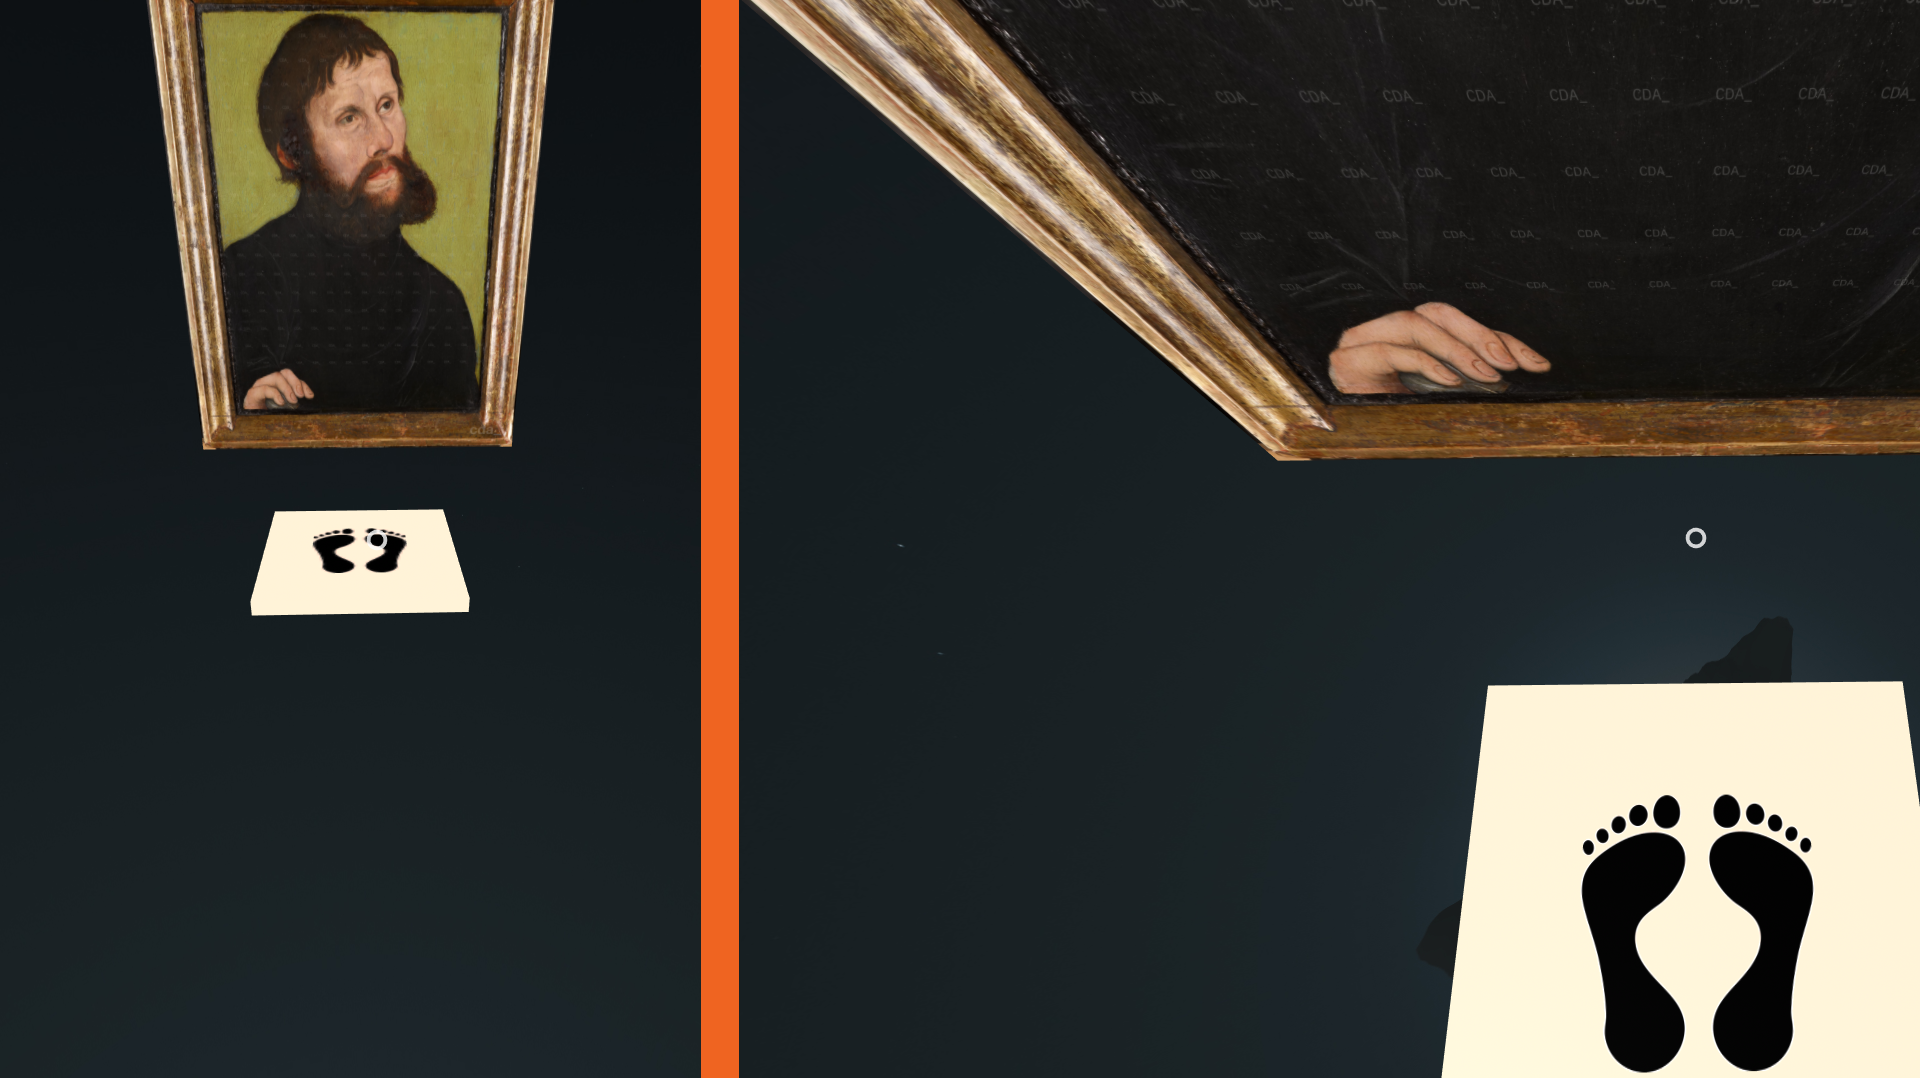
\includegraphics[scale=0.3]{img/coding/standing-area3.png}
          \caption[Funktionsfähige Standing Area zum Teleportieren.]{Funktionsfähige Standing Area zum Teleportieren. [Quelle: Eigene Darstellung].}
          \label{fig:standing-area3}
        \end{figure} \\
        Auf der linken Seite der Abbildung \ref{fig:standing-area3} schaut
        der Benutzer auf die Standing Area, während rechts daneben die neue
        Position des Benutzers dargestellt ist. Er befindet sich
        vor dem Gemälde und kann dieses genauer betrachten. \\
        Zur Gewinnung weiterer Informationen des Gemäldes, wurden
        zusätzlich zur grafischen Darstellung literarische Angaben gemacht.
        Dazu bietet A-Frame das Tag \texttt{<a-text>} an, mit welchem
        zweidimensionale Texte in der virtuellen Welt angezeigt werden können.
        Über das Attribut \texttt{value} wurde der jeweilige Text 
        festgelegt (siehe Abb. \ref{fig:description2}).
        Durch die richtige Positionierung erscheint der Text neben
        dem Gemälde (siehe Abb. \ref{fig:description1}).
        Die Informationen wurden auf den Autor, die Datierung, die Zuschreibung
        und die Bildträger beschränkt.
        \begin{figure}
          \centering
          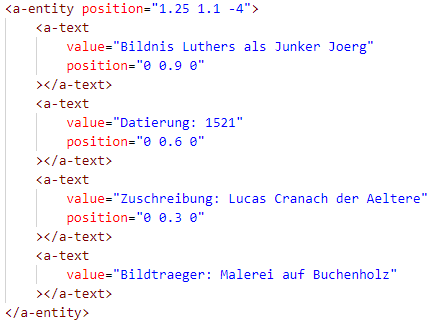
\includegraphics{img/coding/description2.png}
          \caption[Beschreibung zum Gemälde der ID \texttt{DE\_MdbKL\_946}.]{Beschreibung zum Gemälde der ID \texttt{DE\_MdbKL\_946}. [Quelle: Eigene Darstellung].}
          \label{fig:description2}
        \end{figure}        
        \begin{figure}
          \centering
          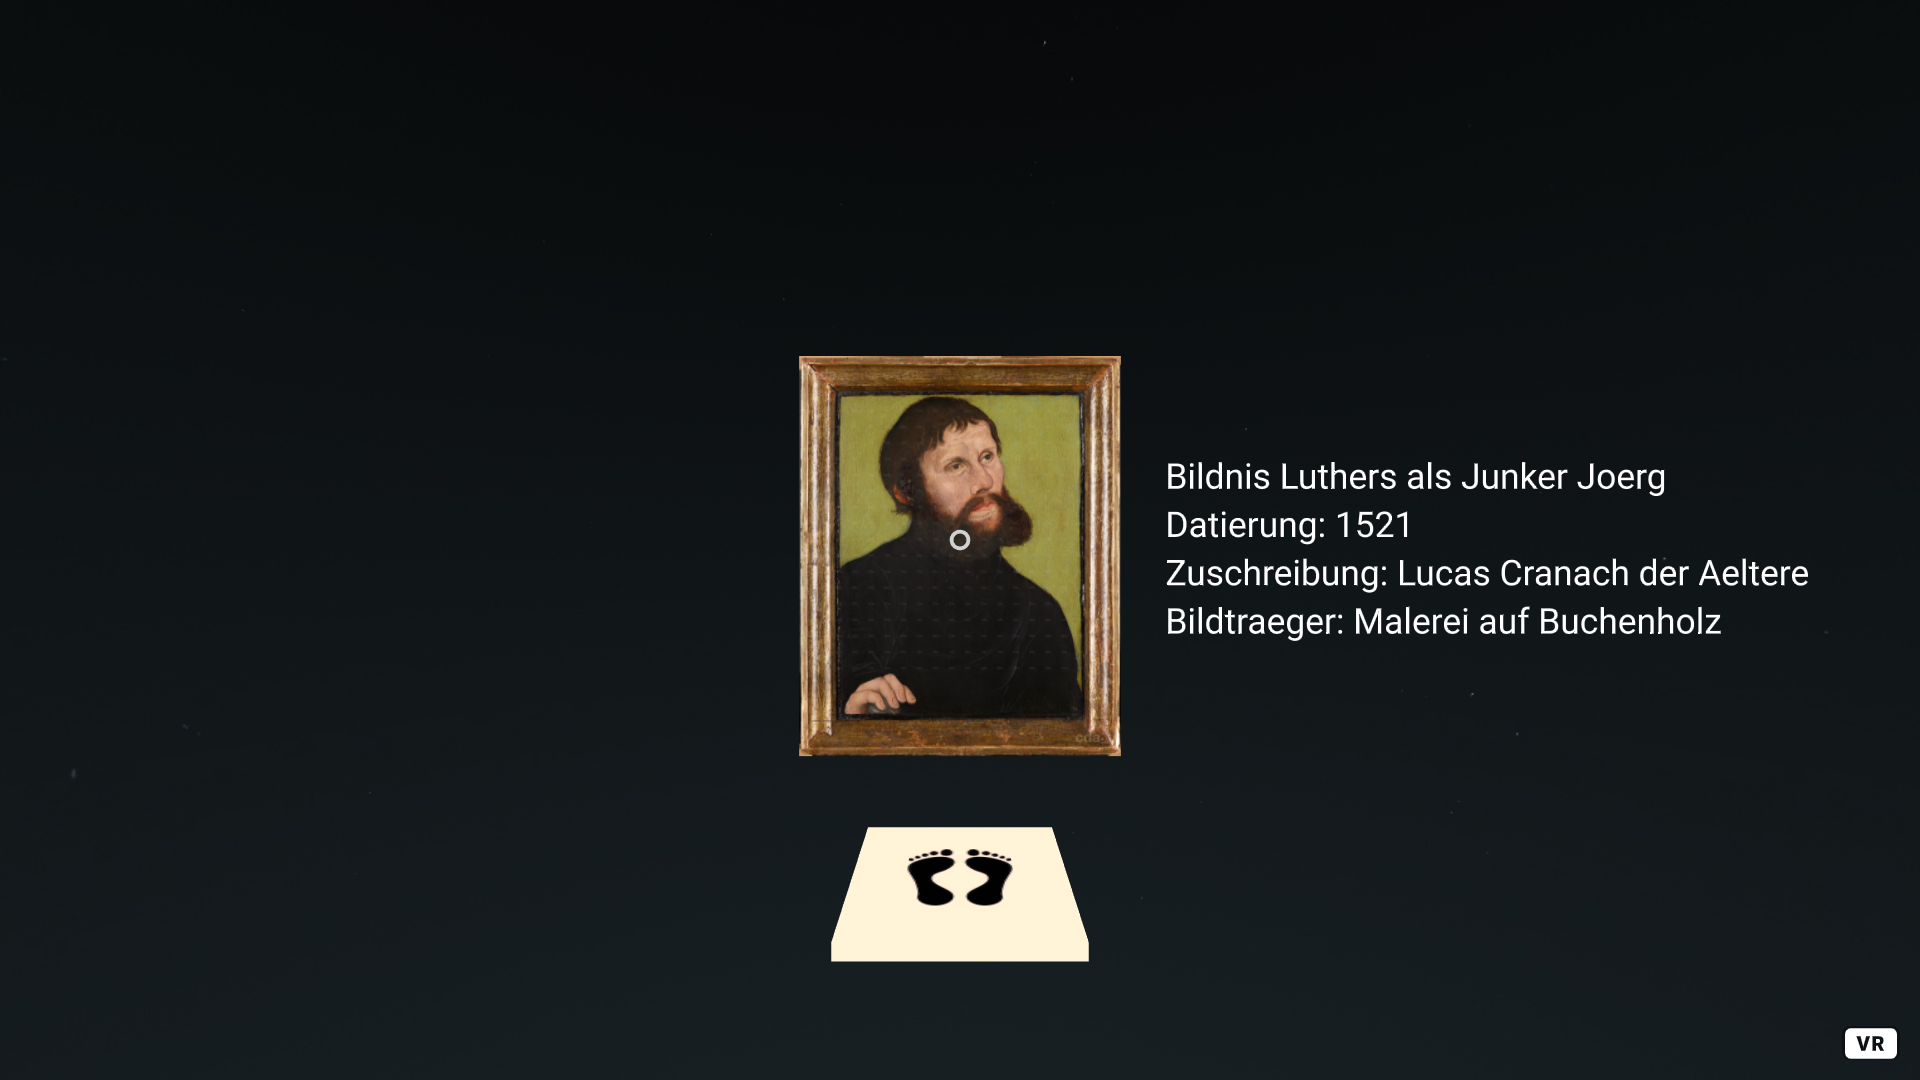
\includegraphics[scale=0.3]{img/coding/description1.png}
          \caption[Beschreibung zum Gemälde der ID \texttt{DE\_MdbKL\_946} innerhalb der virtuellen Welt.]{Beschreibung zum Gemälde der ID \texttt{DE\_MdbKL\_946} innerhalb der virtuellen Welt. [Quelle: Eigene Darstellung].}
          \label{fig:description1}
        \end{figure} \\
        Darüber hinaus lassen sich in Betrachtung des aktuellen 
        Cranach Digital Archives und deren Struktur
        umfangreichere Informationen zusammenfassen 
        (siehe Tabelle \ref{tab:gemaeldeinfos}). Diese wurden für eine
        übersichtlichere Darstellung lediglich durch die Verlinkung
        auf das Cranach Digital Archive angegeben. Da es sich um eine Webanwendung
        handelt und der Benutzer bereits im Browser ist, stellt die Weiterleitung
        kein Problem dar. Wichtig ist dabei die Kennzeichnung zum Öffnen eines
        neuen Fensters, da dies zur Brechung der Ortsillusion 
        aus Kapitel \ref{Wahrnehmungsaspekte} führt.
        \begin{table}[h]
          \begin{center}
          \begin{tabular}{| c |}
            \hline
            \textbf{Gemäldeinformationen} \\ \hline
            Gemälde ID \\ \hline
            Titel \\ \hline
            Zuschreibung \\ \hline
            Datierung \\ \hline
            Eigentümer / Besitzer / Standort \\ \hline
            Maße \\ \hline
            Bildträger \\ \hline
            Signatur / Datierung \\ \hline
            Inschriften / Stempel / Siegel / Beschriftungen \\ \hline
            Kurzbeschreibung \\ \hline
            Provenienz \\ \hline
            Ausstellungen \\ \hline
            Quellen / Publikationen \\ \hline
            Forschungsgeschichte / Diskussion \\ \hline
            Verwandte Arbeiten \\ \hline
            Material / Technik \\ \hline
            Erhaltungszustand \\ \hline
            Restaurierungsgeschichte \\ \hline
          \end{tabular}
          \caption[Informationen eines Gemäldes auf \url{http://lucascranach.org}.]{Informationen eines Gemäldes auf \url{http://lucascranach.org}. [Quelle: Eigene Darstellung].\label{tab:gemaeldeinfos}}
          \end{center}
        \end{table} \\
        Neben den Informationen zu einem Gemälde besitzt dieses im Cranach
        Digital Archive auch mehrere Detailaufnahmen. \\
        Diese zeigen besondere
        Stellen im Gemälde und ermöglichen eine hochauflösende Nahaufnahme.
        Für den Benutzer bietet sich die Möglichkeit diese zusätzlich anzusehen.
        Dafür wurde ein Button unter den Informationen erstellt,
        welcher angeklickt werden kann. Durch das Anklicken dieses Buttons, 
        erscheinen Punkte auf dem Gemälde. Diese wurden an Stelle der 
        jeweiligen Nahaufnahmen positioniert. \\
        Durch das Anklicken einer 
        dieser Punkte, wird das Gemälde durch die jeweilige Nahaufnahme ersetzt. 
        Zur Umsetzung dieser Funktion, wurden zwei weitere Komponenten entwickelt. 
        Zum einen der Button, durch welchen die Punkte innerhalb
        des Gemäldes erscheinen und zum anderen die jeweiligen Punkte, welche
        das Gemälde durch eine Nahaufnahme ersetzen. Dafür verändert die Funktion
        das \texttt{src}-Attribut des Gemäldes. A-Frame reagiert
        auf Veränderungen innerhalb des DOM und aktualisiert die Anwendung
        in Echtzeit. \\
        Der technische Prototyp wurde durch diesen Arbeitsschritt komplexer,
        da mehrere Nahaufnahmen zu einem Gemälde existieren. Somit ist eine
        Datenstruktur für die Gemälde und deren Nahfaunahmen notwendig.
        Zudem haben die Punkte, welche auf dem Gemälde 
        angezeigt werden, ebenfalls eine statische Position innerhalb der
        Gemäldedarstellung. Da die Datenpflege über HTML langfristig 
        zu komplex und
        unübersichtlich wurde, musste diese ausgelagert werden.
        Dafür musste eine Struktur anhand der zur Verfügung stehenden
        Daten entwickelt werden.        
        Um die unterschiedlichen Informationen eines Gemäldes in der Anwendung 
        auslesen zu können, wurden diese im
        JavaScript Object Notation (JSON) Format gespeichert. 
        Dieses Format erlaubt das
        Auslesen von Informationen in JavaScript und anschließend das Speichern dieser
        in JavaScript-Objekte. \\
        Zusammenfassend werden folgende Informationen für
        ein Gemälde innerhalb einer virtuellen Welt zur Darstellung benötigt
        (siehe Abb. \ref{fig:json-aufbau1}).
        \begin{figure}[h]
          \centering
          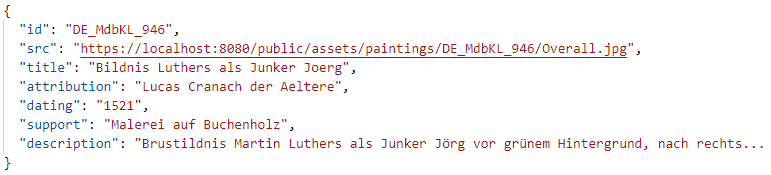
\includegraphics[scale=0.8]{img/coding/json-aufbau1.png}
          \caption[JSON-Struktur eines Gemäldes.]{JSON-Struktur eines Gemäldes. [Quelle: Eigene Darstellung].}
          \label{fig:json-aufbau1}
        \end{figure} \\
        Da JavaScript beim Auslesen einer JSON-Datei nicht wissen kann,
        um was für einen Objekttypen es sich handelt, wurde zusätzlich ein
        Interface in TypeScript angelegt. \\
        Dieser bietet innerhalb des Codes Typsicherheit sowie eine
        verbesserte Unterstützung der Code Completion innerhalb der
        Entwicklungsumgebung (siehe Abb. \ref{fig:painting-type1}).
        \begin{figure}[h]
          \centering
          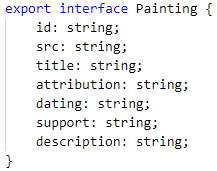
\includegraphics{img/coding/painting-type1.png}
          \caption[Gemälde-Interface in TypeScript.]{Gemälde-Interface in TypeScript. [Quelle: Eigene Darstellung].}
          \label{fig:painting-type1}
        \end{figure} \\
        Um ein Gemälde anhand einer JSON-Datei darzustellen,
        muss das Generieren vollständig auf JavaScript
        basieren, da das dynamische Auslesen aller Informationen
        nicht im HTML umgesetzt werden kann. 
        Dafür wurde eine 
        Komponente entwickelt,
        welche die JSON-Datei ausliest und anhand dieser Daten ein Gemälde
        in Kombination mit dessen Informationen und Nahaufnahme-Buttons generiert. \\
        Die Komponente \texttt{paintings-builder} wurde der 
        \texttt{<a-scene>} hinzugefügt, da
        diese beim Erstellen der VR-Szene ausgeführt werden soll. Die
        Komponente wurde im Plural geschrieben, da die Option freigehalten
        werden soll, mehrere Gemälde generieren zu können. \\
        Durch die \texttt{init}-Methode wird in der Komponente zuerst 
        die JSON-Datei ausgelesen und anschließend \texttt{createPainting(...)}
        ausgeführt (siehe Abb. \ref{fig:paintings-builder1}).
        Diese Methode bekommt ein Objekt des Typs \texttt{Painting}
        (Typdefinition siehe Abb. \ref{fig:painting-type1}). \\ 
        In Abbildung
        \ref{fig:json-aufbau1} befinden sich in der JSON-Datei die Informationen
        zu lediglich einem Gemälde. Der Code kann jedoch mehrere Gemälde 
        entgegennehmen.
        \begin{figure}[b]
          \centering
          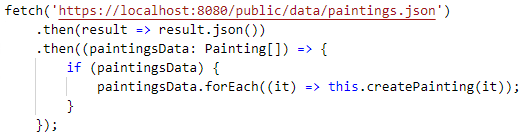
\includegraphics{img/coding/paintings-builder1.png}
          \caption[Abrufen der Daten aus der \texttt{paintings.json} und Ausführen der \texttt{createPainting}-Methode.]{Abrufen der Daten aus der \texttt{paintings.json} und Ausführen der \texttt{createPainting}-Methode. [Quelle: Eigene Darstellung].}
          \label{fig:paintings-builder1}
        \end{figure} 
        Innerhalb der \texttt{createPainting}-Methode wird das Gemälde,
        die Informationen und die Standing Area erzeugt. 
        Bei der Standing Area handelt es sich um 
        das in Abbildung \ref{fig:standing-area1} dargestellte HTML, 
        welches in das JavaScript übersetzt und eingefügt wurde.
        Da jedes Gemälde eine Standing Area benötigt,
        wurde diese immer mit einem Gemälde zusammen generiert.
        Für das weitere Verständnis im Rahmen dieser Forschungsarbeit
        ist die vollständige Erläuterung der 
        \texttt{paintings-builder}-Komponente nicht notwendig,
        sodass im Folgenden auf weitere Beschreibungen verzichtet wird. \\
        Die relevantesten Codestellen innerhalb der 
        \texttt{paintings-builder} sind jene, welche das Gemälde und
        dessen Informationen generieren (siehe Abb. \ref{fig:paintings-builder2}).
        \begin{figure}
          \centering
          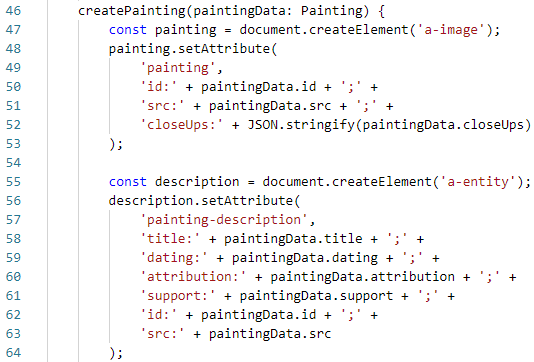
\includegraphics{img/coding/paintings-builder2.png}
          \caption[Codeabschnitt für die Generierung des Gemäldes und dessen Informationen.]{Codeabschnitt für die Generierung des Gemäldes und dessen Informationen. [Quelle: Eigene Darstellung].}
          \label{fig:paintings-builder2}
        \end{figure}
        Das \text{<a-image>}-Tag bekommt dabei eine Komponente 
        namens \texttt{painting} während die Informationen zum Gemälde
        eine Komponente mit dem Titel
        \texttt{painting-description} bekommen. Die Informationen werden
        weiterhin gemeinsam in einem \texttt{<a-entity>}-Tag gebündelt.
        Beide Komponenten bekommen darüber hinaus
        die notwendigen Informationen über ihr Schema
        (siehe Abb. \ref{fig:paintings-builder2}, Zeile 48-53 und Zeile 56-64).
        So wird kein HTML benötigt und die Daten können dynamisch ausgelesen
        und in die einzelnen Komponenten hineingegeben werden. \\
        Die \texttt{painting}-Komponente bekommt neben ihrer eigenen Gemälde-ID
        und deren Pfad zur Bilddatei weitere Informationen der einzelnen
        Nahaufnahmen, da diese innerhalb des Gemäldes generiert werden. \\
        In der \texttt{init}-Methode dieser Komponente wird die 
        \texttt{createDetailPoints}-Methode aufgerufen 
        (siehe Abb. \ref{fig:painting1}).
        \begin{figure}
          \centering
          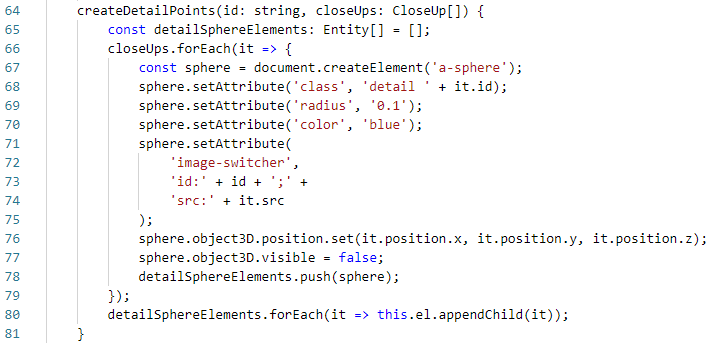
\includegraphics{img/coding/painting1.png}
          \caption[\texttt{createDetailPoints} innerhalb der \texttt{painting}-Komponente.]{\texttt{createDetailPoints} innerhalb der \texttt{painting}-Komponente. [Quelle: Eigene Darstellung].}
          \label{fig:painting1}
        \end{figure}
        Diese nimmt folgende Argumente entgegen: \texttt{id: string} und
        \texttt{closeUps: CloseUp[]}. Die \texttt{id} des Gemäldes wird
        innerhalb der \texttt{image-switcher} Komponente benötigt
        (siehe Abb. \ref{fig:painting1}, Zeile 74-75). 
        Die Informationen der Nahaufnahmen sind in dem Parameter 
        \texttt{closeUps} gespeichert. Dieses Objekt beinhaltet neben
        der \texttt{id} und \texttt{src} auch die Positionen der Punkte
        relativ zum Gemälde. \\ \\
        In der \texttt{image-switcher}-Komponente
        wird der \texttt{click}-EventListener registriert, welcher bei
        einem Klick das Gemälde mit einer Nahaufnahme ersetzt und die 
        aktivierten Punkte ausblendet. Durch
        \texttt{visible = false} werden die Punkte initial unsichtbar gestellt
        (siehe Abb. \ref{fig:painting1}, Zeile 83). \\
        Die \texttt{painting-description}-Komponente aus Abbildung 
        \ref{fig:paintings-builder2} hat sich nicht deutlich
        zu der HTML-Version aus Abbildung \ref{fig:description2} verändert. 
        So wurde zusätzlich
        eine \texttt{<a-box>} generiert, welche den Button darstellt.
        Dieser Button erhält eine Komponente namens \texttt{detail-button}, welche
        bei Klicken das Anzeigen der jeweiligen Nahaufnahmen ermöglicht.
        Dabei erhält der Button den Schriftzug \glqq Zurück\grqq{}, 
        um von der Nahaufnahme zum Gemälde umzuschalten. \\
        Der erste Prototyp umfasst abschließend die Anzeige des
        jeweiligen Gemäldes und dessen Informationen in Kombination mit
        einem Detail-Button (siehe Abb. \ref{fig:paintings-builder3}).
        \begin{figure}
          \centering
          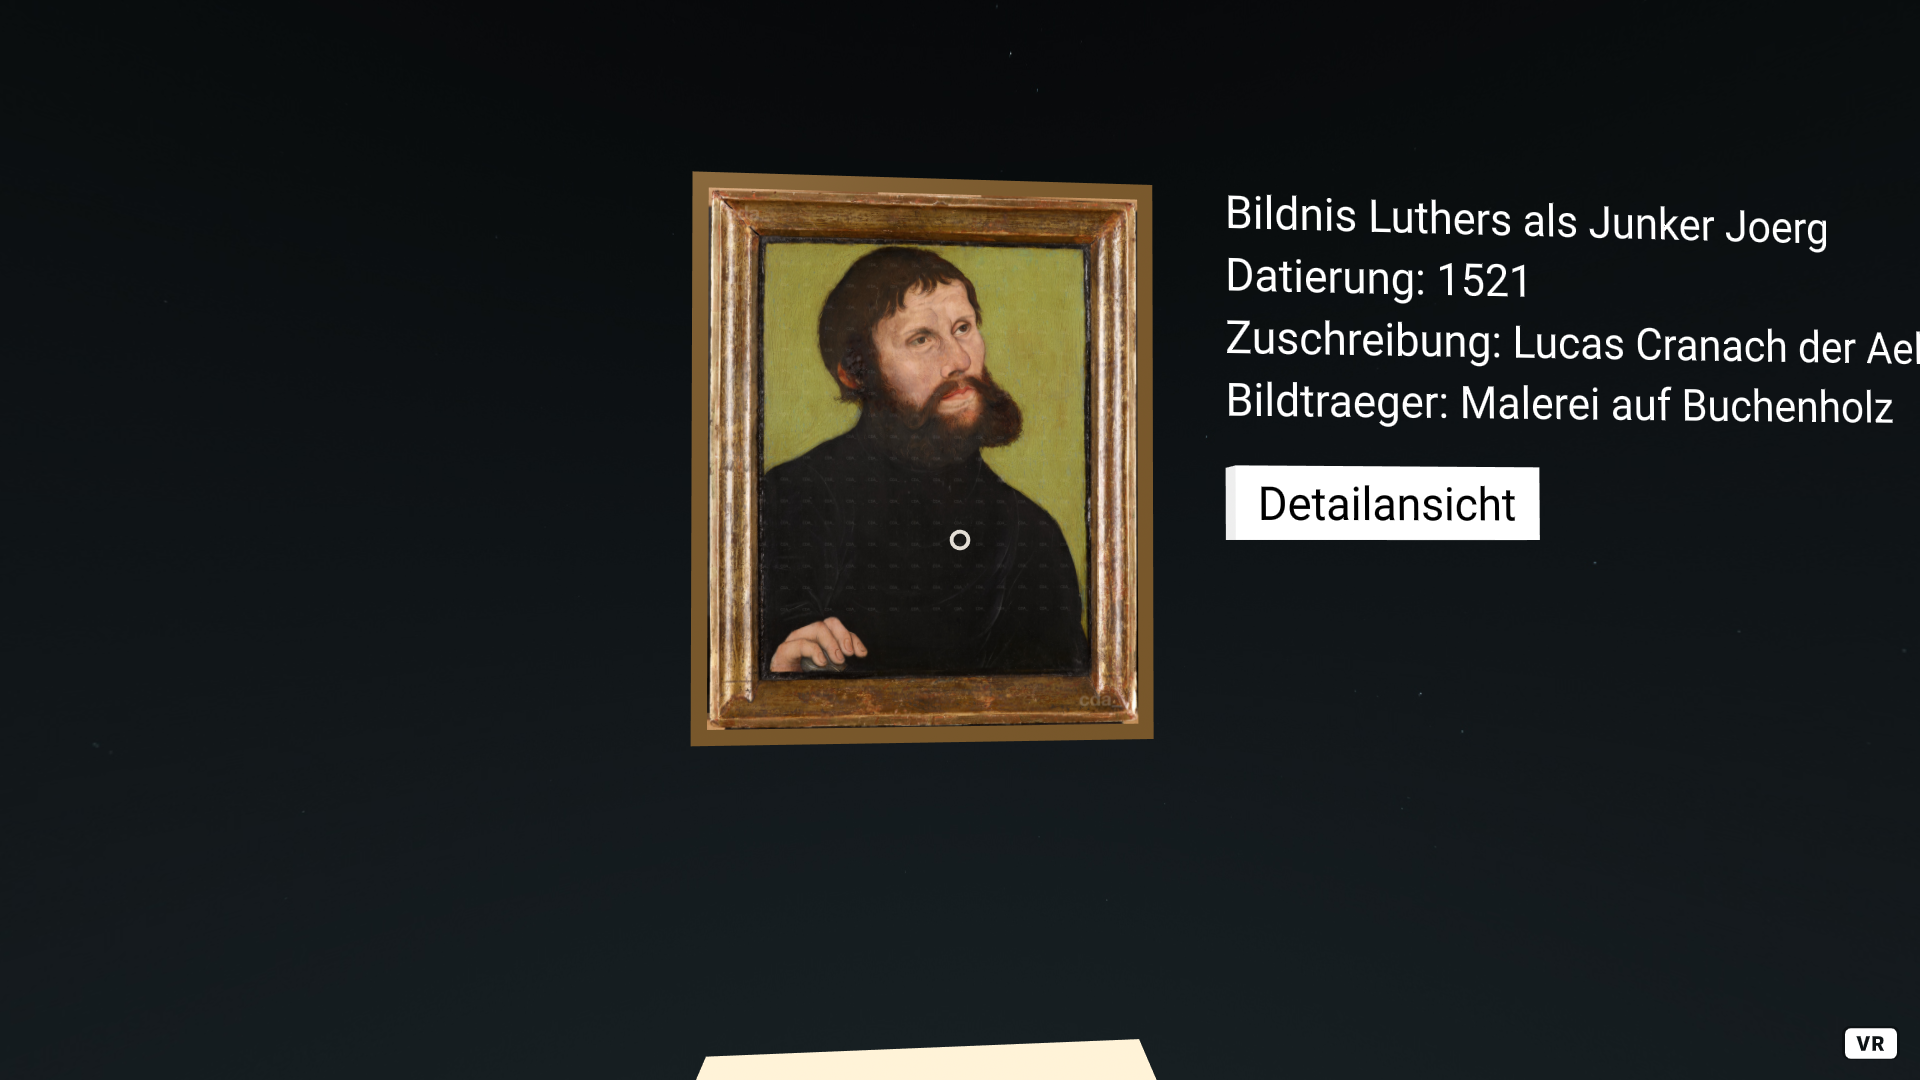
\includegraphics[scale=0.3]{img/coding/paintings-builder3.png}
          \caption[Ansicht des ersten fertigen Prototypen.]{Ansicht des ersten fertigen Prototypen. [Quelle: Eigene Darstellung].}
          \label{fig:paintings-builder3}
        \end{figure}
        Klickt der Benutzer demnach auf den Button \glqq Detailansicht\grqq{},
        erscheinen blaue Punkte auf dem Gemälde
        (siehe Abb. \ref{fig:paintings-builder4}).
        \begin{figure}
          \centering
          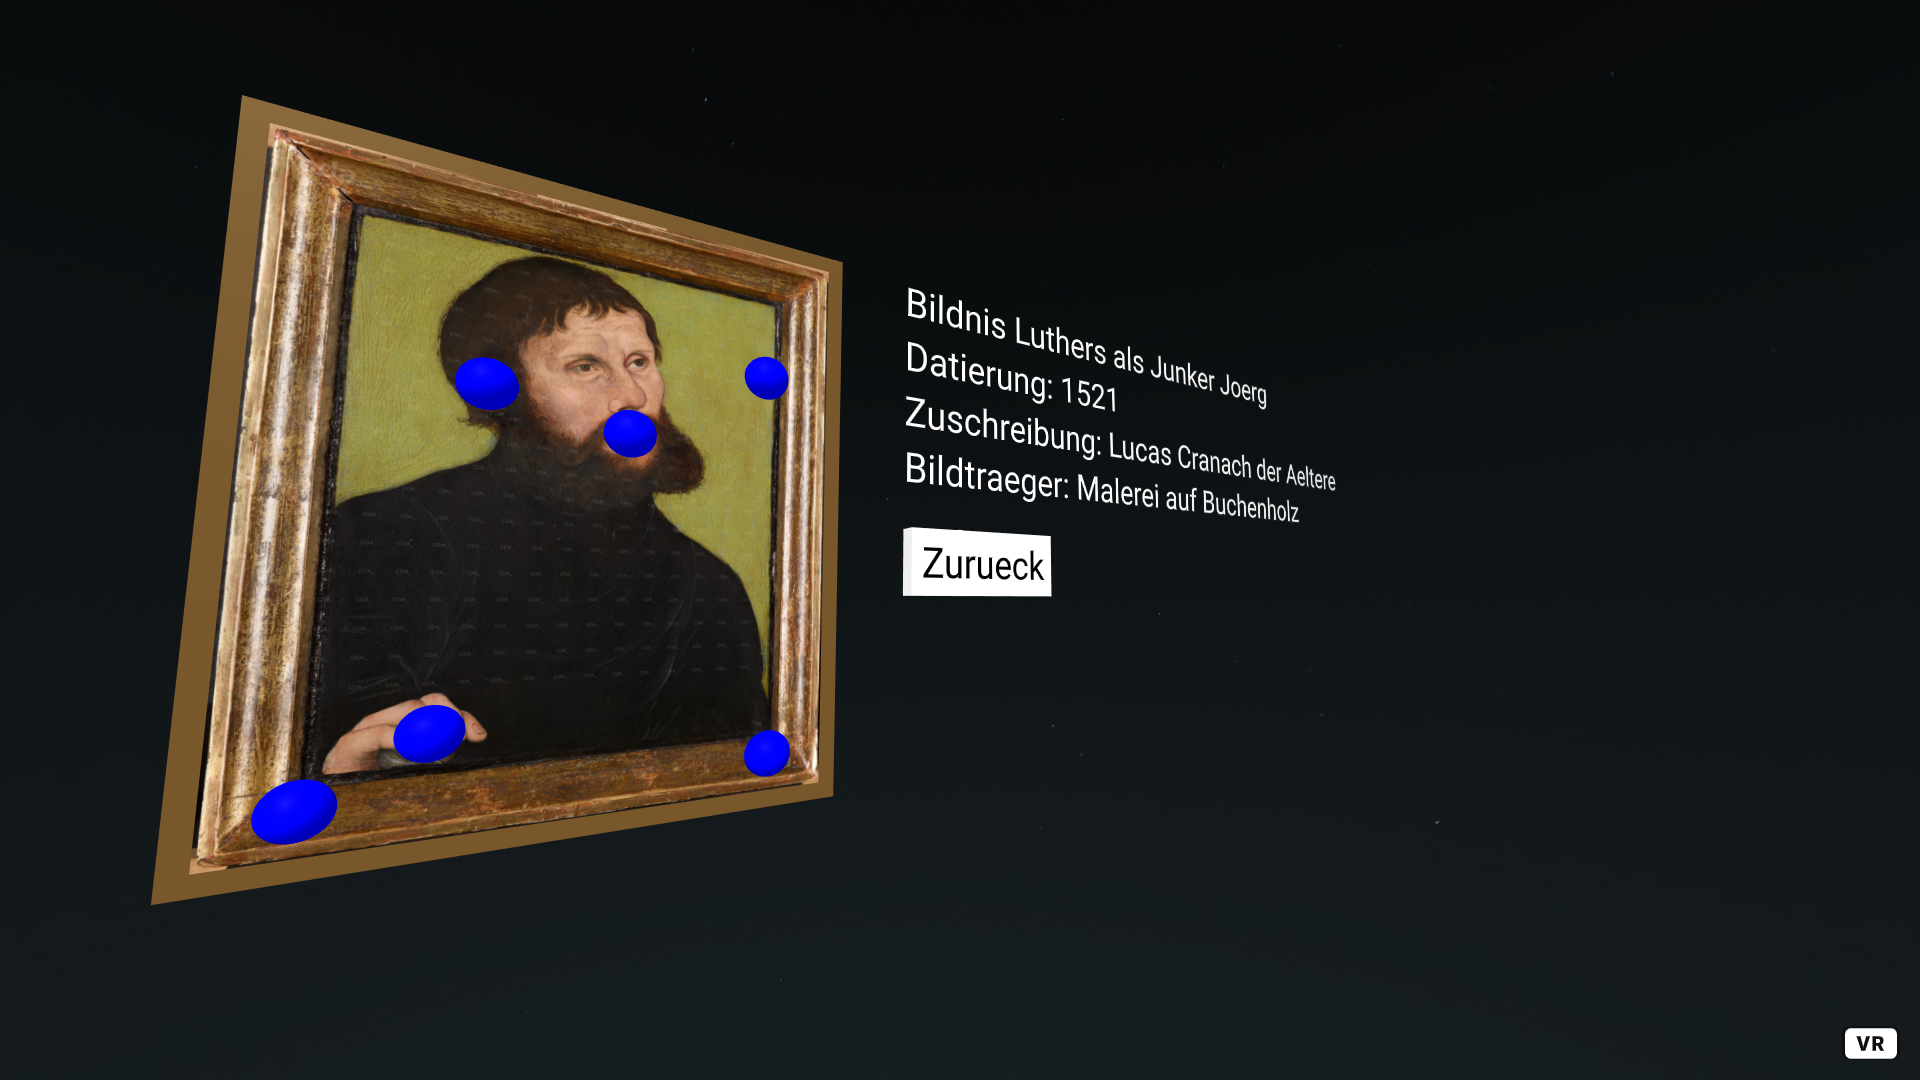
\includegraphics[scale=0.3]{img/coding/paintings-builder4.png}
          \caption[Detailpunkte auf dem Gemälde nach einem Klick auf den \glqq Detailansicht\grqq{}-Button.]{Detailpunkte auf dem Gemälde nach einem Klick auf den \glqq Detailansicht\grqq{}-Button. [Quelle: Eigene Darstellung.]}
          \label{fig:paintings-builder4}
        \end{figure}
        Durch einen weiteren Klick auf einer der Punkte, wird das
        aktuelle Gemälde durch eine Nahaufnahme ersetzt
        (siehe Abb. \ref{fig:paintings-builder5}).
        \begin{figure}
          \centering
          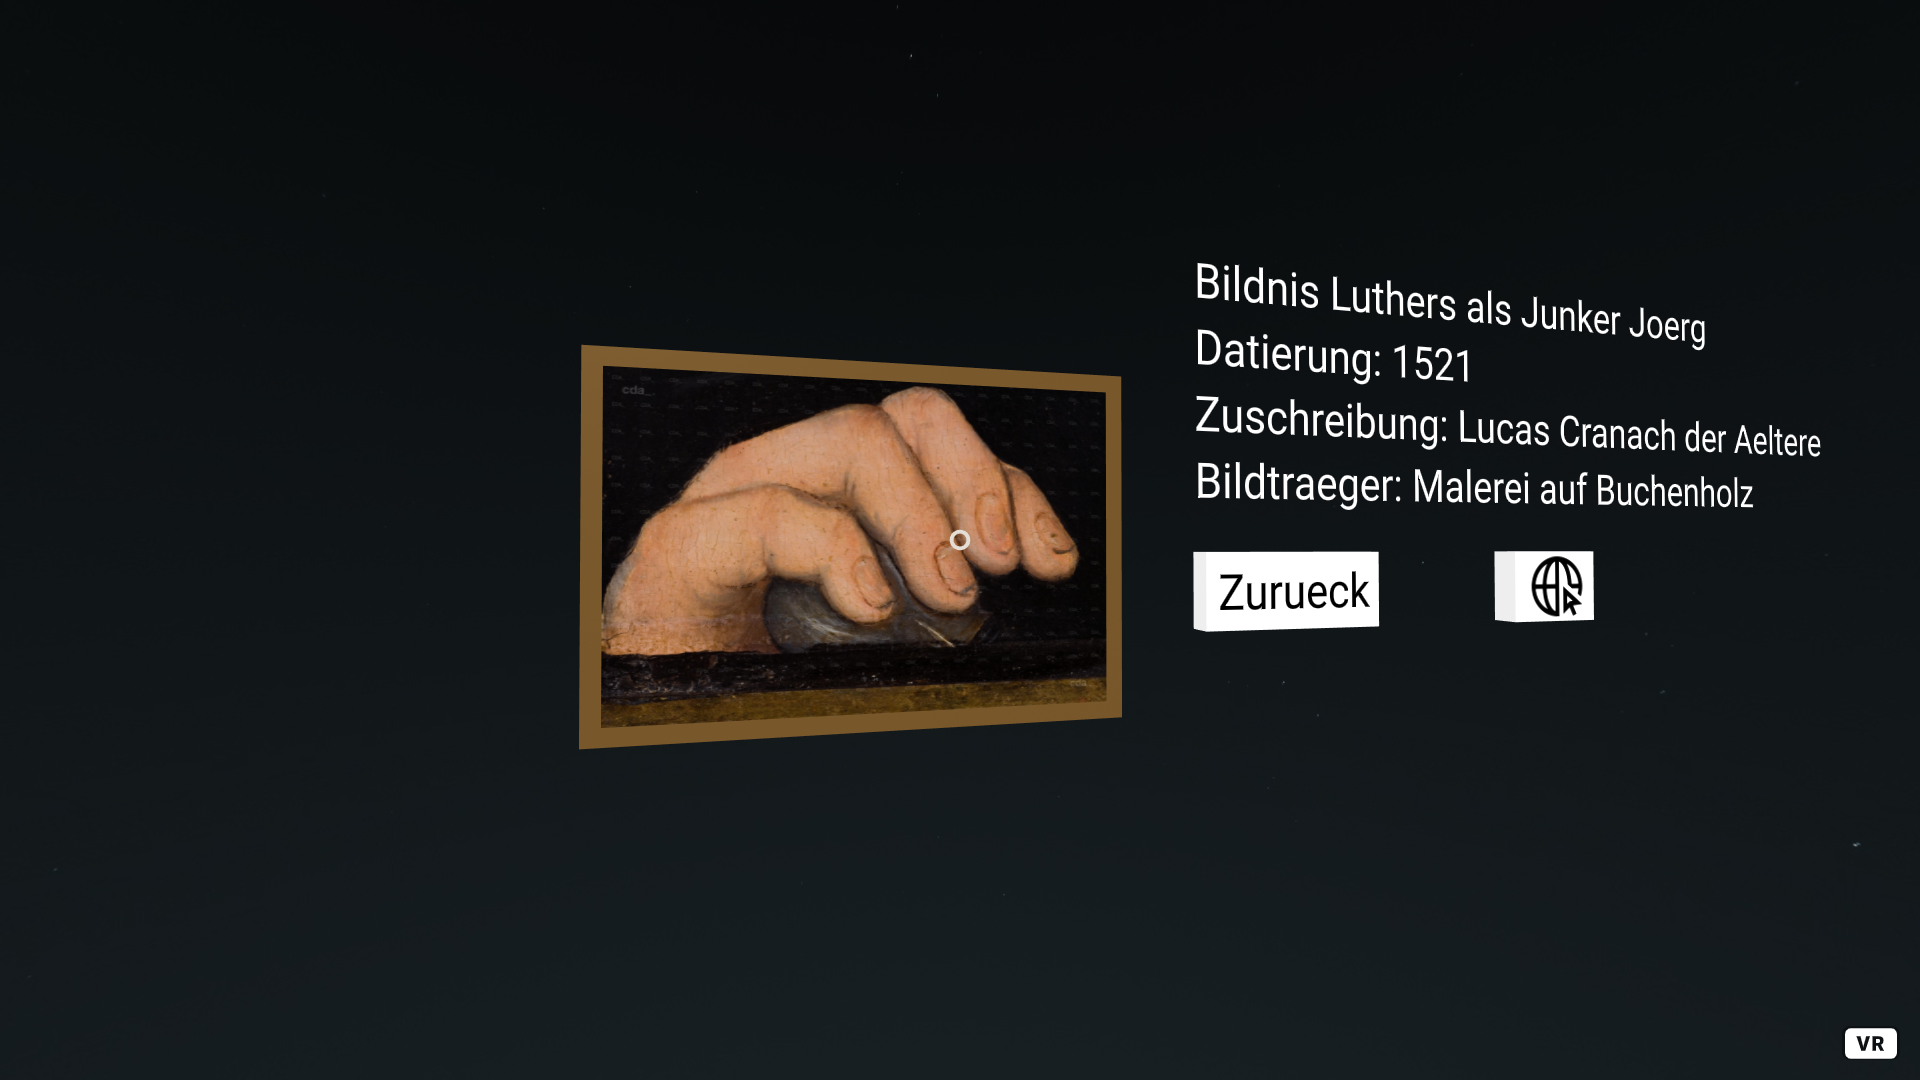
\includegraphics[scale=0.3]{img/coding/paintings-builder5.png}
          \caption[Eine Nahaufnahme des Gemäldes mit der ID \texttt{DE\_MdbKL\_946}.]{Eine Nahaufnahme des Gemäldes mit der ID \texttt{DE\_MdbKL\_946}. [Quelle: Eigene Darstellung].}
          \label{fig:paintings-builder5}
        \end{figure} \\
        Darüber hinaus bildet der erste technische Prototyp das Fundament
        der weiteren Prototypen. Durch das komponentenbasierte System von
        A-Frame lässt sich diese Art der Darstellung in andere Szenen
        und in einem anderen Kontext wiederverwenden. \newpage
      \subsubsection{Lucas Cranachs Werkstatt}
        Cranach entwarf viele seiner Gemälde in seiner
        eigenen Werkstatt. Diese bildet die Grundlage 
        des zweiten Prototypen, in welchem der Benutzer in 
        ein Szenario aus der Vergangenheit
        versetzt wird. 
        Durch die Archivierung unterschiedlicher Gemälde 
        und anderer Dokumente ist es möglich, gewisse Tage
        von Cranach zu rekonstruieren. So wurde ein
        Gemälde mit einem schriftlichen Dokument aus
        dem selben Jahr zusammengefügt, um ein umfangreicheres
        Wissen zu vermitteln. Die Schrift des Dokumentes
        ist für den Benutzer unleserlich. Durch einen Klick
        auf einen Button wird die Beschreibung aus dem Cranach
        Digital Archive zu diesem Dokument akustisch vorgetragen. \\
        Um diese Werkstatt als Szene in A-Frame umzusetzen, wurden 3D-Modelle
        verwendet. Nach einer kurzen Recherche bei Google haben sich
        Poly von Google\footnote{Poly von Google | \url{https://poly.google.com/} (22.11.2020).}
        und Sketchfab\footnote{Sketchfab | \url{https://sketchfab.com/} (22.11.2020).}
        als Plattformen für kostenfreie 3D-Modelle hervorgehoben. \\
        A-Frame bietet die Möglichkeit, ganze 3D-Modelle über einen
        HTML-Tag einzubinden. Dabei erlaubt das Framework die Einbindung von
        mehreren Datentypen. In diesem Projekt
        wurde sich für glTF entschieden, da dieser Dateityp eine 
        royalty-free Spezifikation für 3D-Modelle ist. Zudem kann glTF als leichtgewichtig 
        und interoperabel angesprochen werden\footnote{glTF Overview | \url{https://www.khronos.org/gltf/} (22.11.2020).}.
        Sketchfab wie auch Poly bieten glTF als Dateiformat an. \\
        Das Einbinden eines glTF-Modells erfolgt über das A-Frame-Tag 
        \texttt{\textbf{<a-gltf-model>}}. Das Modell lässt sich über das Attribut
        \texttt{src} einbinden. Wie auch bei Bildern, kann der Pfad oder die ID
        aus dem \texttt{<a-assets>}-Tag verwendet werden. 
        Für die Einbindung des 3D-Modells über \texttt{<a-assets>} wurde dieses
        darin als \texttt{<a-asset-item>} hinzugefügt.
        Die Abbildung \ref{fig:gltf1} zeigt, wie ein glTF-Modell 
        eingefügt werden kann.
        \begin{figure}
          \centering
          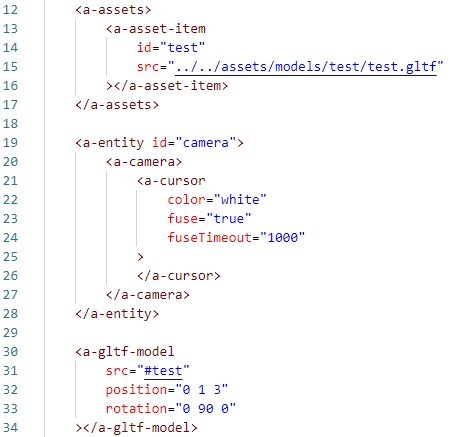
\includegraphics{img/coding/gltf1.png}
          \caption[Einbinden eines glTF-Modells in A-Frame über \texttt{<a-assets>}.]{Einbinden eines glTF-Modells in A-Frame über \texttt{<a-assets>}. [Quelle: Eigene Darstellung].}
          \label{fig:gltf1}
        \end{figure} \\
        Komponenten wie \texttt{painting}, \texttt{painting-description} und 
        \texttt{standing-area} wurden in diesem Prototypen wiederverwendet. 
        Ein lediglicher Mehraufwand entstand durch die Modellierung
        der Werkstatt.
        Durch die mögliche Nutzung fertiger und kostenfreier Modelle
        von Poly und Sketchfab, entfiel der 
        Arbeitsschritt des Modellierens eigener Modelle. \\
        Die Werkstatt wurde mittels A-Frame-Editor, welcher mit \texttt{STRG + ALT + I}
        innerhalb der Webanwendung aufgerufen werden kann, gestaltet. \\
        Grundlegend besteht die Werkstatt aus zwei Bereichen. Zum einen 
        aus dem Bereich der grafischen Darstellung des Gemäldes
        (siehe Abb. \ref{fig:werkstatt2}),
        zum anderen aus dem Bereich der visuellen und akustischen 
        Darstellung der schriftlichen Dokumente
        (siehe Abb. \ref{fig:werkstatt1}).
        \begin{figure}
          \centering
          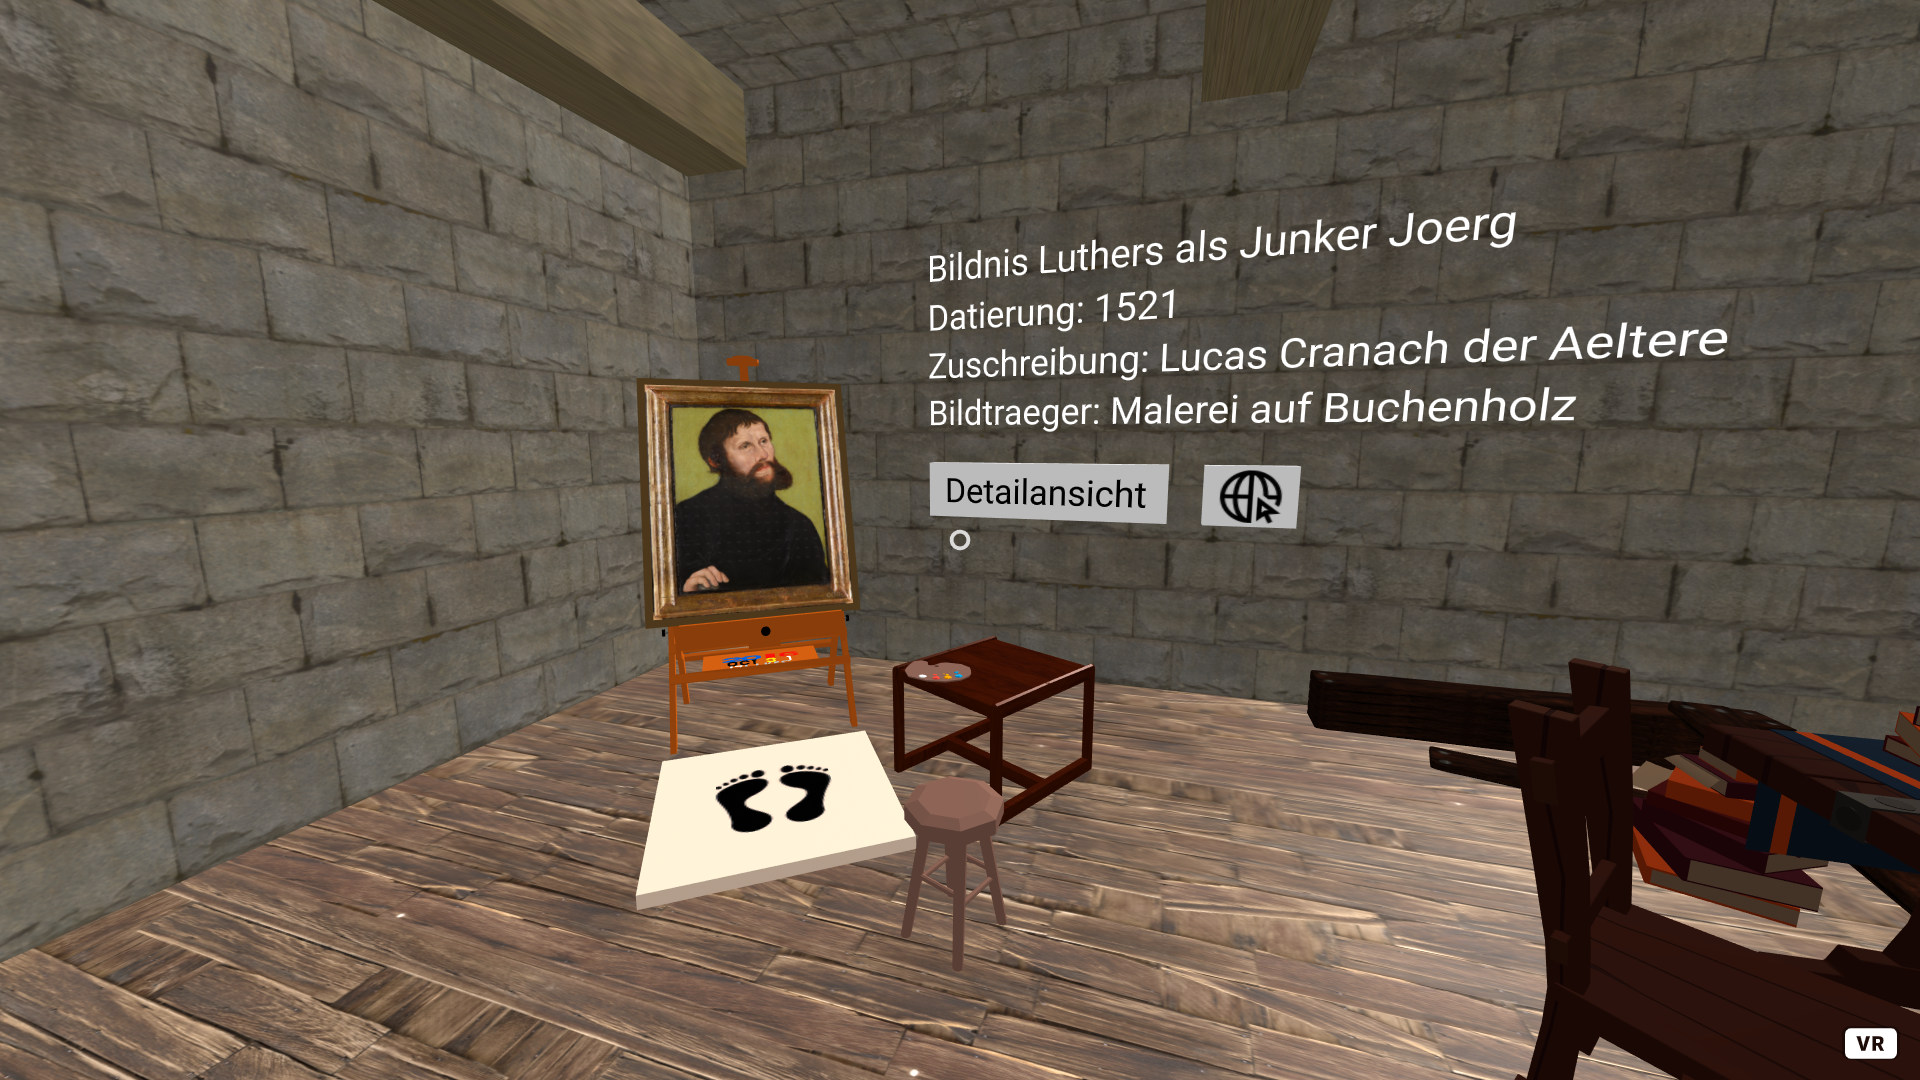
\includegraphics[scale=0.3]{img/coding/werkstatt2.png}
          \caption[Gemälde (1521) von Cranach in seiner fiktiven Werkstatt.]{Gemälde (1521) von Cranach in seiner fiktiven Werkstatt. [Quelle: Eigene Darstellung].}
          \label{fig:werkstatt2}
        \end{figure}
        \begin{figure}
          \centering
          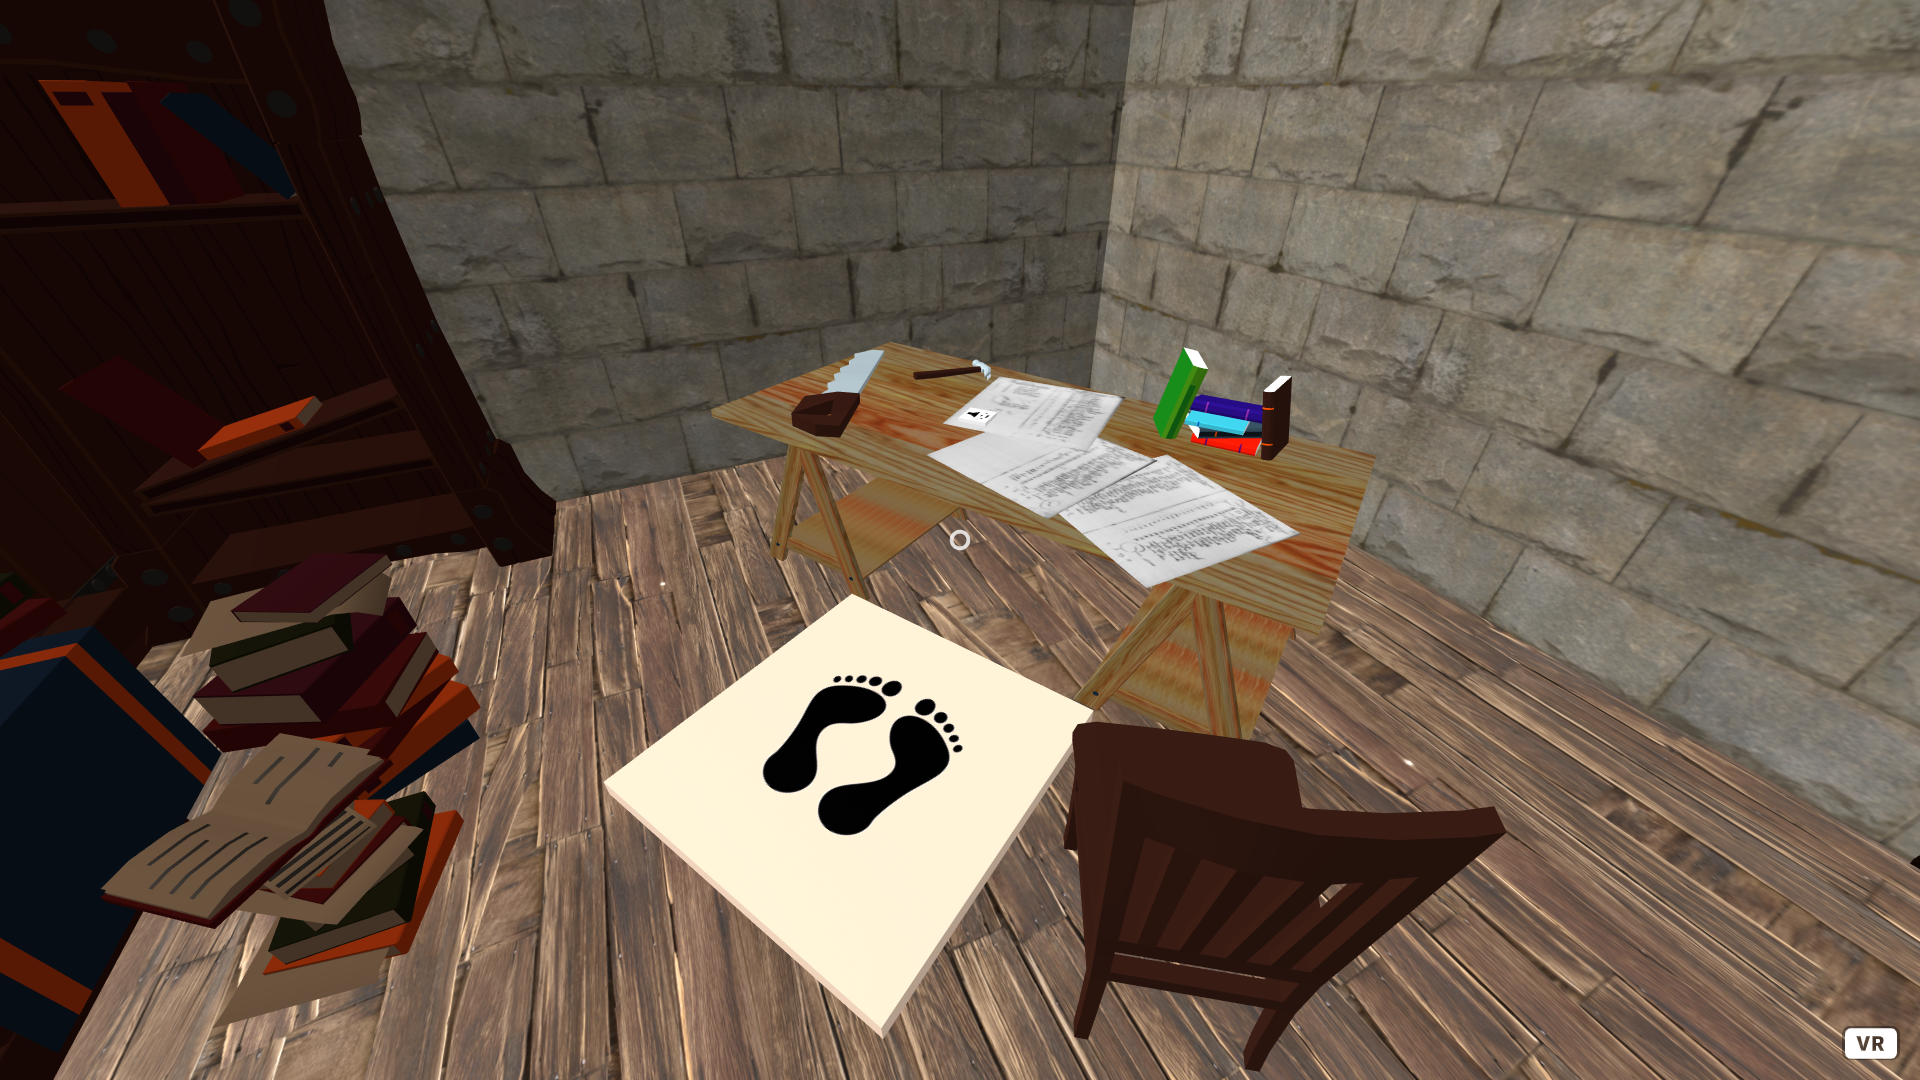
\includegraphics[scale=0.3]{img/coding/werkstatt1.png}
          \caption[Dokumente (1521) von Cranach in seiner fiktiven Werkstatt.]{Dokumente (1521) von Cranach in seiner fiktiven Werkstatt. [Quelle: Eigene Darstellung].}
          \label{fig:werkstatt1}
        \end{figure} \\
        Der Benutzer kann über die Standing Area zu den jeweiligen Bereichen
        teleportiert werden. \\
        In Abbildung \ref{fig:werkstatt2} sind
        zusätzlich die
        Komponenten \texttt{painting} und \texttt{painting-description},
        welche im letzten Kapitel beschrieben und entwickelt 
        wurden, erkennbar. Die Beschreibung des
        Gemäldes befindet sich an der Wand der Werkstatt 
        und kann dort auf Augenhöhe von
        dem Benutzer erkannt werden. Die ebenfalls
        zuvor beschriebenen Detailaufnahmen können
        zusätzlich betrachtet werden. \\
        Teleportiert sich der Benutzer zu dem Bereich der Dokumente, 
        die über mehrere Seiten verteilt auf einem Tisch liegen,
        kann er diese visuell und akustisch erfahren. \\
        Über einen Button, welcher
        sich auf einem der Dokumente befindet, kann die 
        jeweilige Beschreibung angehört werden
        (siehe Abb. \ref{fig:werkstatt3}).
        \begin{figure}
          \centering
          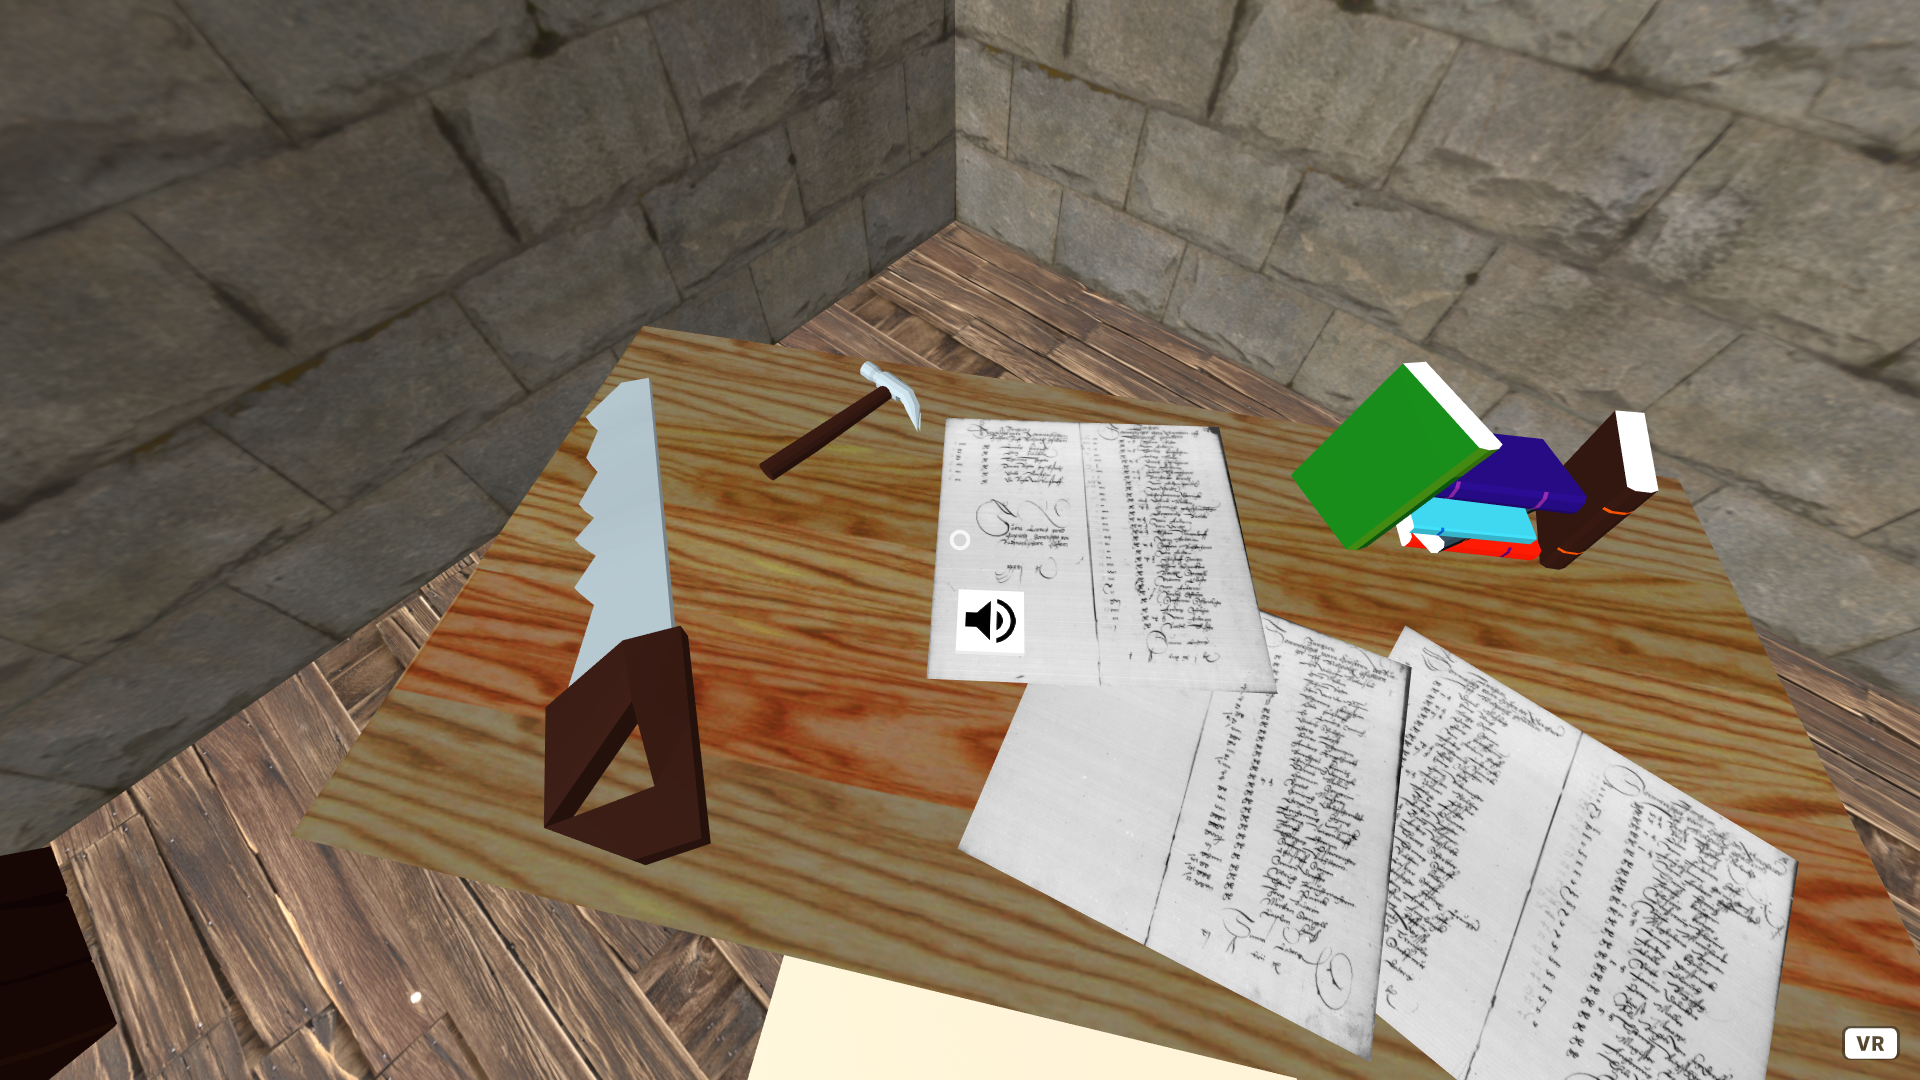
\includegraphics[scale=0.3]{img/coding/werkstatt3.png}
          \caption[Sound-Button der Dokumente von Cranach in seiner fiktiven Werkstatt.]{Sound-Button der Dokumente von Cranach in seiner fiktiven Werkstatt. [Quelle: Eigene Darstellung].}
          \label{fig:werkstatt3}
        \end{figure} \\
        Die Darstellung der Dokumente von Cranach wird über die
        neue Komponente \texttt{document} ermöglicht. Diese nimmt über das
        Schema die Eigenschaften \texttt{id} und \texttt{page} 
        entgegen (siehe Abb. \ref{fig:document1}).
        Durch die Eigenschaft \texttt{page} wurden verschiedene
        Darstellungen eines Dokuments der selben ID ermöglicht. Über das
        \texttt{<audio>}-Tag wurden in \texttt{<a-assets>} Sounddateien der
        Anwendung hinzugefügt. A-Frame bietet dazu die Möglichkeit, 
        mehrere Dateiformate anzunehmen und wiederzugeben. 
        Dabei hat jedes Dokument die mögliche Funktion
        einen Soundbutton darzustellen.
        Dies ist abhängig davon, ob das
        Dokument eine Sound-Entität als \texttt{children}-Element besitzt
        (siehe Abb. \ref{fig:document1}, Zeile 92).
        \begin{figure}
          \centering
          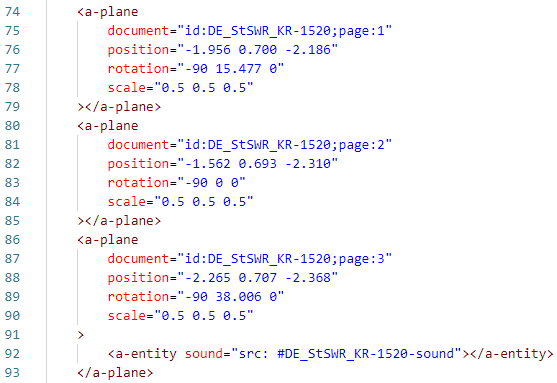
\includegraphics{img/coding/document1.png}
          \caption[\texttt{document}-Komponente als HTML-Implementation.]{\texttt{document}-Komponente als HTML-Implementation. [Quelle: Eigene Darstellung].}
          \label{fig:document1}
        \end{figure}
        So wird innerhalb der Komponente abgefragt, ob diese über 
        eine Sound-Entität verfügt. Sofern dies der Fall ist, 
        wird der Sound-Button angezeigt. \newpage
      \subsubsection{Neuronales Netz}
        Bei dem letzten Prototypen handelt es sich um eine Darstellung, die
        einem neuronalen Netz ähnelt. In diesem wurde die Beziehung
        zwischen den Gemälden und den jeweiligen Nahaufnahmen dargestellt.
        Grundlage dieses Prototypen sind alle verfügbaren
        Gemälde von Martin Luther als Junker Jörg des Cranach Digital
        Archives. Diese sind nachweislich miteinander verwandt und 
        dienen daher als vergleichbare Datenbasis.
        Die einzelnen Nahaufnahmen können durchgehend einem 
        Gemälde zugeordnet werden. \\
        In einem neuronalen Netz werden Verbindungen meist durch eine
        einfache Linie dargestellt. A-Frame bietet dabei die Möglichkeit
        mit \texttt{<a-entity line=\dq start: x, y, z; end: x, y, z;\dq{}>} eine
        Linie zu zeichnen. Dabei muss ein Start- und Endpunkt in der
        virtuellen Welt angegeben werden. Zusätzlich lässt sich durch
        das Attribut \texttt{color} eine Farbe für die Linie angeben. \\
        Um diesen Prototypen zu entwickeln, wurde auf die Komponente
        \texttt{painting} zurückgegriffen. Die Nahaufnahmen
        sind daraufhin zu jedem Zeitpunkt sichtbar und müssen nicht mehr
        durch den Klick auf einen Button angezeigt werden. \\
        Somit
        können die Nahaufnahmen ebenfalls die \texttt{painting}-Komponente
        verwenden, um eine Darstellung in der virtuellen Welt dauerhaft
        zu erhalten. \\
        Die roten Linien in Abbildung \ref{fig:neural-network1} 
        stellen die Verbindungen von einem Gemälde zu
        einer Nahaufnahme dar, während die blauen Linien die thematische
        Verbindung zwischen den unterschiedlichen Gemälden verdeutlicht. 
        \begin{figure}[h]
          \centering
          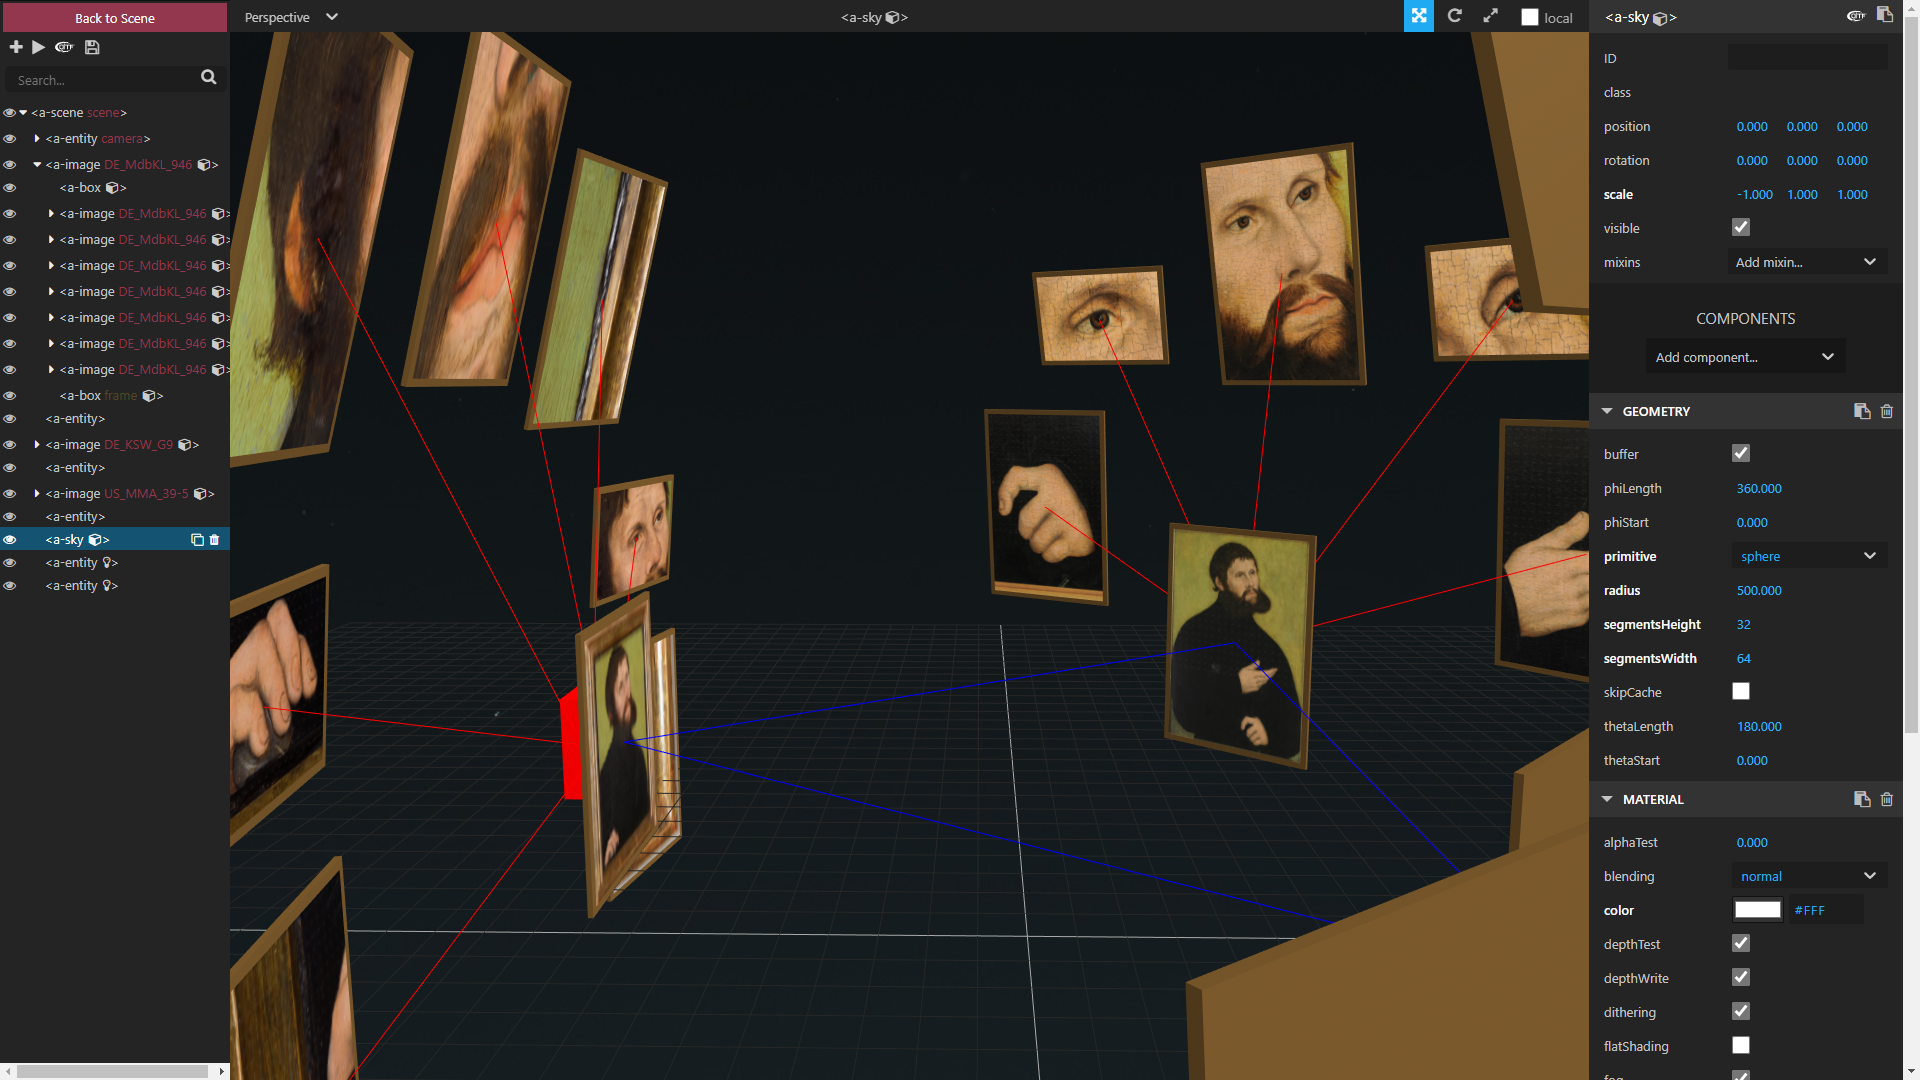
\includegraphics[scale=0.3]{img/coding/neural-network1.png}
          \caption[Übersicht des neuronalen Netzes aus der Inspektor-Perspektive von A-Frame.]{Übersicht des neuronalen Netzes aus der Inspektor-Perspektive von A-Frame. [Quelle: Eigene Darstellung].}
          \label{fig:neural-network1}
        \end{figure} \\ \\ \\
        Für die Fortbewegung zwischen den jeweiligen Verbindungen wird die
        zuvor beschriebene Standing Area wiederverwendet. Der Prototyp des
        neuronalen Netzes weist darüber hinaus eine horizontale wie auch 
        vertikale Fortbewegung auf, wodurch die Darstellung der 
        Standing Area verändert wurde. 
        So basiert die Komponente statt auf einem
        \texttt{<a-box>}-Tag auf einem \texttt{<a-sphere>}-Tag 
        (siehe Abb. \ref{fig:neural-network2}). Diese veränderte
        Darstellung führt zu einer fehlerhaften Anzeige des zuvor genutzten
        Icons, sodass die Komponente \texttt{standing-area} angepasst wurde.
        Diese nimmt über das Schema die Eigenschaft \texttt{icon} entgegen.
        Durch einen \texttt{boolean}-Wert kann das Icon aus- bzw. eingeblendet
        werden (siehe Abb. \ref{fig:neural-network2}).
        \begin{figure}
          \centering
          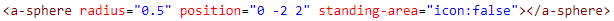
\includegraphics{img/coding/neural-network2.png}
          \caption[Standing Area Komponente auf Basis einer \texttt{<a-sphere>}.]{Standing Area Komponente auf Basis einer \texttt{<a-sphere>}. [Quelle: Eigene Darstellung].}
          \label{fig:neural-network2}
        \end{figure}
  \section{Ergebnisse}
    A-Frame als Framework hat gezeigt, dass sich das Entwickeln von Prototypen
    für das Web in einem fortgeschrittenen Stadium befindet. Das Framework
    bietet Möglichkeiten alle notwendigen Sinne anzusprechen, um eine
    immersive VR-Erfahrung zu bieten. 
    Der Einsatz von HTML für das Prototyping und die zusätzliche 
    Option zur Einbindung von JavaScript, gibt dem Framework alle
    notwendigen Funktionen zur Entwicklung einer entweder einfachen
    oder umfangreichen Anwendung. \\
    Der \textbf{Technische Prototyp} ermöglichte den Einstieg in 
    die Entwicklung mit A-Frame und bot darüber hinaus eine gute 
    Übersicht über die Möglichkeiten zur Darstellung von Gemälden 
    und Nahaufnahmen Cranachs. 
    Durch die einfache Schnittstelle über HTML ließen sich sehr
    schnell erste Prototypen entwickeln und mit Hilfe von JavaScript 
    in ihrer Funktion erweitern. 
    A-Frame bietet die notwendigen Funktionen zur Darstellung von
    Bildern sowie zusätzlich die implementierte blickgesteuerte
    Ausführung gewisser Interaktionen. Diese bereits bestehenden
    Grundlagen ermöglichten das Einsparen gewisser Entwicklungszeit.    
    Durch das Komponentensystem, 
    welches A-Frame bietet, konnte redundanter Code
    vermieden werden. In diesem Prototypen wurden die wichtigsten
    Komponenten und ihre Funktionen implementiert, welches die
    Entwicklung der weiteren Prototypen vereinfachte.
    Der zweite Prototyp, die \textbf{Werkstatt Lucas Cranachs}, 
    umfasst unterschiedliche Informationen eines Tages aus dem Jahr 1521.
    Die Dokumente auf dem Tisch ermöglichen dazu weitere Eindrücke
    über vergangene Geschehnisse Cranachs.
    Die Kombination von visueller und akustischer Darstellung schafft
    dabei eine immersive VR-Erfahrung. Zudem wird durch die
    Umgebung, die einer Werkstatt ähnelt, das Gefühl der Präsenz verstärkt.
    Der letzte Prototyp \textbf{Neuronales Netz} verstärkt das Datenverständnis
    des jeweiligen Benutzers, da auf einen Blick alle vorhandenen Daten und
    deren Beziehungen zueinander erkennbar sind. \\
    Der Benutzer sieht alle
    Gemälde über Junker Jörg, die aktuell im Cranach Digital Archive verfügbar
    sind und kann diese in direktem Vergleich betrachten.
  \section{Diskussion}
    Die Prototypen haben erfolgreich gezeigt, dass virtuelle Welten innerhalb
    eines Browsers ohne ein großes Team entwickelt werden konnten. Auch das
    Ausführen der Prototypen in der VR-Brille oder auf einem mobilen Endgerät 
    haben funktioniert. Je nach Anzahl der Gemälde oder Dokumente wird
    eine schnelle Internetverbindung und ausreichend Datenvolumen benötigt,
    da die zu herunterladenden Inhalte umfangreich sein können. Das
    Navigieren ohne 3D-Eingabegeräte ist funktional und stellt keine Hürde
    bei der Verwendung dar.
    Sofern die Webanwendung auf einem Server hochgeladen und über eine IP
    oder Domain erreichbar ist, kann jedes Endgerät 
    auf diese virtuelle Welt zugreifen.
    Auch die Leistung, welche benötigt wird, kann von einer eigenständigen
    VR-Brille oder einem modernen Smartphone erbracht werden. \\
    Obwohl es sich bei der Implementation um eine Webtechnologie handelt
    und diese in der Theorie von jedem modernen Browser aufgerufen werden
    kann, konnte nicht mit jedem Browser eine erfolgreiche VR-Erfahrung
    erreicht werden. Für das Smartphone war es möglich, 
    die Anwendung über die Browser
    Microsoft Edge, Google Chrome, Samsung
    Internet und Firefox ohne einen VR-Modus zu betrachten. 
    Ein Klick auf den VR-Button schaltete erfolgreich
    auf die VR-Ansicht um. 
    Die Browser Brave und Opera konnten jedoch lediglich 
    die normale 3D-Ansicht der Anwendung auf dem Smartphone darstellen
    und ermöglichten eine Rotation nur innerhalb der Y-Achse per Touch.
    Dies lässt sich auf die fehlende Unterstützung von WebXR zurückführen\footnote{Can I use | \url{https://caniuse.com/?search=webxr} (22.11.2020).}. \\
    Innerhalb der VR-Brille konnte die Webanwendung erfolgreich mit dem
    Oculus Browser und Firefox Reality getestet werden. Auch die Navigation
    innerhalb der VR-Anwendung erfolgte problemlos. \\
    Beim ersten Laden der
    Anwendung konnte jedoch ein kurzes Standbild festgestellt werden. Dies 
    führte kurzzeitig zum Bruch der \textbf{Ortsillusion}. Nachdem 
    die Anwendung alle Dateien erfolgreich geladen hatte, wurde der Bruch
    wieder aufgehoben.
    Des weiteren verläuft der Wechsel zwischen einem Gemälde Gemälde 
    und einer Nahaufnahme mit einer geringen Verzögerung.
    Die Bildhöhe passt sich an die der Detailaufnahme an,
    wird allerdings nicht simultan eingeblendet.
    Beide Probleme lassen sich auf die umfangreichen Dateigrößen und 
    die damit verbundenen Ladezeiten zurückführen.
    Dieses Problem lässt sich durch die Installation der Anwendung
    als PWA beheben, da die Bilddateien auf das Gerät geladen
    werden. \\ \\ \\
    Der Prototyp \textbf{Lucas Cranachs Werkstatt} kann durch das Erstellen
    von professionellen und hochauflösenden 3D-Modellen und Texturen
    einen höheren Realismus erhalten, was zu einer immersiveren
    VR-Erfahrung beitragen kann. Durch das Gestalten mehrerer Räume,
    könnten verschiedene
    Gemälde gezeigt werden, die in diesem Jahr entstanden sind oder an
    welchen Cranach aktuell gearbeitet hat. 
    Maschinen für die Druckgrafik könnten nachgestellt werden.
    Die Darstellung von Cranach in seiner Werkstatt, wie er an
    einem neuen Gemälde arbeitet, würde die Authentizität der VR-Erfahrung
    ebenfalls fördern. Diese Implementierung müsste jedoch gut umgesetzt sein,
    da ansonsten ein Bruch der \textbf{Plausibilitätillusion}
    entstehen könnte. \\
    Da das Cranach Digital Archive über eine große Datenbank verfügt,
    könnte im Stil des Prototyps \textbf{Neuronales Netz} ein 
    umfangreiches Netz aufgebaut werden, welches
    automatisiert generiert wird. Dabei könnten verschiedene 
    Filtermöglichkeiten für die einzelnen Verbindungen zwischen den 
    Gemälden implementiert werden. So könnten komplexe Beziehungen
    zwischen Gemälden und auch Dokumenten visuell dargestellt werden.
    Durch eine dreidimensionale, freie Bewegung in dem virtuellen Raum 
    wären dem Benutzer keine Grenzen in der Betrachtung der Daten gesetzt.
    Bei dieser Lösung muss jedoch eine schnelle Internetverbindung 
    gewährleistet sein oder die Möglichkeit bestehen, die Webanwendung
    als PWA zu installieren. \\
    Eine weitere Darstellungsmöglichkeit könnte ein Infrarot-Modus bieten,
    in welchem die verschiedenen Schichten eines Gemäldes herausgestellt
    werden können. \\ 
    Dieser Ansatz könnte neben der 
    grundlegenden Wissensvermittlung für 
    beispielsweise kunsthistorische Analysen hilfreich sein. \\
    Ähnlich zum Deutschen Auswandererhaus haben die entwickelten Prototypen 
    eine blickorientierte Steuerung und sind ohne 3D-Eingabegeräte funktionsfähig.
    Zusätzlich zum Storytelling-Ansatz konnte ein weiterer Prototyp entwickelt 
    werden, welcher die meisten Daten zu den Gemälden des
    Junker Jörg in einer Szene übersichtlich darstellt.
    Die Anwendungen des Deutschen Auswandererhauses,
    des Deutschen Museums in München und des Städel Museums sind 
    in ihrer Umsetzung professioneller und detailreicher, 
    wodurch eine immersivere und authentischere
    VR-Erfahrung geboten wird. Dennoch können die entwickelten 
    Prototypen, in Hinblick auf die verfügbaren Ressourcen 
    innerhalb dieses Projektes, ebenfalls eine
    immersive und interessante Darstellung und Interaktionsmöglichkeit mit
    Ausstellungsstücken des Cranach Digital Archives bieten.
    Darüber hinaus ermöglichen die vorliegenden Prototypen eine
    umfangreichere Erfahrung im Vergleich zur Museumsführung des
    Archäologischen Museums in Hamburg anhand von 360-Grad-Bildern. \\ 
    Demnach könnten die entwickelten Prototypen mit ein wenig 
    Feinschliff auf dem Markt vorhandener Anwendungen mithalten.
  \section{Fazit}
    Für die Gestaltung einer immersiven und qualitativ bzw. 
    quantitativ hochwertigen VR-Erfahrung, müssen zunächst 
    die Wahrnehmungsaspekte des Menschen berücksichtigt werden.
    Je mehr Sinne angesprochen werden,
    desto immersiver die Erfahrung für den Benutzer. 
    Die in Kapitel \ref{Wahrnehmungsaspekte} genannten Aspekte der Wahrnehmung
    konnten teilweise vollständig implementiert werden und verbesserten
    die Immersion der VR-Erfahrung. \\
    Die \textbf{Ortsillusion} konnte in allen drei Prototypen erreicht 
    werden. 
    Im Vergleich eignen sich VR-Brillen dafür besser als Smartphones,
    da diese eine höhere eine höhere
    Bildschirmauflösung und besseres Tracking bieten.
    Nichtsdestotrotz sind Smartphones für VR-Anwendungen 
    eine gute Alternative. \\
    Die \textbf{Plausibilitätsillusion} wurde in keiner der 
    Prototypen gebrochen, da wenig Platz für Fehler 
    vorhanden ist. Das Entwickeln von virtuellen Welten sollte
    deshalb immer agil stattfinden und jede neue Funktion erprobt 
    werden. So können auftretende Fehler sofort behoben
    und Funktionen, die eventuell zu komplex oder nicht authentisch
    sind, sofort überarbeitet werden. Je nach Größe des Problems
    kann diese Funktion vollständig weggelassen werden. \\
    Die Möglichkeit des Wechsels zwischen Nahaufnahme und Gemälde
    sowie die Vertonung von Cranachs Dokumenten kann
    das Interesse und die Aufmerksamkeit 
    innerhalb der Anwendungen steigern.
    Diese Details sind einfach umzusetzen
    und können dennoch eine große Wirkung auf den Anwender haben. \\
    Die Aufgabe, Informationen und Emotionen zu verbreiten, kann durch
    Virtual Reality an eine große Zielgruppe herangetragen werden. 
    Durch den Einsatz von Webtechnologien für die 
    Umsetzung von VR-Anwendungen wird niemand anhand 
    der Technologiewahl ausgeschlossen.
    Besonders mit einem modernen Smartphone 
    oder einer VR-Brille kann jeder Mensch
    diese Anwendung aufrufen. Es ist keine Installation notwendig
    und die VR-Erfahrung kann sofort aufgerufen werden. \\
    Ein Museum dürfte nicht weniger Besucher durch eine online abrufbare
    Anwendung bekommen, da originale Ausstellungsstücke einen nicht
    reproduzierbaren Charakter besitzen. Die virtuellen Darstellungen
    haben nicht die gleiche Authentizität wie ihre originalen Gegenstücke.
    Solch eine Webanwendung kann als Marketingwerkzeug betrachtet
    werden, da viele Besucher, die vorher eine Onlineausstellung
    betrachtet haben, dazu neigen können, dass Museum auch in der realen
    Welt zu besuchen. Daraus würde sich eine Chance für Museen abzeichnen, 
    eine größere Zielgruppe anzusprechen. \\
    Heutige moderne Browser können umfangreiche VR-Erfahrungen ausführen.
    Dank Schnittstellen,
    wie WebGL und WebXR sowie Frameworks wie beispielsweise A-Frame, 
    können Webanwendungen teilweise mit nativer Software mithalten. 
    Sofern die Ressourcen
    vorhanden sind, können professionelle und realistische virtuelle
    Welten gestaltet werden.  \\ \\
    Dabei können die Schnittstellen auf
    die meisten VR-Geräte zugreifen und ihre 3D Eingabegeräte erkennen. \\
    Zusammenfassend wurde das einleitend angesprochene Ziel 
    unterschiedlicher
    Darstellungs- und Interaktionsmöglichkeiten von Cranachs 
    Gemälden und Dokumenten in virtuellen Welten erreicht.
    Dabei zeigen die erarbeiteten Ansätze
    lediglich vereinzelte Möglichkeiten, die neben zahlreichen
    Weiteren bestehen. \\
    A-Frame als Framework zur Entwicklung von VR-Anwendungen 
    lässt sich schnell erlernen und unterstützt bei der 
    Entwicklung durch seine Einfachheit. \\
    Durch das Prototyping mit HTML und das mögliche Erweitern durch 
    JavaScript konnte A-Frame vielfältig eingesetzt werden.
    Die Möglichkeit vollständig auf Three.js zuzugreifen 
    erlaubt umfangreiche Darstellungen in Virtual Reality.
    Der Einsatz von realistischen Shadern, Physik und 
    hochauflösenden Umgebungen könnte
    die Immersion um ein vielfaches steigern. \\
    Das Potenzial der Entwicklung von VR-Webanwendungen für Museen
    ist enorm, da ein innovativer, zugänglicher und interessanter 
    Ansatz für  einen Wissensaustausch stattfinden kann. 
    Dabei ist die Zielgruppe, die erreicht werden kann,
    größer als die der klassischen Museumsbesucher.
    Durch moderne Technologien, wie zum Beispiel A-Frame,
    können bereits aktuell Anwendungn entwickelt werden, die alle
    Standards und Aspekte bedienen, welche für eine qualitativ
    wie auch quantitativ hochwertige VR-Erfahrung notwendig sind.
  \section{Nachwort}
    Nachdrücklich bedanke ich mich für die angenehme Zusammenarbeit
    mit Prof. Christian Noss, Matthias Groß und Uwe Müsse. Darüber
    hinaus gilt mein Dank ebenfalls dem Team des Cranach Digital 
    Archives für die bedinungslose Bereitstellung der digitalen 
    Daten sowie für die Beantwortung jeglicher Fragen. \\
    Im Rahmen dieser Bachelorarbeit wurde das im Studium erlangte
    Wissen gefestigt, das wissenschaftliche Arbeiten 
    vertieft und trotz auftretender Probleme umfangreiche 
    Erfahrungen im zielorientierten
    Entwickeln gewonnen. Zudem wurde durch die Kombination
    unterschiedlicher Wissenschaften die Wichtigkeit 
    interdisziplinärer Forschung erkannt. \\    
    Abschließend spreche ich mich positiv für das
    Thema dieser Bachelorarbeit aus, welches
    unter anderen repräsentativ für den 
    Bereich der Medieninformatik ist. \newpage
  \section{Quellenverzeichnis}
    \printbibliography
  \newpage
  \pagestyle{empty}
  \section*{Erklärung über die selbständige Abfassung der Arbeit}
    \addcontentsline{toc}{section}{Erklärung über die selbständige Abfassung der Arbeit}
    Ich versichere, die von mir vorgelegte Arbeit selbständig verfasst zu haben.
    Alle Stellen, die wörtlich oder sinngemäß aus veröffentlichten oder nicht veröffentlichten Arbeiten anderer entnommen sind,
    habe ich als entnommen kenntlich gemacht.\\ 
    Sämtliche Quellen und Hilfsmittel, die ich für die Arbeit benutzt habe, sind
    angegeben. Die Arbeit hat mit gleichem Inhalt bzw. in wesentlichen Teilen noch keiner anderen Prüfungsbehörde vorgelegen.\\\\
    \begin{tabular}{cp{7cm}}
      & \\ 
      & \\ \hline
      \small (Ort, Datum, Unterschrift) & \normalsize \\
    \end{tabular}
  \newpage
  % Unbeschriftetes Abschlussblatt (Leere Seite)
  \thispagestyle{empty}
  \section*{}  
          
\end{document}